%% 03-the-ai-native-agent-framework.tex -- generated by tools/build_from_docx.py; edit freely

\hypertarget{the-ai-native-agent-framework}{%
\section{The AI-Native Agent Framework}\label{the-ai-native-agent-framework}}

The agentic framework specifies how a management function contributed by
any partner --- an algorithm, a trained model, an application ---
becomes an autonomous agent that observes, reasons, decides and acts on
the network within bounds that are set, held and enforced by the
platform rather than by the contributed function itself. Its structural
unit is the tuple of four capabilities inherited from MonB5G: the
Monitoring System (MS), the Analytics Engine (AE), the Decision Engine
(DE) and the Actuator (ACT). The framework extends the tuple into an
agent: a tuple instantiated against a declared objective, carrying
declared scope, declared behavior and granted authority, placed in one
or more of the architecture's domains and governed through its life by
the IDMO and the DMOs.

The framework is technique-neutral. The logic inside a capability may be
a trained model, a reinforcement-learning policy, a reasoner based on a
language model, an optimization solver, a digital twin or a set of
rules. The framework does not constrain how a capability reasons. It
constrains what the capability may consume and produce, what it may
change and when, and what the platform establishes before, during and
after it acts. One proposition underlies every rule that follows:
authority over live infrastructure is granted to an agent in proportion
to what the platform can verify about it, and is exercised only within
bounds that the platform holds.

\hypertarget{terms-notation-and-conventions}{%
\subsection{Terms, Notation and Conventions}\label{terms-notation-and-conventions}}

\hypertarget{normative-language}{%
\subsubsection{Normative language}\label{normative-language}}

The keyword \emph{shall} denotes a mandatory requirement and \emph{shall
not} a prohibition. \emph{Should} denotes a recommendation; a deviation
from it has no consequence beyond any stated with the recommendation.
\emph{May} denotes a permission. A requirement applies to the party
named in it; where no party is named, it applies to the platform.
Sentences in the indicative mood describe behavior that follows from
requirements stated elsewhere and introduce no further obligation.
Tables that define terms, fields, values, rules or checks are normative;
figures are informative.

The platform is the combination of the tuple registry, admission, the
capability runtimes and the gates they operate, realized within the IDMO
and the DMOs. Where a requirement falls on the IDMO or on a DMO
specifically, that party is named.

\hypertarget{terms-and-definitions}{%
\subsubsection{Terms and definitions}\label{terms-and-definitions}}

The terms of Table 3-1 carry the meaning given there throughout the
chapters of this specification. Three terms that are easily confused are
kept distinct: a \emph{message envelope} is the metadata carried by
every message; an \emph{action envelope} is a region of an agent's
action space pre-authorized by the conflict fabric; an \emph{authority
envelope} is the scope and the limits within which a DMO acts on a
delegation without referring to the IDMO.

\begin{wptable}{3-1}

\begin{longtable}[]{@{}
  >{\raggedright\arraybackslash}p{(\columnwidth - 2\tabcolsep) * \real{0.2250}}
  >{\raggedright\arraybackslash}p{(\columnwidth - 2\tabcolsep) * \real{0.7750}}@{}}
\caption{Terms and definitions}\tabularnewline
\toprule\noalign{}
\begin{minipage}[b]{\linewidth}\raggedright
\textbf{Term}
\end{minipage} & \begin{minipage}[b]{\linewidth}\raggedright
\textbf{Definition}
\end{minipage} \\
\midrule\noalign{}
\endfirsthead
\toprule\noalign{}
\begin{minipage}[b]{\linewidth}\raggedright
\textbf{Term}
\end{minipage} & \begin{minipage}[b]{\linewidth}\raggedright
\textbf{Definition}
\end{minipage} \\
\midrule\noalign{}
\endhead
\bottomrule\noalign{}
\endlastfoot
\textbf{Action} & A change of one or more control parameters of a
managed object, requested as an instance of an action type of the
agent\textquotesingle s action space. \\
\textbf{Action envelope} & A bounded region of an
agent\textquotesingle s action space, with a validity window and a rate
limit, pre-authorized by the conflict fabric; actions inside it proceed
without per-action mediation. \\
\textbf{Action space} & The action types an agent may request, each with
parameter bounds, rate limit, stability controls, verification method,
idempotency, rollback and mediation path (Section 3.5.8). \\
\textbf{Admission} & The procedure by which the platform checks a
descriptor, and the values bound to it at instantiation, against the
registry, the catalog and the proposed placement, and either rejects the
agent or registers it with an authority ceiling and an effective latency
class. \\
\textbf{Agent} & A tuple instantiated against one or more objectives,
with scope, declared behavior, granted authority and identity. \\
\textbf{Agent descriptor} & The machine-readable, versioned and signed
document that declares an agent type (Section 3.5). \\
\textbf{Agent instance} & One realization of an agent descriptor in one
domain or, for a global agent, at the IDMO; identified by
agentInstanceId or globalAgentId and by a generation. \\
\textbf{Assurance} & The account of an agent\textquotesingle s operation
returned to the requester, the party that issued its descriptor for
instantiation, and assembled by the platform: objective status;
actuation outcomes, including unverified and unresolved counts;
authority changes; unachievable-objective events; conflict
statistics. \\
\textbf{Authority ceiling} & The highest authority state an agent
instance may hold (Section 3.4.7). \\
\textbf{Authority envelope} & The scope and quantitative limits, with a
validity window, within which a DMO acts on a delegation without
referral to the IDMO. \\
\textbf{Authority state} & The registry-held state that determines what
an agent instance may do at a given moment (Table 3-12). \\
\textbf{Binding} & The realized connection that carries one logical flow
between two endpoints for one generation; of class
LOCAL\_\allowbreak{}RUNTIME, DATA\_\allowbreak{}CONTINUUM, SMB or
SOUTHBOUND. \\
\textbf{Capability} & One of the four functions of the tuple: Monitoring
System (MS), Analytics Engine (AE), Decision Engine (DE), Actuator
(ACT). \\
\textbf{Capability mode} & The declaration of who performs a capability
for an agent: full, partial, delegated or none (Table 3-8). \\
\textbf{Capability runtime} & The platform component that hosts the
contributed logic of one capability, performs all its binding exchanges,
computes its platform-computed fields and operates its gates. \\
\textbf{Composition class} & The class derived from the four capability
modes: closed\_\allowbreak{}loop, open\_\allowbreak{}loop, analytics,
observation or actuation\_\allowbreak{}service (Table 3-9). \\
\textbf{Conflict fabric} & The mediation service, contributed by WP4,
that returns verdicts on submitted intents, grants action envelopes and
distributes conflict-freedom policies. \\
\textbf{Contributed logic} & The partner-supplied code that performs the
function of one capability. \\
\textbf{Control parameter (CP)} & A configurable property of a managed
object that an action changes; defined in the catalog. \\
\textbf{Control scope} & The managed objects and control parameters that
an agent may change. \\
\textbf{Delegation} & A DomainAgentDelegation: the document by which a
global agent assigns an outcome-oriented responsibility to one domain
(Section 3.5.21). \\
\textbf{Effective latency class} & The latency class assigned at
admission from the computed effective loop latency (Section 3.8.3). \\
\textbf{Generation} & A non-negative integer, assigned by the owning DMO
or IDMO, identifying one deployment of an agent instance; incremented on
every placement, restart, migration, model update and binding change,
and on migration or termination of the underlying domain service. \\
\textbf{Insight} & The semantic object produced by the AE. \\
\textbf{Intent} & The semantic object produced by the DE: a requested
action with targets, parameters, validity window and rationale. \\
\textbf{Loop budget} & The declared upper bound on an
agent\textquotesingle s loop time. \\
\textbf{Loop time} & The time from the event time of the earliest
observation contributing to a decision to the enforcement of the
resulting action (Section 3.8.2). \\
\textbf{Managed object} & An entity whose state an agent observes or
changes: node, link, path, slice, flow, service, user equipment or
device; for a global agent, a delegation. \\
\textbf{Mediation} & The submission of an intent to the conflict fabric
and the receipt of its verdict. \\
\textbf{Message envelope} & The metadata that every message carries on
every binding (Table 3-6). \\
\textbf{Observation} & The semantic object produced by the MS. \\
\textbf{Outcome} & The semantic object produced by the ACT, stating one
of the four results of an actuation. \\
\textbf{Platform} & The tuple registry, admission, the capability
runtimes and the gates they operate, realized within the IDMO and the
DMOs. \\
\textbf{Registry} & The store of every agent instance\textquotesingle s
identity, authority and bounds, held by each DMO for its local agents
and by the IDMO for global agents; the single source of authority
truth. \\
\textbf{Scope tags} & Machine-comparable labels --- region, site, slice,
tenant, technology --- attached to every message for routing and
conflict detection. \\
\textbf{Service request (RFS)} & The resource-facing service request
that the IDMO produces for one domain by decomposing a customer-facing
service; carries no agent content. \\
\textbf{Tuple} & The four capabilities MS, AE, DE and ACT, each with a
declared mode, composed in that order into a closed management loop. \\
\textbf{Type catalog} & The versioned registry of metrics, control
parameters, action and insight types, objective KPIs, verification
methods, controller bindings, source kinds, reason codes and service
contracts (Section 3.6). \\
\textbf{Verdict} & The response of the conflict fabric to a submitted
intent: allow, modify, defer or deny, with a reason code and the
identity of the resolving authority. \\
\end{longtable}

\end{wptable}

\hypertarget{identifiers}{%
\subsubsection{Identifiers}\label{identifiers}}

The identifiers of Table 3-2 are used by every party to the framework.
Identifier names follow the information model of the service request and
are written in camel case; descriptor field names follow the descriptor
scheme and are written in snake case.

\begin{wptable}{3-2}

\begin{longtable}[]{@{}
  >{\raggedright\arraybackslash}p{(\columnwidth - 6\tabcolsep) * \real{0.2063}}
  >{\raggedright\arraybackslash}p{(\columnwidth - 6\tabcolsep) * \real{0.2187}}
  >{\raggedright\arraybackslash}p{(\columnwidth - 6\tabcolsep) * \real{0.1625}}
  >{\raggedright\arraybackslash}p{(\columnwidth - 6\tabcolsep) * \real{0.4125}}@{}}
\caption{Identifiers}\tabularnewline
\toprule\noalign{}
\begin{minipage}[b]{\linewidth}\raggedright
\textbf{Identifier}
\end{minipage} & \begin{minipage}[b]{\linewidth}\raggedright
\textbf{Assigned by}
\end{minipage} & \begin{minipage}[b]{\linewidth}\raggedright
\textbf{Unique within}
\end{minipage} & \begin{minipage}[b]{\linewidth}\raggedright
\textbf{Lifetime and use}
\end{minipage} \\
\midrule\noalign{}
\endfirsthead
\toprule\noalign{}
\begin{minipage}[b]{\linewidth}\raggedright
\textbf{Identifier}
\end{minipage} & \begin{minipage}[b]{\linewidth}\raggedright
\textbf{Assigned by}
\end{minipage} & \begin{minipage}[b]{\linewidth}\raggedright
\textbf{Unique within}
\end{minipage} & \begin{minipage}[b]{\linewidth}\raggedright
\textbf{Lifetime and use}
\end{minipage} \\
\midrule\noalign{}
\endhead
\bottomrule\noalign{}
\endlastfoot
\textbf{descriptor\_\allowbreak{}id} & Contributor, at catalog
registration & Global & Permanent. URN of the form
urn:unity6g:agent:\textless publisher\textgreater:\textless name\textgreater;
stable across versions. \\
\textbf{version} & Contributor & descriptor\_\allowbreak{}id &
Permanent. Semantic Versioning 2.0.0; immutable once admitted. \\
\textbf{intentId} & Intent layer & Global & Lifetime of the intent;
correlates the service orchestration pipeline and takes no part in agent
isolation. \\
\textbf{rfsId} & IDMO & Global & Lifetime of the domain service
request. \\
\textbf{assignedDomainId} & IDMO, at domain registration & Global &
Lifetime of the domain\textquotesingle s registration. \\
\textbf{domainServiceId} & DMO & Domain & Lifetime of the domain service
realizing the RFS. \\
\textbf{agentInstanceId} & Requesting party: the IDMO for a global
agent; the DMO for a local agent or when realizing a delegation & Global
(UUID) & Lifetime of the agent instance; confirmed by the DMO in the
resolved configuration. \\
\textbf{globalAgentId} & IDMO & Global (UUID) & Lifetime of a global
agent; carried in the provenance of every message of the local agents
that realize its delegations. \\
\textbf{delegationId} & IDMO & Global (UUID) & Lifetime of a
delegation. \\
\textbf{generation} & DMO for local agents; IDMO for global agents &
agentInstanceId & Monotonic, never reused; carried in every message. \\
\textbf{correlationId} & DE runtime, when an intent is emitted & Global
(UUID) & Until the final outcome of the intent is reported. \\
\textbf{bindingId} & DMO & agentInstanceId & One generation. \\
\textbf{service\_\allowbreak{}id} & IDMO & SMB & Lifetime of the
service; names the per-service SMB topic. \\
\textbf{grantId} & Conflict fabric & Domain & Validity window of an
action envelope or distributed policy grant. \\
\textbf{messageId} & Producing runtime & Global (UUID) & Lifetime of the
message; used for de-duplication and provenance. \\
\end{longtable}

\end{wptable}

The identifiers descriptor\_\allowbreak{}id, assignedDomainId and
agentInstanceId together form the unit of isolation. Two agent instances
that differ in this triple share no policy state, model state, decision
history, action correlation, evaluation window or lifecycle, even where
they execute on the same infrastructure. The local agent identifier of
the hierarchical instantiation model and the agentInstanceId denote the
same object; this specification uses agentInstanceId for both.

\hypertarget{value-types-formats-and-schema-languages}{%
\subsubsection{Value types, formats and schema languages}\label{value-types-formats-and-schema-languages}}

Descriptors, delegations and message payloads use the value types of
Table 3-3. Descriptors are written in YAML 1.2 or in JSON, which are
equivalent; the normative rendering of the descriptor as a JSON Schema
is given in Annex A. That rendering is the definition of the
descriptor's structure: where a field table of Section 3.5 and the
schema of Annex A differ in detail, the schema governs, and the field
tables of this chapter are read as its description and its rationale.
The schema carries its own identifier and version and is revised on that
version alone, without revision of this chapter, provided the revision
introduces no obligation absent from the requirements of Section 3.11. A
descriptor is hashed for integrity after canonicalization under RFC
8785, so that a descriptor yields one digest independently of how it was
serialized. Message payloads are defined by semantic schemas written in
JSON Schema 2020-12 and held in the schema registry under an identifier
and a version. The serialization of a message is a property of its
binding and does not change its schema: messages on the service-based
management bus (SMB) are serialized as JSON; messages on a local runtime
binding use any encoding that preserves the schema; data products of the
Data Continuum map onto the NGSI-LD entity type that the data product
declares.

\begin{wptable}{3-3}

\begin{longtable}[]{@{}
  >{\raggedright\arraybackslash}p{(\columnwidth - 2\tabcolsep) * \real{0.1875}}
  >{\raggedright\arraybackslash}p{(\columnwidth - 2\tabcolsep) * \real{0.8125}}@{}}
\caption{Value types and formats}\tabularnewline
\toprule\noalign{}
\begin{minipage}[b]{\linewidth}\raggedright
\textbf{Type}
\end{minipage} & \begin{minipage}[b]{\linewidth}\raggedright
\textbf{Format}
\end{minipage} \\
\midrule\noalign{}
\endfirsthead
\toprule\noalign{}
\begin{minipage}[b]{\linewidth}\raggedright
\textbf{Type}
\end{minipage} & \begin{minipage}[b]{\linewidth}\raggedright
\textbf{Format}
\end{minipage} \\
\midrule\noalign{}
\endhead
\bottomrule\noalign{}
\endlastfoot
\textbf{id} & URN, or UUID version 4 (RFC 9562), as specified per
identifier. \\
\textbf{semver} & Semantic Versioning 2.0.0, for example 1.4.2. \\
\textbf{semver-range} & Space-separated comparator set, for example
\textgreater=1.2.0 \textless2.0.0. \\
\textbf{duration} & Decimal number followed by one of us, ms, s, min or
h, for example 7.5ms. \\
\textbf{timestamp} & RFC 3339, UTC, with microsecond precision. \\
\textbf{rate} & count/duration, for example 10/1s. \\
\textbf{ratio} & Decimal number in the interval {[}0, 1{]}. \\
\textbf{digest} & sha256: followed by 64 lower-case hexadecimal
digits. \\
\textbf{predicate} & Structured boolean condition: an object carrying
either a single comparison --- the operand, one of the comparators eq,
ne, lt, le, gt, ge, in, nin, exists or matches, and a literal value or a
second operand --- or one of the combinators allOf, anyOf or not over
nested predicates. Operands name fields declared in the same descriptor
only. Nesting depth does not exceed four. \\
\textbf{schema-ref} & identifier@version of a JSON Schema 2020-12
document in the schema registry. \\
\textbf{type-ref} & identifier@version of an entry of the type
catalog. \\
\textbf{enum} & Exactly one of the listed values; case-sensitive. \\
\textbf{list, map, object} & As in JSON. The order of a list is
significant only where stated. \\
\end{longtable}

\end{wptable}

\hypertarget{principles}{%
\subsection{Principles}\label{principles}}

Eleven principles govern the framework. Each is realized by requirements
of this chapter and of the chapters that follow; none is advisory.

\begin{itemize}
\tightlist
\item
  \textbf{Platform, not bespoke design.} Contributions are admitted onto
  the platform as tenants, against contracts. WP4 algorithms and WP5
  applications are the platform's first tenants, not its specification:
  a contribution the authors of this specification have never seen is
  admissible if it satisfies the contracts.
\item
  \textbf{Flexible declaration, strict admission.} A contribution is
  admitted at the authority its evidence supports --- full closed loop,
  reduced closed loop, advisory or monitoring only --- or it is
  rejected. No contribution is exempted from any check, and none is
  excluded from the platform because it cannot yet support full
  authority.
\item
  \textbf{Freedom in the algorithm, never in the guardrails.}
  Contributed logic is opaque to the platform and free in technique. The
  declarations through which the platform bounds it --- scope, action
  space, failure behavior, policies, interfaces and integrity --- are
  closed to extension.
\item
  \textbf{The platform computes what it can check.} Every quantity the
  platform can establish for itself --- the coverage of observation, the
  quality of the input to analytics, whether a model's input lies within
  its declared validity, the latency actually achieved, the outcome of
  an actuation --- is computed by the platform and never accepted from
  contributed logic. What the platform cannot verify is declared as
  unverifiable, admitted only within the limits of target and rate of
  Section 3.5.8, and counted in assurance.
\item
  \textbf{No self-approval.} A DE cannot authorize its own intents. An
  intent that affects a shared or contended resource reaches the ACT
  only after mediation by the conflict fabric, or within an action
  envelope or a distributed policy that the fabric has granted.
  Coordination is never inside the decision.
\item
  \textbf{No global runtime brain.} DEs are per domain and fast loops
  close locally. Intelligence at the IDMO sets objectives and bounds for
  domains through delegations on the non-real-time timescale; it does
  not issue control commands to infrastructure.
\item
  \textbf{End-to-end objectives are resolved once.} An end-to-end
  objective is held by a global agent and is resolved into per-domain
  portions once, when that agent is instantiated; a change is a new
  agent, not a re-resolution at runtime. Coherence between domains at
  runtime comes from that resolution, from the conflict fabric and from
  delegation updates on the non-real-time timescale.
\item
  \textbf{Technique neutrality.} The same contracts apply whichever
  technique realizes a capability. Whether a technique is admissible in
  a capability depends on what its output can be bounded to (Section
  3.4.6).
\item
  \textbf{Bounds first.} The latency classes and the bounds derived from
  the project KPIs are fixed before agents are defined, and agents are
  defined to fit them. An agent that cannot meet the bounds of a class
  does not hold that class: it is admitted at a class it can sustain, or
  it is rejected.
\item
  \textbf{Nothing fails silently.} Every actuation ends in one of four
  declared outcomes; a binding fault suspends the affected capability
  rather than letting it continue on a best-effort basis; and the
  requester receives objective status and actuation outcomes, including
  unverified and unresolved actuations, assembled by the platform.
\item
  \textbf{Coexistence.} Services managed conventionally, without agents,
  coexist with agent-managed services in the same deployment. The
  framework applies wherever an agent is requested, and it places
  conditions on conventionally managed functions only where they share
  control parameters with agents (Section 3.10).
\end{itemize}

\hypertarget{the-agent-as-a-tuple-of-capabilities}{%
\subsection{The Agent as a Tuple of Capabilities}\label{the-agent-as-a-tuple-of-capabilities}}

\hypertarget{the-four-capabilities}{%
\subsubsection{The four capabilities}\label{the-four-capabilities}}

An agent's closed loop is composed of four capabilities, inherited from
the MonB5G management tuple with their separation of concerns and their
order unchanged. Each capability has one kind of output, a boundary it
shall not cross, and a capability runtime supplied by the platform that
holds it to both (Figure 3-1, Table 3-4).

The Monitoring System produces evidence. Within its observation scope it
acquires measurements, counters, events, logs and state from
infrastructure and service components; normalizes units and time base;
aggregates over the declared window and computes the catalog-defined
metrics its descriptor declares, these being performed by the capability
runtime rather than by contributed logic so that a metric name denotes
one computation across the platform (Chapter 4); enriches each record
with the scope tags on which routing and conflict detection depend;
removes duplicates; and annotates quality. It does not score, forecast,
classify or propose causes, and it does not present as measured any
value it did not measure.

The Analytics Engine produces insight --- anomaly indications,
forecasts, classifications, derived KPIs and root-cause hypotheses ---
each accompanied by the model's own confidence. It holds no authority
and proposes no action; a root-cause hypothesis names a cause, not a
remedy. Because the AE holds no authority, its model can be replaced
without changing what the agent is permitted to do.

The Decision Engine produces intent: a requested change, expressed as an
action of the agent's registered action space, with targets, parameters,
a validity window and a structured rationale. It is the capability that
carries authority and is therefore the most constrained: it cannot
approve its own intents, and whenever its declared failure behavior is
absent or ambiguous at runtime it emits nothing.

The Actuator translates intent into commands of the authoritative
controller, submits them, verifies the result against the state of the
managed object through a path independent of the controller's
acknowledgement, and reports one of four outcomes. The ACT is a role and
not a privilege tier: conformant and extension agents actuate through
the same path, and containment resides in scope, bounds and mediation
rather than in a separate execution route.

\begin{figure}[htbp]
\centering
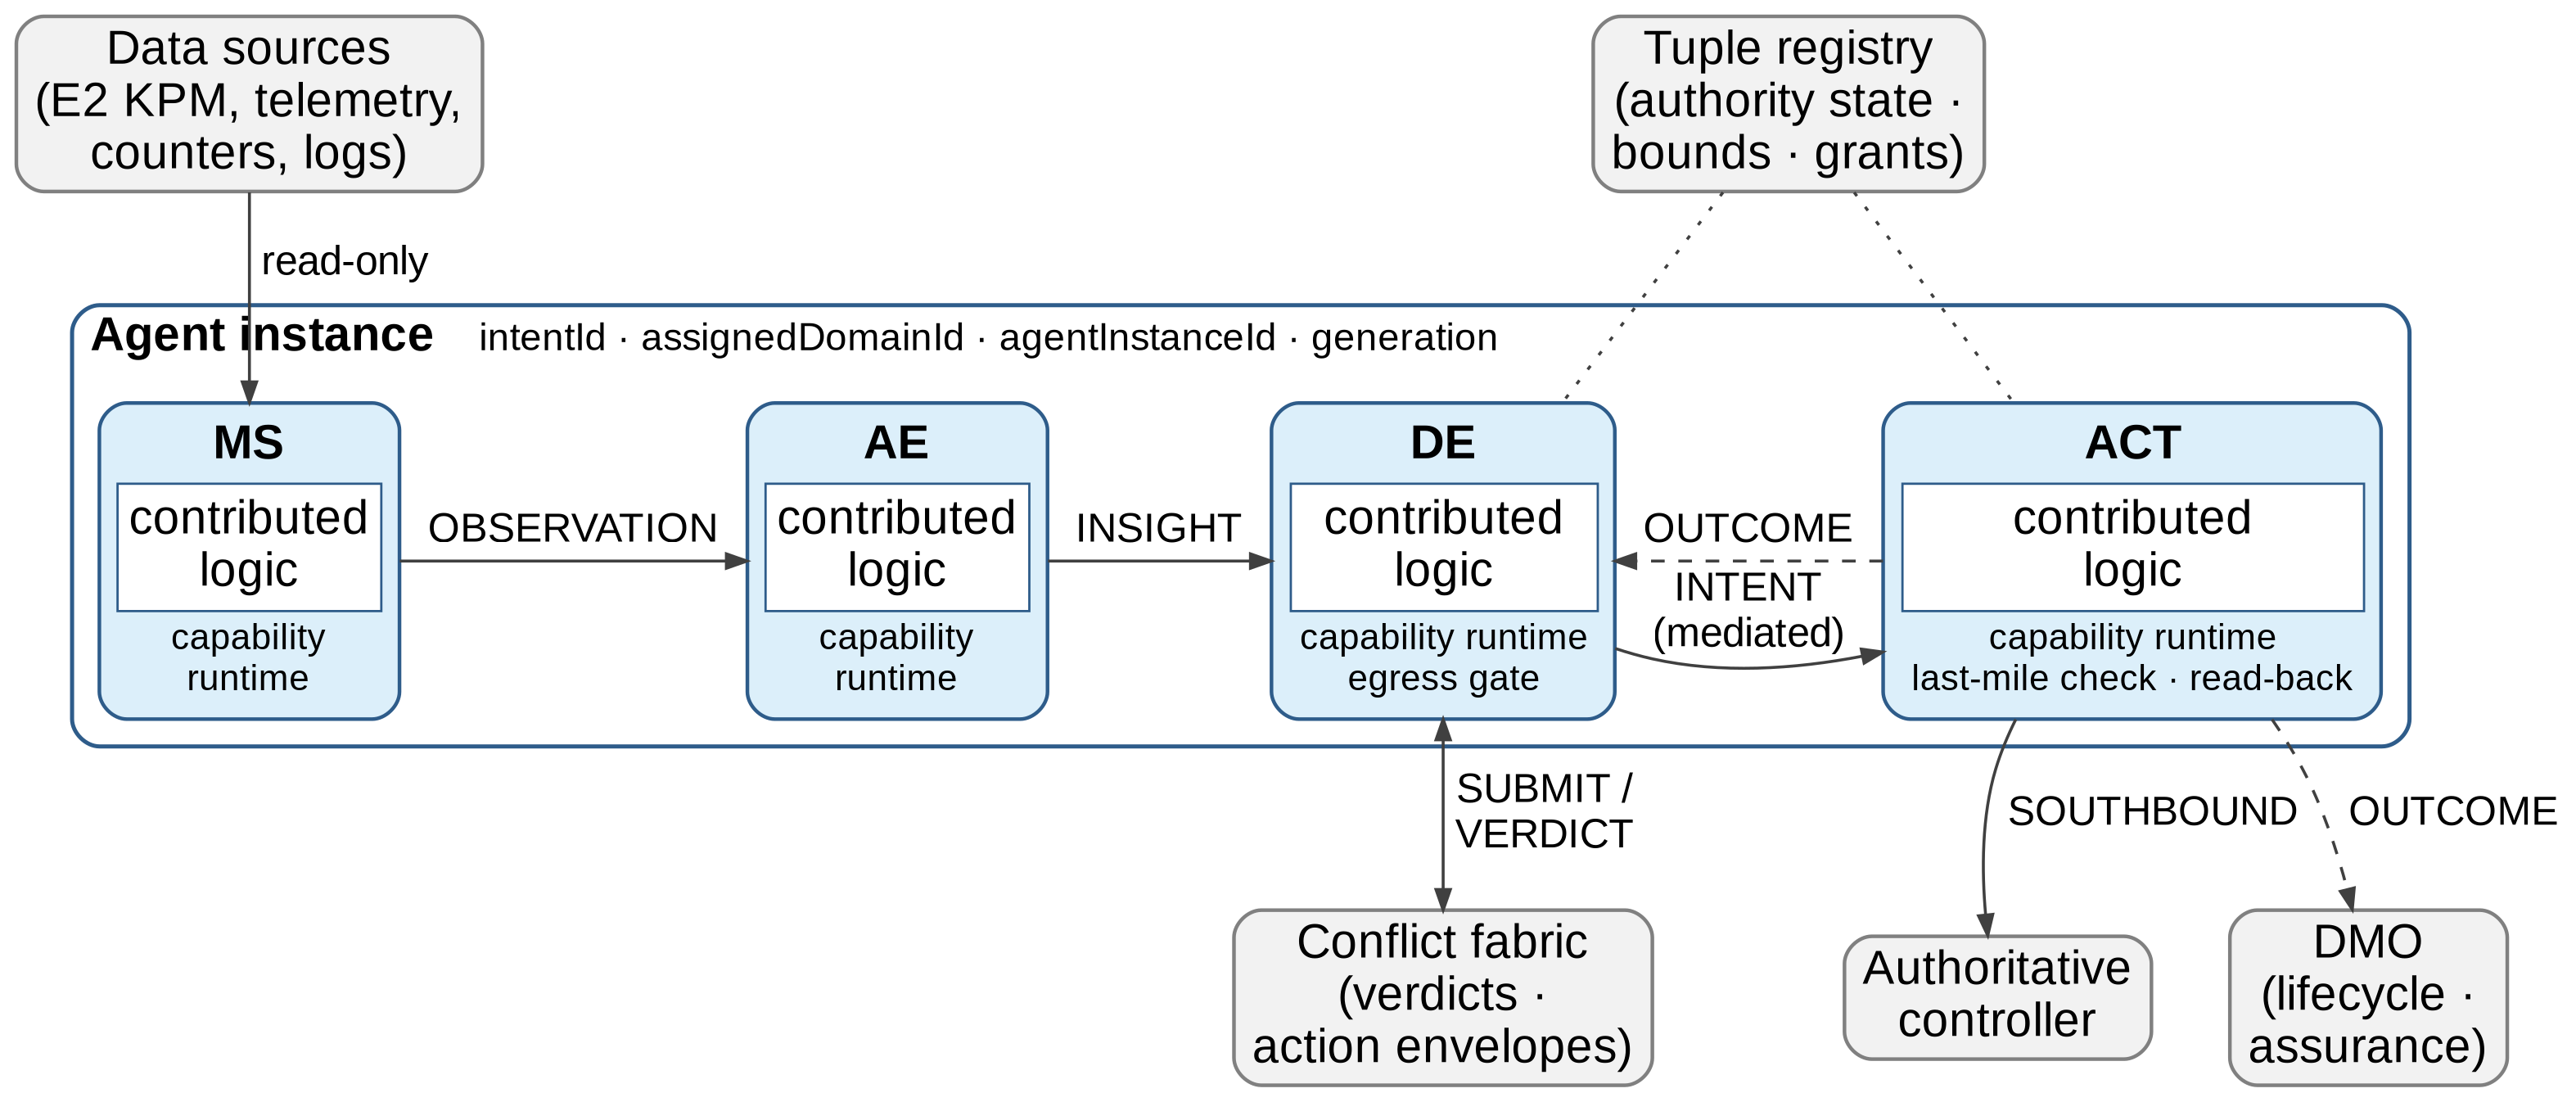
\includegraphics[width=\linewidth,height=0.45\textheight,keepaspectratio]{figures/image1.png}
\captionnum{3-1}
\caption{Anatomy of an agent instance}
\label{fig:3-1}
\end{figure}

\begin{wptable}{3-4}

\begin{longtable}[]{@{}
  >{\raggedright\arraybackslash}p{(\columnwidth - 8\tabcolsep) * \real{0.1312}}
  >{\raggedright\arraybackslash}p{(\columnwidth - 8\tabcolsep) * \real{0.2063}}
  >{\raggedright\arraybackslash}p{(\columnwidth - 8\tabcolsep) * \real{0.1937}}
  >{\raggedright\arraybackslash}p{(\columnwidth - 8\tabcolsep) * \real{0.2562}}
  >{\raggedright\arraybackslash}p{(\columnwidth - 8\tabcolsep) * \real{0.2126}}@{}}
\caption{The four capabilities}\tabularnewline
\toprule\noalign{}
\begin{minipage}[b]{\linewidth}\raggedright
\textbf{Capability}
\end{minipage} & \begin{minipage}[b]{\linewidth}\raggedright
\textbf{Consumes}
\end{minipage} & \begin{minipage}[b]{\linewidth}\raggedright
\textbf{Produces}
\end{minipage} & \begin{minipage}[b]{\linewidth}\raggedright
\textbf{Shall not produce}
\end{minipage} & \begin{minipage}[b]{\linewidth}\raggedright
\textbf{Typical placement}
\end{minipage} \\
\midrule\noalign{}
\endfirsthead
\toprule\noalign{}
\begin{minipage}[b]{\linewidth}\raggedright
\textbf{Capability}
\end{minipage} & \begin{minipage}[b]{\linewidth}\raggedright
\textbf{Consumes}
\end{minipage} & \begin{minipage}[b]{\linewidth}\raggedright
\textbf{Produces}
\end{minipage} & \begin{minipage}[b]{\linewidth}\raggedright
\textbf{Shall not produce}
\end{minipage} & \begin{minipage}[b]{\linewidth}\raggedright
\textbf{Typical placement}
\end{minipage} \\
\midrule\noalign{}
\endhead
\bottomrule\noalign{}
\endlastfoot
\textbf{MS} & Raw telemetry, events, logs and state from declared
sources, read-only & Observations, with coverage and data quality
signals & Scores, forecasts, classifications or confidence; any value
not measured & Device or edge, beside the data source \\
\textbf{AE} & Observations, or data products of the Data Continuum &
Insights, with model confidence, input quality and validity state &
Action identifiers, target configurations, parameter values to apply,
controller references & Edge, regional or central; principal consumer of
accelerators \\
\textbf{DE} & Insights (observations where the AE is none), objectives,
state, verdicts, outcomes & Intents, with structured rationale &
Controller-native commands; any intent that bypasses mediation & As the
loop\textquotesingle s latency class requires: DU/CU, Near-RT RIC,
regional or central \\
\textbf{ACT} & Mediated intents; state of the target & Controller
commands; outcomes & Decisions; any command outside the registered
action space & Beside the authoritative controller \\
\end{longtable}

\end{wptable}

\hypertarget{logical-flows-and-semantic-objects}{%
\subsubsection{Logical flows and semantic objects}\label{logical-flows-and-semantic-objects}}

Four logical flows connect the capabilities: OBSERVATION from MS to AE,
INSIGHT from AE to DE, INTENT from DE to ACT, and OUTCOME from ACT to DE
and to the DMO. Where an agent has no AE, OBSERVATION flows from MS to
DE. A logical flow is the semantic obligation between two capabilities
and is the same in every deployment. The binding that realizes it --- an
in-process call, a governed stream of the Data Continuum, an SMB topic
or a controller interface --- is selected per edge at realization
(Chapter 8) and changes neither the schema of the flow, nor its
validation, nor its audit.

Each flow carries one semantic object (Table 3-5). Some fields of each
object are computed by the capability runtime and some are supplied by
contributed logic. A field marked as platform-computed shall never be
accepted from contributed logic, and an object containing content
prohibited for its type is rejected at the binding boundary.

\begin{wptable}{3-5}

\begin{longtable}[]{@{}
  >{\raggedright\arraybackslash}p{(\columnwidth - 6\tabcolsep) * \real{0.1499}}
  >{\raggedright\arraybackslash}p{(\columnwidth - 6\tabcolsep) * \real{0.1499}}
  >{\raggedright\arraybackslash}p{(\columnwidth - 6\tabcolsep) * \real{0.4312}}
  >{\raggedright\arraybackslash}p{(\columnwidth - 6\tabcolsep) * \real{0.2689}}@{}}
\caption{Semantic objects of the logical flows}\tabularnewline
\toprule\noalign{}
\begin{minipage}[b]{\linewidth}\raggedright
\textbf{Object}
\end{minipage} & \begin{minipage}[b]{\linewidth}\raggedright
\textbf{Flow}
\end{minipage} & \begin{minipage}[b]{\linewidth}\raggedright
\textbf{Mandatory content (P: platform-computed)}
\end{minipage} & \begin{minipage}[b]{\linewidth}\raggedright
\textbf{Prohibited content}
\end{minipage} \\
\midrule\noalign{}
\endfirsthead
\toprule\noalign{}
\begin{minipage}[b]{\linewidth}\raggedright
\textbf{Object}
\end{minipage} & \begin{minipage}[b]{\linewidth}\raggedright
\textbf{Flow}
\end{minipage} & \begin{minipage}[b]{\linewidth}\raggedright
\textbf{Mandatory content (P: platform-computed)}
\end{minipage} & \begin{minipage}[b]{\linewidth}\raggedright
\textbf{Prohibited content}
\end{minipage} \\
\midrule\noalign{}
\endhead
\bottomrule\noalign{}
\endlastfoot
\textbf{Observation} & MS → AE; MS → DE where the AE is none &
Measurement records: object, metric, value, unit, event time. Data
quality signals. scope\_\allowbreak{}coverage (P): cardinality of the
declared scope, cardinality observed in the interval, enumerated
unobserved members. Stale marker (P). & Model outputs, scores,
forecasts, classifications, confidence fields; values not measured \\
\textbf{Insight} & AE → DE & insight\_\allowbreak{}type, one of the
declared types; payload; model\_\allowbreak{}confidence.\allowbreak{}
input\_\allowbreak{}quality (P): minimum input coverage, maximum input
staleness, identifiers of the contributing envelopes,
degraded\_\allowbreak{}input.\allowbreak{} validity\_\allowbreak{}state
(P): in\_\allowbreak{}envelope or
out\_\allowbreak{}of\_\allowbreak{}envelope.\allowbreak{} Model
identifier and version (P). & Action identifiers, target configurations,
parameter values to be applied, controller references \\
\textbf{Intent} & DE → ACT & Action type; targets; parameters; validity
window; urgency within the registered band; decision confidence;
rationale: insights consumed, constraints applied, objectives, reason
code. Mediation reference (P): verdict, grant or policy evaluation
record. correlationId (P). & Controller-native command fields; rationale
in free text only \\
\textbf{Outcome} & ACT → DE and DMO & Outcome:
ACKNOWLEDGED\_\allowbreak{}VERIFIED,
ACKNOWLEDGED\_\allowbreak{}UNVERIFIED, REJECTED or UNRESOLVED;
provisional or final; applied configuration where known; read-back
evidence; timing; reason code; correlationId. Every field is
platform-computed. & --- \\
\end{longtable}

\end{wptable}

Every message on every binding carries the message envelope of Table 3-6
in addition to its semantic object. A message that lacks a mandatory
envelope structure is rejected at the binding boundary; it is not logged
and forwarded. The envelope is specified field by field in Chapter 8.

\begin{wptable}{3-6}

\begin{longtable}[]{@{}
  >{\raggedright\arraybackslash}p{(\columnwidth - 4\tabcolsep) * \real{0.1499}}
  >{\raggedright\arraybackslash}p{(\columnwidth - 4\tabcolsep) * \real{0.6000}}
  >{\raggedright\arraybackslash}p{(\columnwidth - 4\tabcolsep) * \real{0.2501}}@{}}
\caption{The message envelope}\tabularnewline
\toprule\noalign{}
\begin{minipage}[b]{\linewidth}\raggedright
\textbf{Structure}
\end{minipage} & \begin{minipage}[b]{\linewidth}\raggedright
\textbf{Content}
\end{minipage} & \begin{minipage}[b]{\linewidth}\raggedright
\textbf{Populated by}
\end{minipage} \\
\midrule\noalign{}
\endfirsthead
\toprule\noalign{}
\begin{minipage}[b]{\linewidth}\raggedright
\textbf{Structure}
\end{minipage} & \begin{minipage}[b]{\linewidth}\raggedright
\textbf{Content}
\end{minipage} & \begin{minipage}[b]{\linewidth}\raggedright
\textbf{Populated by}
\end{minipage} \\
\midrule\noalign{}
\endhead
\bottomrule\noalign{}
\endlastfoot
\textbf{time} & event\_\allowbreak{}time at the source;
ingest\_\allowbreak{}time at the collecting runtime & Runtime;
event\_\allowbreak{}time from the source where available \\
\textbf{scope} & Domain; scope-tag values for region, site, slice,
tenant and technology, pseudonymized across trust boundaries & Runtime,
from the granted scope \\
\textbf{provenance} & Producer descriptor\_\allowbreak{}id and version;
agentInstanceId; globalAgentId and delegationId where applicable; model
identifier and version, feature-set version and policy version where
applicable & Runtime, from the registry \\
\textbf{control} & messageId; validity window; priority; required
acknowledgements; rollback handle; correlationId & Runtime; priority
from the registered band \\
\textbf{generation} & Generation of the producing instance & Runtime,
from the registry \\
\end{longtable}

\end{wptable}

Beyond the four flows, an agent takes part in control exchanges that are
not flows between its own capabilities: SUBMIT, VERDICT and NOTIFY
between the DE and the conflict fabric (Chapter 10); lifecycle, health
and conformance events between each capability runtime and the DMO
(Chapter 9); and, for a global agent, the delegation operations its ACT
issues towards DMOs (Chapter 8).

\hypertarget{from-tuple-to-agent}{%
\subsubsection{From tuple to agent}\label{from-tuple-to-agent}}

A tuple is a structure; an agent is a tuple given something to achieve
and the authority to pursue it. An agent comprises:

\begin{itemize}
\tightlist
\item
  a tuple, with a capability mode declared for each of the four
  capabilities;
\item
  one or more objectives, declared in the descriptor as templates over
  catalog KPIs and bound to target values once, when the agent is
  instantiated;
\item
  scope: what the agent may observe and what it may change;
\item
  authority: declared in the descriptor, bounded by the delegation where
  the agent realizes one, granted at admission and held in the registry
  as an authority state;
\item
  declared behavior: a failure policy for each capability, stability
  controls on each action, and a conflict-resolution policy;
\item
  identity: the identity and version of its descriptor, and the identity
  and generation of the instance.
\end{itemize}

The agent descriptor defines an agent type. An agent instance realizes
the descriptor in one domain, or at the IDMO for a global agent. Two
instantiations of the same descriptor create two instances, isolated
from each other as stated in Section 3.1.3.

\hypertarget{invariants}{%
\subsubsection{Invariants}\label{invariants}}

The invariants of Table 3-7 hold for every agent, irrespective of its
declaration, its conformance class and its authority state. They are not
fields of the descriptor and cannot be relaxed by declaration, by
agreement or by configuration. Each is carried by a requirement of the
capability, interconnection, lifecycle or conflict chapters and is
enforced at the point stated.

\begin{wptable}{3-7}

\begin{longtable}[]{@{}
  >{\raggedright\arraybackslash}p{(\columnwidth - 4\tabcolsep) * \real{0.1000}}
  >{\raggedright\arraybackslash}p{(\columnwidth - 4\tabcolsep) * \real{0.5875}}
  >{\raggedright\arraybackslash}p{(\columnwidth - 4\tabcolsep) * \real{0.3125}}@{}}
\caption{Invariants}\tabularnewline
\toprule\noalign{}
\begin{minipage}[b]{\linewidth}\raggedright
\textbf{ID}
\end{minipage} & \begin{minipage}[b]{\linewidth}\raggedright
\textbf{Invariant}
\end{minipage} & \begin{minipage}[b]{\linewidth}\raggedright
\textbf{Enforced at}
\end{minipage} \\
\midrule\noalign{}
\endfirsthead
\toprule\noalign{}
\begin{minipage}[b]{\linewidth}\raggedright
\textbf{ID}
\end{minipage} & \begin{minipage}[b]{\linewidth}\raggedright
\textbf{Invariant}
\end{minipage} & \begin{minipage}[b]{\linewidth}\raggedright
\textbf{Enforced at}
\end{minipage} \\
\midrule\noalign{}
\endhead
\bottomrule\noalign{}
\endlastfoot
\textbf{INV-1} & The MS produces evidence, never conclusions. &
Admission (contract shape); binding boundary \\
\textbf{INV-2} & The MS never presents as measured a value it did not
measure; gaps are published as gaps. & MS runtime \\
\textbf{INV-3} & The AE produces insight, never action. & Admission;
binding boundary \\
\textbf{INV-4} & A fallback heuristic is used only if it was declared. &
Admission; AE runtime \\
\textbf{INV-5} & The DE emits intent, never controller-native commands.
& Admission; binding boundary \\
\textbf{INV-6} & A DE cannot approve its own intents. & DE post-gate;
activation gate \\
\textbf{INV-7} & Where declared failure behavior is absent or ambiguous
at runtime, the DE emits no intent. & DE runtime \\
\textbf{INV-8} & The ACT translates intent; it does not decide. &
Admission (deterministic translation); ACT runtime \\
\textbf{INV-9} & An acknowledgement is never proof of change. & ACT
runtime (verification) \\
\textbf{INV-10} & A timeout is an unresolved transaction, not permission
to retry. & ACT runtime (retry matrix) \\
\textbf{INV-11} & A message missing a mandatory structure is rejected,
not forwarded. & Every binding boundary \\
\textbf{INV-12} & A message of an older generation than the
receiver\textquotesingle s binding record is discarded. & Every
receiving runtime \\
\textbf{INV-13} & A DMO rejects or escalates any instruction that would
violate a local safety or regulatory constraint. & DMO, on every
delegation, update and intent \\
\textbf{INV-14} & A platform-computed field is never accepted from
contributed logic. & Capability runtimes \\
\textbf{INV-15} & Authority is held in the registry; no message confers
authority that the registry does not hold, and a request beyond
registered scope is a violation, not a conflict. & Conflict fabric; DE
post-gate; ACT last-mile check \\
\end{longtable}

\end{wptable}

\hypertarget{capability-modes}{%
\subsubsection{Capability modes}\label{capability-modes}}

Each capability is declared in exactly one of four modes (Table 3-8). A
mode states who performs the capability for the agent. It does not state
where the capability runs, which is declared in the physical deployment
(Section 3.5.12), nor with what authority, which is held as an authority
state (Section 3.4.7).

\begin{wptable}{3-8}

\begin{longtable}[]{@{}
  >{\raggedright\arraybackslash}p{(\columnwidth - 6\tabcolsep) * \real{0.1250}}
  >{\raggedright\arraybackslash}p{(\columnwidth - 6\tabcolsep) * \real{0.3625}}
  >{\raggedright\arraybackslash}p{(\columnwidth - 6\tabcolsep) * \real{0.2625}}
  >{\raggedright\arraybackslash}p{(\columnwidth - 6\tabcolsep) * \real{0.2499}}@{}}
\caption{Capability modes}\tabularnewline
\toprule\noalign{}
\begin{minipage}[b]{\linewidth}\raggedright
\textbf{Mode}
\end{minipage} & \begin{minipage}[b]{\linewidth}\raggedright
\textbf{Meaning}
\end{minipage} & \begin{minipage}[b]{\linewidth}\raggedright
\textbf{Declared with}
\end{minipage} & \begin{minipage}[b]{\linewidth}\raggedright
\textbf{Admission check}
\end{minipage} \\
\midrule\noalign{}
\endfirsthead
\toprule\noalign{}
\begin{minipage}[b]{\linewidth}\raggedright
\textbf{Mode}
\end{minipage} & \begin{minipage}[b]{\linewidth}\raggedright
\textbf{Meaning}
\end{minipage} & \begin{minipage}[b]{\linewidth}\raggedright
\textbf{Declared with}
\end{minipage} & \begin{minipage}[b]{\linewidth}\raggedright
\textbf{Admission check}
\end{minipage} \\
\midrule\noalign{}
\endhead
\bottomrule\noalign{}
\endlastfoot
\textbf{full} & The agent\textquotesingle s own contributed logic
performs the capability within the agent\textquotesingle s scope. & The
capability\textquotesingle s section in functions & Function section
complete and valid \\
\textbf{partial} & The agent\textquotesingle s own logic performs an
enumerated subset --- for the MS a subset of the observation scope, for
the AE a subset of insight types, for the DE a restricted decision
space, for the ACT a subset of the action space. The complement is not
performed unless a delegation covers it. &
capability\_\allowbreak{}subsets.\allowbreak{}\textless cap\textgreater;
optionally a delegation covering the complement & Subset non-empty and
contained in the declared scope or space; an unenumerated partial
capability is rejected \\
\textbf{delegated} & A named provider performs the capability: another
agent, a platform service or a reused capability, bound through a pinned
contract. &
capability\_\allowbreak{}delegations.\allowbreak{}\textless cap\textgreater{}
& Provider resolvable; provider scope covers the
consumer\textquotesingle s; interface profile pinned; provider version
within range; provider\textquotesingle s declared latency and freshness
within the SLA assumptions \\
\textbf{none} & The capability is absent. & --- & Composition class
derivable (Table 3-9) \\
\end{longtable}

\end{wptable}

Two further rules complete the modes. First, an agent whose DE is
present and whose AE is none consumes observations directly; its DE
runtime then computes the quality of its input from the observations
consumed, exactly as an AE runtime would, so that degraded evidence is
detected whatever the composition. Second, a delegation crosses a domain
boundary only for the AE, whose insight may be consumed across domains
as a data product or through an exposed contract, and for the DE of a
local agent whose provider is the agent's own global agent. MS and ACT
delegations remain within the domain: raw telemetry does not leave its
domain, and a domain's controllers are reached only through that
domain's actuators.

\hypertarget{composition-classes}{%
\subsubsection{Composition classes}\label{composition-classes}}

The platform derives a composition class from the four capability modes
(Table 3-9). The class is not declared in the descriptor. It determines
the highest authority state the agent can hold and the way the agent is
registered. Any combination of modes that fits none of the classes is
invalid.

\begin{wptable}{3-9}

\begin{longtable}[]{@{}
  >{\raggedright\arraybackslash}p{(\columnwidth - 6\tabcolsep) * \real{0.1813}}
  >{\raggedright\arraybackslash}p{(\columnwidth - 6\tabcolsep) * \real{0.3125}}
  >{\raggedright\arraybackslash}p{(\columnwidth - 6\tabcolsep) * \real{0.2000}}
  >{\raggedright\arraybackslash}p{(\columnwidth - 6\tabcolsep) * \real{0.3063}}@{}}
\caption{Composition classes}\tabularnewline
\toprule\noalign{}
\begin{minipage}[b]{\linewidth}\raggedright
\textbf{Class}
\end{minipage} & \begin{minipage}[b]{\linewidth}\raggedright
\textbf{Condition on capability modes}
\end{minipage} & \begin{minipage}[b]{\linewidth}\raggedright
\textbf{Authority ceiling}
\end{minipage} & \begin{minipage}[b]{\linewidth}\raggedright
\textbf{Registration}
\end{minipage} \\
\midrule\noalign{}
\endfirsthead
\toprule\noalign{}
\begin{minipage}[b]{\linewidth}\raggedright
\textbf{Class}
\end{minipage} & \begin{minipage}[b]{\linewidth}\raggedright
\textbf{Condition on capability modes}
\end{minipage} & \begin{minipage}[b]{\linewidth}\raggedright
\textbf{Authority ceiling}
\end{minipage} & \begin{minipage}[b]{\linewidth}\raggedright
\textbf{Registration}
\end{minipage} \\
\midrule\noalign{}
\endhead
\bottomrule\noalign{}
\endlastfoot
\textbf{closed\_\allowbreak{}loop} & DE and ACT not none; MS or AE not
none & closed\_\allowbreak{}loop\_\allowbreak{}full & Closed-loop agent;
control parameters and objective KPIs registered with the conflict
fabric \\
\textbf{open\_\allowbreak{}loop} & DE not none; ACT none; MS or AE not
none & advisory & Advisory agent; intents published as recommendations;
no actuation path \\
\textbf{analytics} & AE full or partial; DE and ACT none &
monitoring\_\allowbreak{}only & Insight provider; may expose insight
contracts and serve as a delegated AE \\
\textbf{observation} & MS full or partial; AE, DE and ACT none &
monitoring\_\allowbreak{}only & Observation provider; may serve as a
delegated MS \\
\textbf{actuation\_\allowbreak{}service} & ACT full or partial; MS, AE
and DE none & closed\_\allowbreak{}loop\_\allowbreak{}full, exercised
only on the intents of delegating agents & Actuation provider; executes
only the mediated intents of agents that delegate their ACT to it; every
outcome is attributed to the delegating agent \\
\end{longtable}

\end{wptable}

A global agent is of class closed\_\allowbreak{}loop,
open\_\allowbreak{}loop or analytics. Its ACT acts on the management
hierarchy --- it creates, updates, approves, suspends and terminates
delegations and issues intents towards DMOs --- and never on
infrastructure.

\hypertarget{taxonomy}{%
\subsection{Taxonomy}\label{taxonomy}}

\hypertarget{dimensions-of-classification}{%
\subsubsection{Dimensions of classification}\label{dimensions-of-classification}}

Agents and contributions are classified along the ten dimensions of
Table 3-10. Each dimension is either declared or derived. A derived
dimension cannot be declared, and a declared dimension is checked
against what the rest of the descriptor supports. The classification of
every agent instance is recorded in the registry and reported in
assurance.

\begin{wptable}{3-10}

\begin{longtable}[]{@{}
  >{\raggedright\arraybackslash}p{(\columnwidth - 6\tabcolsep) * \real{0.1625}}
  >{\raggedright\arraybackslash}p{(\columnwidth - 6\tabcolsep) * \real{0.3375}}
  >{\raggedright\arraybackslash}p{(\columnwidth - 6\tabcolsep) * \real{0.1875}}
  >{\raggedright\arraybackslash}p{(\columnwidth - 6\tabcolsep) * \real{0.3125}}@{}}
\caption{Dimensions of classification}\tabularnewline
\toprule\noalign{}
\begin{minipage}[b]{\linewidth}\raggedright
\textbf{Dimension}
\end{minipage} & \begin{minipage}[b]{\linewidth}\raggedright
\textbf{Values}
\end{minipage} & \begin{minipage}[b]{\linewidth}\raggedright
\textbf{Declared or derived}
\end{minipage} & \begin{minipage}[b]{\linewidth}\raggedright
\textbf{Determines}
\end{minipage} \\
\midrule\noalign{}
\endfirsthead
\toprule\noalign{}
\begin{minipage}[b]{\linewidth}\raggedright
\textbf{Dimension}
\end{minipage} & \begin{minipage}[b]{\linewidth}\raggedright
\textbf{Values}
\end{minipage} & \begin{minipage}[b]{\linewidth}\raggedright
\textbf{Declared or derived}
\end{minipage} & \begin{minipage}[b]{\linewidth}\raggedright
\textbf{Determines}
\end{minipage} \\
\midrule\noalign{}
\endhead
\bottomrule\noalign{}
\endlastfoot
\textbf{Composition class} & closed\_\allowbreak{}loop,
open\_\allowbreak{}loop, analytics, observation,
actuation\_\allowbreak{}service & Derived from the capability modes &
Authority ceiling; registration with the conflict fabric \\
\textbf{Scope class} & local, global, hybrid & Derived from the
descriptor kind and delegations & Owner of the registry entry;
descriptor level; latency classes available \\
\textbf{Latency class} & real\_\allowbreak{}time,
near\_\allowbreak{}real\_\allowbreak{}time,
non\_\allowbreak{}real\_\allowbreak{}time, offline & Declared; effective
class derived at admission & Loop budget; deadlines; fast-path
conditions \\
\textbf{Operating mode} & continuous, event\_\allowbreak{}driven,
scheduled, on\_\allowbreak{}demand & Declared & What starts a cycle;
triggers of the capability functions \\
\textbf{Domain} & core, oran, ntn, transport, non3gpp\_\allowbreak{}ran,
aiml, vertical\_\allowbreak{}app, digital\_\allowbreak{}twin; idmo for
global agents & Declared & Owning DMO; controller bindings; catalog
entries available \\
\textbf{Contribution class} & role\_\allowbreak{}implementation,
platform\_\allowbreak{}service, reused\_\allowbreak{}capability,
supporting\_\allowbreak{}application & Declared at catalog registration
& Contract applied: capability contracts or service contract \\
\textbf{Conformance class} & normative, extension & Derived from
extension fields and types & Entry authority; promotion path \\
\textbf{Technique class} & deterministic, optimization,
classical\_\allowbreak{}ml, reinforcement\_\allowbreak{}learning,
generative, digital\_\allowbreak{}twin, hybrid; per capability &
Declared & Admissibility and its conditions (Table 3-11) \\
\textbf{Realization pattern} & full\_\allowbreak{}tuple,
partial\_\allowbreak{}tuple, reused\_\allowbreak{}services,
hierarchical\_\allowbreak{}local\_\allowbreak{}tuple,
advisory\_\allowbreak{}tuple & Selected by the DMO at realization &
Capabilities deployed, reused or delegated \\
\textbf{Authority state} & The seven states of Table 3-12 & Held in the
registry; changes at runtime & What the instance may do at a given
moment \\
\end{longtable}

\end{wptable}

The domain digital\_\allowbreak{}twin is the Digital Twin domain of the
architecture, and agents are placed in it as in any other domain. It is
distinct from the technique class digital\_\allowbreak{}twin, by which
an agent of any domain evaluates through simulation. An agent of the
digital\_\allowbreak{}twin domain observes and manages the twins and the
platform that hosts them as managed objects; what a twin simulates is
not a measurement of the network, whatever the domain of the agent that
uses it (Table 3-11).

\hypertarget{scope-classes-local-global-and-hybrid-agents}{%
\subsubsection{Scope classes: local, global and hybrid agents}\label{scope-classes-local-global-and-hybrid-agents}}

A local agent is described by a LocalAINativeAgent descriptor and owned
by one DMO. Its capabilities are realized within one domain, or
delegated within it, with the two cross-domain exceptions of Section
3.3.5. It closes its loop locally, in whichever latency class its
assembled path can sustain, and acts on infrastructure through its
domain's controllers (Figure 3-2 (a)).

A global agent is described by a GlobalAINativeAgent descriptor and
owned by the IDMO. Its MS observes domain summaries, the global
topology, global service and KPI state and the health of the DMOs; its
AE correlates across domains, analyzes impact and predicts end-to-end
behavior; its DE decides global strategy and the division of
responsibility between domains; its ACT acts on the management hierarchy
through delegation operations. A global agent holds the non-real-time or
the offline class only (Figure 3-2 (b)). The DMOs fulfill its
delegations either with local agents or with conventionally managed
domain services.

A hybrid agent --- the cooperative form --- is a global agent together
with the local agents that realize its delegations, operating as one
logical agent under one globalAgentId (Figure 3-2 (c)). The global tuple
sets objectives and authority envelopes on the non-real-time loop; each
local tuple acts within its authority envelope, in its own latency
class. The local agents of a hybrid exchange nothing with each other
directly. Coordination between domains passes through delegation
channels, through cross-domain bindings provisioned by the IDMO and
through the conflict fabric, and evidence flows upward as features,
summaries and events, never as raw telemetry. Every message of a local
agent that realizes a delegation carries the globalAgentId and the
delegationId in its provenance.

An objective spanning several domains is served either by independent
local agents, one per domain, coordinated only by the decomposition of
the objective and by the conflict fabric, or by a hybrid agent. A hybrid
agent is required where the division of responsibility between domains
must change during the life of the objective without a new order.
Otherwise independent local agents suffice, and a change in the division
of responsibility requires a new order.

\begin{figure}[htbp]
\centering
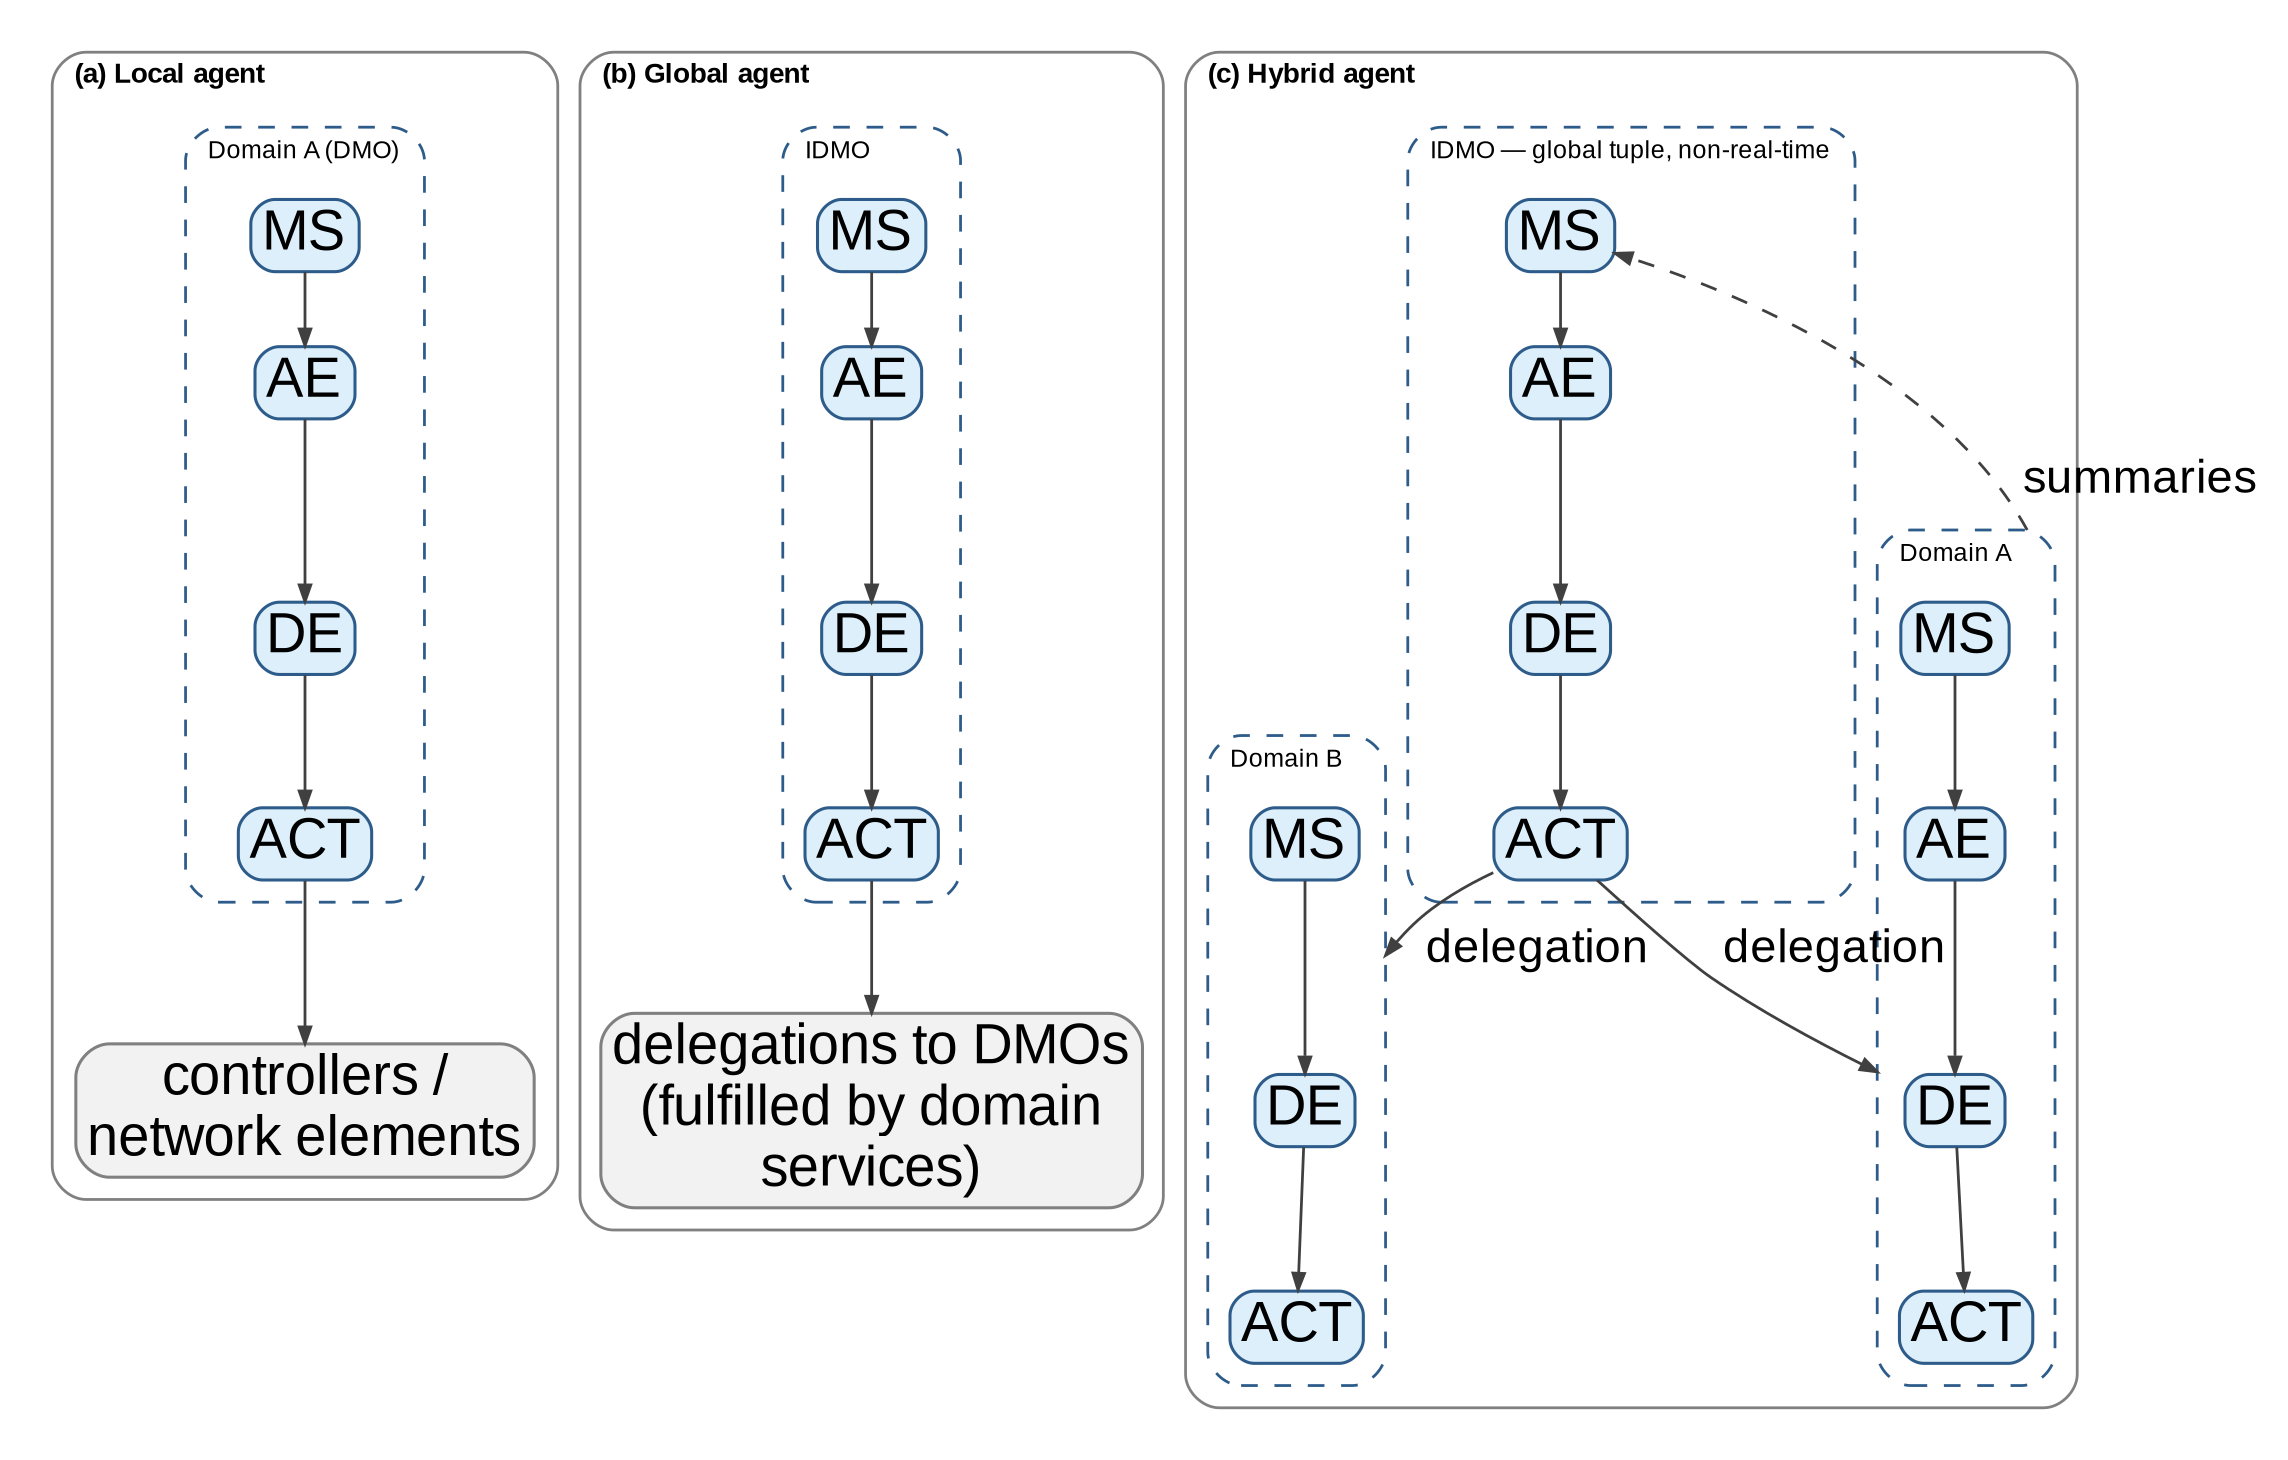
\includegraphics[width=\linewidth,height=0.45\textheight,keepaspectratio]{figures/image2.png}
\captionnum{3-2}
\caption{Local, global and hybrid agents}
\label{fig:3-2}
\end{figure}

\hypertarget{realization-patterns}{%
\subsubsection{Realization patterns}\label{realization-patterns}}

The DMO realizes a local agent according to one of five patterns, chosen
from the descriptor's capability modes, the delegation where the agent
realizes one, and the functions available in the domain's catalog:

\begin{itemize}
\tightlist
\item
  \emph{full tuple} --- MS, AE, DE and ACT deployed locally, for fast
  autonomous operation of the domain;
\item
  \emph{partial tuple} --- MS and ACT deployed locally, with AE and DE
  delegated to the agent's global agent, where global intelligence
  suffices and only local enforcement is needed;
\item
  \emph{reused services} --- an existing monitoring stack or controller
  bound as the provider of a delegated MS or ACT, with a new AE and DE
  deployed;
\item
  \emph{hierarchical local tuple} --- several MS instances, each
  observing part of a large or distributed domain, feeding one
  domain-level AE and DE;
\item
  \emph{advisory tuple} --- MS, AE and DE deployed with the agent held
  in the advisory authority state, so that actuation requires approval.
\end{itemize}

The descriptor constrains the choice of pattern through its capability
modes and its permitted binding classes, but does not name a pattern.
The pattern selected is recorded in the registry and in the resolved
configuration.

\hypertarget{contribution-classes}{%
\subsubsection{Contribution classes}\label{contribution-classes}}

Every partner contribution enters the platform as exactly one of four
classes, declared when it is registered in the catalog:

\begin{itemize}
\tightlist
\item
  \emph{role implementation} --- supplies the behavior of one or more
  capabilities of an agent, is described by an agent descriptor and is
  held to the full capability contracts. This is the ordinary case: for
  example the WP5 applications App-01 to App-04, App-06, App-07, App-09
  and App-12 to App-15, and the WP4 algorithms DPIR and RF-PLRE;
\item
  \emph{platform service} --- supplies a capability that the platform
  itself consumes and holds no role in any agent; it is held to its
  service contract. The conflict management service (App-10) and the
  trust modeling service (App-11) are platform services: the former is
  bound at the activation gate as the mediation endpoint and never
  mediates itself, and the latter enters at admission and registration
  and never on the per-decision path;
\item
  \emph{reused capability} --- an existing service bound as a provider
  rather than deployed, such as a monitoring stack, a model registry or
  a domain controller;
\item
  \emph{supporting application} --- operates alongside agents without
  holding a role in one, such as the XR application (App-05) or semantic
  domain switching offered as a service-level function (App-08).
\end{itemize}

Only role implementations are described by agent descriptors. The other
three classes are registered in the catalog with their service contracts
(Section 3.6) and may appear in a descriptor only as providers of
delegated capabilities or as endpoints of bindings.

\hypertarget{conformance-classes-and-the-extension-path}{%
\subsubsection{Conformance classes and the extension path}\label{conformance-classes-and-the-extension-path}}

A descriptor whose every declaration uses the normative schema and
catalog types is of normative conformance. A descriptor that contains an
extension field or references an extension type (Section 3.5.17) is of
extension conformance. The class is derived by the platform.

An extension agent enters at the advisory authority state. Its
containment is identical to that of a normative agent: the same egress
gate, the same mediation, the same stability enforcement, the same
rationale requirement and the same last-mile check apply. Freedom
applies to its algorithm, not to its guardrails. Sustained conformant
operation under evaluation is the route to promotion --- from advisory
to closed\_\allowbreak{}loop\_\allowbreak{}reduced and then to
closed\_\allowbreak{}loop\_\allowbreak{}full, under the criteria of
Chapter 9 --- and to the adoption of its extension types into the
catalog, after which the descriptor is republished at normative
conformance.

\hypertarget{technique-classes-and-admissibility}{%
\subsubsection{Technique classes and admissibility}\label{technique-classes-and-admissibility}}

Contributed logic declares its technique class per capability. The
technique changes no contract; it determines whether the logic is
admissible in a capability at all, and under which conditions (Table
3-11). A hybrid technique is subject to the conditions of every
technique it combines.

\begin{wptable}{3-11}

\begin{longtable}[]{@{}
  >{\raggedright\arraybackslash}p{(\columnwidth - 8\tabcolsep) * \real{0.1625}}
  >{\raggedright\arraybackslash}p{(\columnwidth - 8\tabcolsep) * \real{0.2094}}
  >{\raggedright\arraybackslash}p{(\columnwidth - 8\tabcolsep) * \real{0.2094}}
  >{\raggedright\arraybackslash}p{(\columnwidth - 8\tabcolsep) * \real{0.2094}}
  >{\raggedright\arraybackslash}p{(\columnwidth - 8\tabcolsep) * \real{0.2094}}@{}}
\caption{Admissibility of technique classes by
capability}\tabularnewline
\toprule\noalign{}
\begin{minipage}[b]{\linewidth}\raggedright
\textbf{Technique class}
\end{minipage} & \begin{minipage}[b]{\linewidth}\raggedright
\textbf{MS}
\end{minipage} & \begin{minipage}[b]{\linewidth}\raggedright
\textbf{AE}
\end{minipage} & \begin{minipage}[b]{\linewidth}\raggedright
\textbf{DE}
\end{minipage} & \begin{minipage}[b]{\linewidth}\raggedright
\textbf{ACT}
\end{minipage} \\
\midrule\noalign{}
\endfirsthead
\toprule\noalign{}
\begin{minipage}[b]{\linewidth}\raggedright
\textbf{Technique class}
\end{minipage} & \begin{minipage}[b]{\linewidth}\raggedright
\textbf{MS}
\end{minipage} & \begin{minipage}[b]{\linewidth}\raggedright
\textbf{AE}
\end{minipage} & \begin{minipage}[b]{\linewidth}\raggedright
\textbf{DE}
\end{minipage} & \begin{minipage}[b]{\linewidth}\raggedright
\textbf{ACT}
\end{minipage} \\
\midrule\noalign{}
\endhead
\bottomrule\noalign{}
\endlastfoot
\textbf{deterministic (rules, thresholds, state machines)} & Admissible
& Admissible & Admissible & Admissible; the default for translation \\
\textbf{optimization (solvers, bounded heuristics)} & Admissible for
acquisition control, such as adaptive sampling & Admissible &
Admissible; solutions are checked against the action space like any
proposal & Admissible only with deterministic execution: fixed seed and
bounded run time \\
\textbf{classical\_\allowbreak{}ml (supervised, unsupervised,
statistical)} & Admissible for acquisition functions only; never for
values presented as measured & Admissible with pinned model identity,
machine-evaluable validity conditions and drift signals & Admissible &
Not admissible \\
\textbf{reinforcement\_\allowbreak{}learning} & Not admissible &
Admissible as a predictor, under the AE conditions & Admissible;
exploration only through ordinary intents, subject to every bound;
weight updates follow the adaptation rule & Not admissible \\
\textbf{generative (based on language models, including tool use and
multi-step planning)} & Admissible as a query or observability
interface; output traceable to collected data and never presented as
measurement & Admissible with declared uncertainty and machine-evaluable
validity conditions & Admissible with output confined to the registered
action space; entry at advisory; declared read-only tools only & Not
admissible \\
\textbf{digital\_\allowbreak{}twin (simulation-based evaluation)} & Not
admissible: simulated values are not measurements & Admissible; insights
labeled as simulated & Admissible as evaluation within the decision;
twin validation confers no authority & Not admissible \\
\end{longtable}

\end{wptable}

Adaptation during operation is declared in the model hooks (Section
3.5.15). Adaptation that changes model weights produces a new model
identity and takes effect only through a generation-controlled update
performed by the DMO (Chapter 9); an agent never replaces its own model.
Adaptation that accumulates context without changing weights, as in
agents based on language models with episodic memory, is declared with a
bound on the retained context and the condition on which the context is
reset, and the agent's validity conditions and drift signals apply to it
unchanged.

\hypertarget{authority-ceilings-and-authority-states}{%
\subsubsection{Authority ceilings and authority states}\label{authority-ceilings-and-authority-states}}

The capabilities realized for an agent are those its descriptor
declares, and the composition class they form (Table 3-9) sets the first
of its authority ceilings; no service request selects them. A domain in
which no agent is instantiated runs without one, so an end-to-end
service may span agent-managed and conventionally managed domains
(Section 3.10).

The authority ceiling of an instance is the lowest of four ceilings:
that of its composition class, that permitted by the authority mode its
descriptor declares, that set by the interpretability of its decision
logic, and, for extension conformance until promotion, advisory.
Ceilings are ordered monitoring\_\allowbreak{}only, advisory,
closed\_\allowbreak{}loop\_\allowbreak{}reduced and
closed\_\allowbreak{}loop\_\allowbreak{}full, from lowest to highest.
The authority mode auto\_\allowbreak{}execute permits
closed\_\allowbreak{}loop\_\allowbreak{}full,
auto\_\allowbreak{}execute\_\allowbreak{}guarded permits
closed\_\allowbreak{}loop\_\allowbreak{}reduced, and
human\_\allowbreak{}approval\_\allowbreak{}required and advisory permit
advisory. Only agents of class closed\_\allowbreak{}loop declare an
authority mode. An instance whose descriptor does not declare its
decision logic interpretable, in the sense of Chapter 6, has a ceiling
of closed\_\allowbreak{}loop\_\allowbreak{}reduced; authority over the
network without an account of why an individual decision was taken is
the combination the framework does not permit.

Two of these modes carry a meaning wider than their names suggest, and
the framework fixes that meaning here. The mode advisory constrains the
agent, not its recipient: the agent never actuates, and what it emits is
a recommendation. The party that consumes the recommendation and decides
whether anything follows from it is outside the agent and outside the
descriptor --- a human approver registered for the domain, another
agent, a supervising service, or an operator-facing tool through which a
person acts. That consumption may be iterative: recommendations arrive
over successive cycles and the consumer may act on none of them, on one,
or on a sequence. The descriptor therefore declares neither the identity
nor the class of the consumer, and the framework places no requirement
on it beyond those of Section 3.5.10 for the contract on which
recommendations are published.

The mode auto\_\allowbreak{}execute\_\allowbreak{}guarded permits the
agent to close the loop, subject to a guard that is external to the
agent. A guard is any mechanism that may withhold, bound or reverse what
the agent proposes and that the agent does not itself implement: a human
in the loop at one end of the range, an automatic guardrail --- a rule
engine, a safety monitor, a supervisory policy function --- at the
other. The framework requires that such a mechanism be in place for this
mode and that its decisions be recorded in the agent's rationale and in
assurance; it does not require that the guard reside in any particular
place in the architecture, and the descriptor does not name it. Where
the guard is a registered approver, the agent behaves as in the advisory
authority state for the actions the guard holds.

An agent instance occupies exactly one of the seven authority states of
Table 3-12 at any time. The state is held in the registry --- by the DMO
for local agents and by the IDMO for global agents --- and is consulted
by the capability runtimes every cycle. Promotion requires the
activation gate; demotion is automatic on the thresholds declared for it
and requires no human step. Every transition is a lifecycle event and is
reported in assurance. The transitions are specified in Chapter 9.

\begin{wptable}{3-12}

\begin{longtable}[]{@{}
  >{\raggedright\arraybackslash}p{(\columnwidth - 6\tabcolsep) * \real{0.2438}}
  >{\raggedright\arraybackslash}p{(\columnwidth - 6\tabcolsep) * \real{0.2375}}
  >{\raggedright\arraybackslash}p{(\columnwidth - 6\tabcolsep) * \real{0.2000}}
  >{\raggedright\arraybackslash}p{(\columnwidth - 6\tabcolsep) * \real{0.3187}}@{}}
\caption{Authority states}\tabularnewline
\toprule\noalign{}
\begin{minipage}[b]{\linewidth}\raggedright
\textbf{State}
\end{minipage} & \begin{minipage}[b]{\linewidth}\raggedright
\textbf{Decision emission}
\end{minipage} & \begin{minipage}[b]{\linewidth}\raggedright
\textbf{Actuation}
\end{minipage} & \begin{minipage}[b]{\linewidth}\raggedright
\textbf{Entered on}
\end{minipage} \\
\midrule\noalign{}
\endfirsthead
\toprule\noalign{}
\begin{minipage}[b]{\linewidth}\raggedright
\textbf{State}
\end{minipage} & \begin{minipage}[b]{\linewidth}\raggedright
\textbf{Decision emission}
\end{minipage} & \begin{minipage}[b]{\linewidth}\raggedright
\textbf{Actuation}
\end{minipage} & \begin{minipage}[b]{\linewidth}\raggedright
\textbf{Entered on}
\end{minipage} \\
\midrule\noalign{}
\endhead
\bottomrule\noalign{}
\endlastfoot
\textbf{admitted\_\allowbreak{}not\_\allowbreak{}active} & None &
Inhibited; dry run only, during the activation gate & Admission passed;
activation gate not yet satisfied \\
\textbf{monitoring\_\allowbreak{}only} & DE not invoked & Inhibited &
Ceiling monitoring\_\allowbreak{}only; gate outcome observation-only;
demotion \\
\textbf{advisory} & Intents published as recommendations; an approved
recommendation proceeds as an intent carrying the approval reference &
Approved intents only, after mediation & Extension conformance; ceiling
advisory; gate outcome advisory; demotion \\
\textbf{closed\_\allowbreak{}loop\_\allowbreak{}reduced} & Intents
within a narrowed control scope, tightened bounds and a lower priority
band & Active & Gate outcome restricted; demotion by evaluation \\
\textbf{closed\_\allowbreak{}loop\_\allowbreak{}full} & Intents within
the full granted authority & Active & Gate passed at full authority \\
\textbf{suspended} & Withdrawn & Inhibited, except completion of
verification and permitted rollback of transactions already in flight &
Binding fault; orchestration-initiated migration or termination;
operator intervention; loss of the mediation binding, at the expiry of
any action envelope then held; evaluation \\
\textbf{terminated} & None & None & Termination; generation retired \\
\end{longtable}

\end{wptable}

In the advisory state a recommendation becomes an intent only when an
approver registered for the domain approves it, and never where the
descriptor declares the authority mode advisory --- in which case the
recommendation leaves the platform through its published contract and
any action that follows is taken outside the agent's authority. The
approved intent is then mediated, bounded and executed exactly as any
other intent, and carries the approval reference in its rationale.
Independently of the state, an action type declared unverifiable
executes only under the restrictions of Section 3.5.8.

\hypertarget{the-agent-descriptor}{%
\subsection{The Agent Descriptor}\label{the-agent-descriptor}}

\hypertarget{the-descriptor-chain}{%
\subsubsection{The descriptor chain}\label{the-descriptor-chain}}

An agent passes through three documents between its conception and its
operation (Figure 3-3). The \emph{functional specification} is written
by the contributor and states in natural language what the agent is for:
its objective, the evidence it needs, the decisions it takes, the
actions it may request and how it behaves when conditions degrade. It
follows the project's tuple specification template, which records the
loop's objectives and, for each capability, its role, placement, inputs,
processing, outputs, configurable parameters and non-functional
requirements. The \emph{agent descriptor} is compiled from the
functional specification into the machine-readable, versioned and signed
contract that the platform acts upon, and is registered in the catalog.
The \emph{service tree}, carried in the descriptor itself, declares the
services each tuple requires and is resolved by the orchestrator the
descriptor is issued to: the IDMO where the agent is global, which
resolves the tree into one portion per domain, and the domain's DMO
where it is local. The \emph{resolved configuration} is returned by the
DMO after realization and records the identifiers, endpoints and
bindings of the instance and the state in which it was admitted.

Each document is owned by a different party --- the contributor, the
catalog and the DMO --- and each later document may narrow what an
earlier one allows but never widen it: the scope of an instance is
contained in the scope of its descriptor, and the authority granted to
an instance does not exceed the authority its descriptor declares. The
functional specification is not checked by the platform; only the
descriptor and the documents that follow it are acted upon.

\begin{figure}[htbp]
\centering
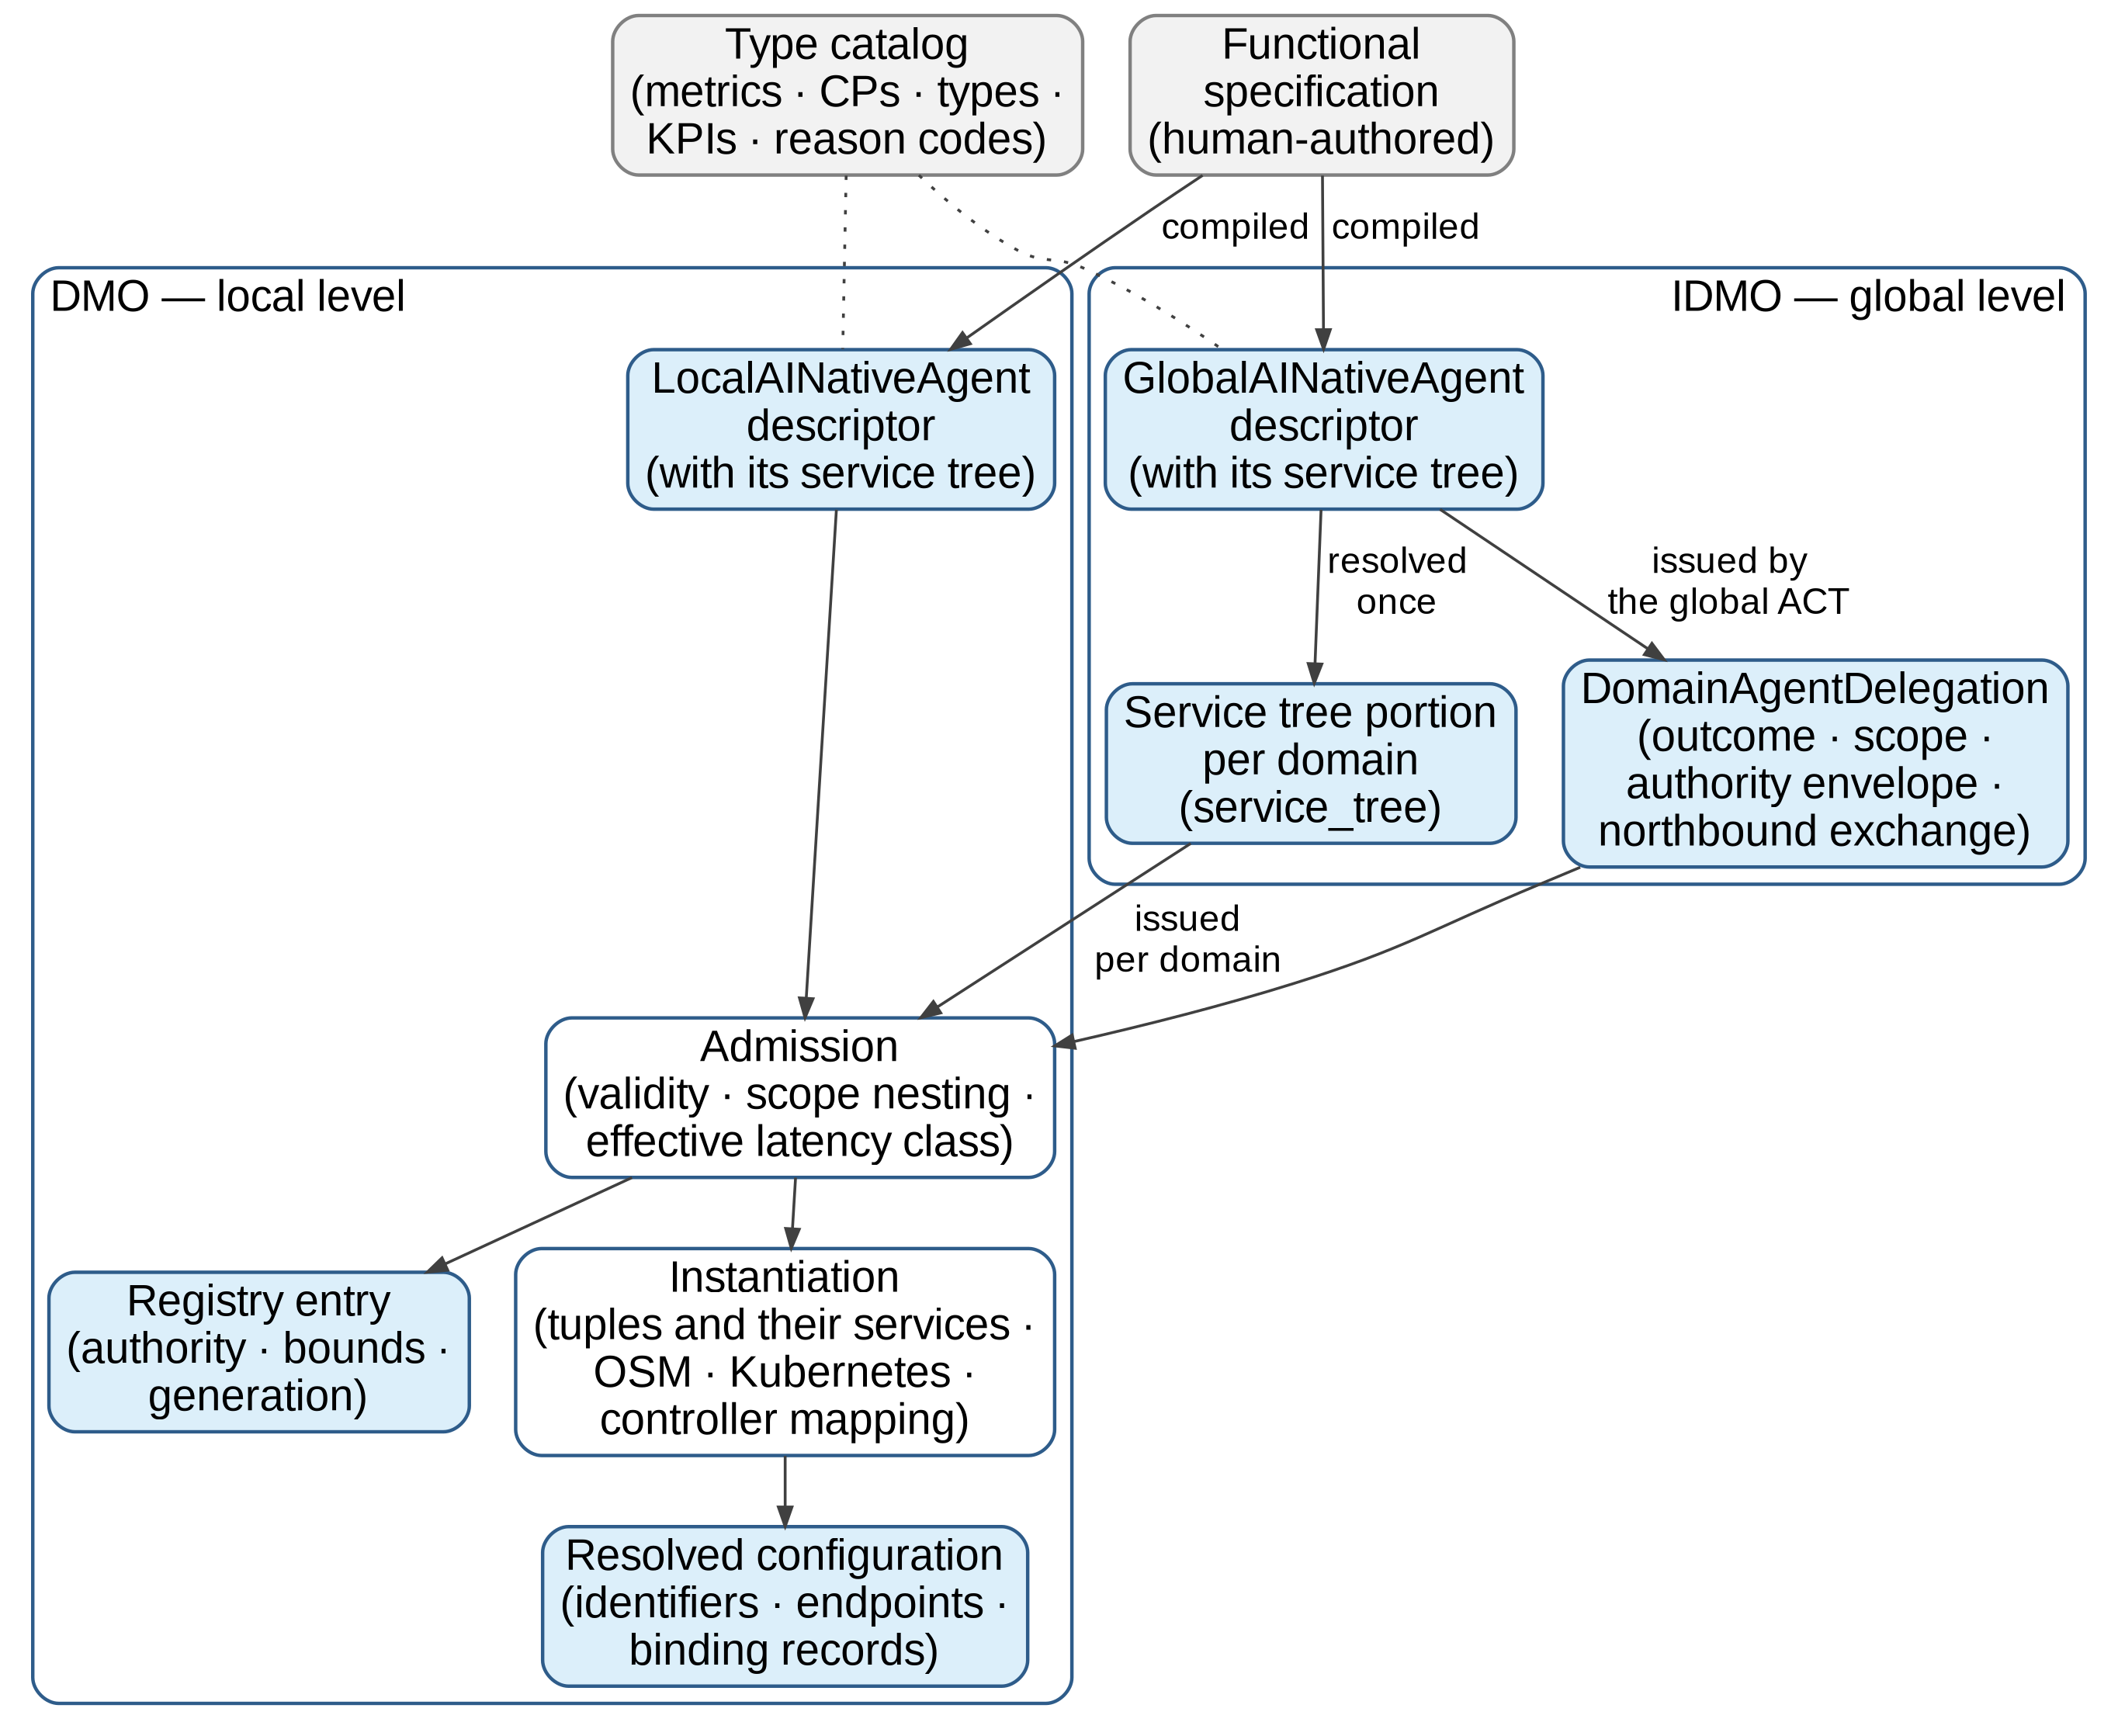
\includegraphics[width=\linewidth,height=0.45\textheight,keepaspectratio]{figures/image3.png}
\captionnum{3-3}
\caption{The descriptor chain at the global and local levels}
\label{fig:3-3}
\end{figure}

\hypertarget{descriptor-levels}{%
\subsubsection{Descriptor levels}\label{descriptor-levels}}

Agents are described at two levels. A LocalAINativeAgent descriptor,
owned by a DMO, describes a local agent and is specified field by field
in Sections 3.5.3 to 3.5.20. A GlobalAINativeAgent descriptor, owned by
the IDMO, describes a global agent and follows the same structure, with
four differences: its only domain is the IDMO; the controller binding of
its ACT is the IDMO's delegation interface towards the DMOs; its action
space consists of delegation operations --- create, update, approve,
suspend and terminate a delegation, and issue an intent to a DMO; and
its physical deployment addresses hosting at the IDMO only. A global
descriptor contains no domain-internal placement, network service
descriptor or controller mapping.

A third document, the DomainAgentDelegation, is not an agent descriptor.
It is the document by which the ACT of a global agent assigns an
outcome-oriented responsibility to one domain (Section 3.5.21).
Deployment translation --- to OSM, Kubernetes, Helm or controller
mappings --- belongs to the DMO and never appears in a global descriptor
or in a delegation.

\hypertarget{document-structure}{%
\subsubsection{Document structure}\label{document-structure}}

An agent descriptor consists of the sections of Table 3-13. The
applicability of each section depends on the composition class that the
platform derives from the tuple section. In the table, CL, OL, AN, OB
and AS denote the composition classes closed\_\allowbreak{}loop,
open\_\allowbreak{}loop, analytics, observation and
actuation\_\allowbreak{}service; M marks a mandatory section, C a
section required under the condition stated in its own table, O an
optional section, and a dash a section that shall be absent.

\begin{wptable}{3-13}\footnotesize

\begin{longtable}[]{@{}
  >{\raggedright\arraybackslash}p{(\columnwidth - 12\tabcolsep) * \real{0.2875}}
  >{\raggedright\arraybackslash}p{(\columnwidth - 12\tabcolsep) * \real{0.3375}}
  >{\raggedright\arraybackslash}p{(\columnwidth - 12\tabcolsep) * \real{0.0750}}
  >{\raggedright\arraybackslash}p{(\columnwidth - 12\tabcolsep) * \real{0.0750}}
  >{\raggedright\arraybackslash}p{(\columnwidth - 12\tabcolsep) * \real{0.0750}}
  >{\raggedright\arraybackslash}p{(\columnwidth - 12\tabcolsep) * \real{0.0750}}
  >{\raggedright\arraybackslash}p{(\columnwidth - 12\tabcolsep) * \real{0.0751}}@{}}
\caption{Sections of the agent descriptor}\tabularnewline
\toprule\noalign{}
\begin{minipage}[b]{\linewidth}\raggedright
\textbf{Section}
\end{minipage} & \begin{minipage}[b]{\linewidth}\raggedright
\textbf{Content}
\end{minipage} & \begin{minipage}[b]{\linewidth}\raggedright
\textbf{CL}
\end{minipage} & \begin{minipage}[b]{\linewidth}\raggedright
\textbf{OL}
\end{minipage} & \begin{minipage}[b]{\linewidth}\raggedright
\textbf{AN}
\end{minipage} & \begin{minipage}[b]{\linewidth}\raggedright
\textbf{OB}
\end{minipage} & \begin{minipage}[b]{\linewidth}\raggedright
\textbf{AS}
\end{minipage} \\
\midrule\noalign{}
\endfirsthead
\toprule\noalign{}
\begin{minipage}[b]{\linewidth}\raggedright
\textbf{Section}
\end{minipage} & \begin{minipage}[b]{\linewidth}\raggedright
\textbf{Content}
\end{minipage} & \begin{minipage}[b]{\linewidth}\raggedright
\textbf{CL}
\end{minipage} & \begin{minipage}[b]{\linewidth}\raggedright
\textbf{OL}
\end{minipage} & \begin{minipage}[b]{\linewidth}\raggedright
\textbf{AN}
\end{minipage} & \begin{minipage}[b]{\linewidth}\raggedright
\textbf{OB}
\end{minipage} & \begin{minipage}[b]{\linewidth}\raggedright
\textbf{AS}
\end{minipage} \\
\midrule\noalign{}
\endhead
\bottomrule\noalign{}
\endlastfoot
\textbf{schema\_\allowbreak{}version, kind} & Schema version;
LocalAINativeAgent or GlobalAINativeAgent & M & M & M & M & M \\
\textbf{identity} & Identity and publisher (Table 3-14) & M & M & M & M
& M \\
\textbf{tuple\_\allowbreak{}capabilities,
capability\_\allowbreak{}subsets, capability\_\allowbreak{}delegations}
& Capability modes, subsets and delegations (Table 3-15) & M & M & M & M
& M \\
\textbf{objectives} & Objective templates (Table 3-16) & M & M & --- &
--- & --- \\
\textbf{scope} & Primary and secondary domains, scope selectors,
observation and control scope (Table 3-17) & M & M & M & M & M \\
\textbf{action\_\allowbreak{}space} & Action types and their bounds
(Table 3-18) & M & M & --- & --- & M \\
\textbf{functions} & Per-capability function declarations (Tables 3-19
to 3-22) & M & M & M & M & M \\
\textbf{interfaces} & Flows, schemas, permitted bindings, exposed
contracts (Table 3-23) & M & M & M & M & M \\
\textbf{operations} & Operating mode, latency class, loop budget,
declared latencies (Table 3-24) & M & M & M & M & M \\
\textbf{physical\_\allowbreak{}deployment} & Allowed tiers, locations,
affinity, resources, state, artifacts, split deployment, migration
(Table 3-25) & M & M & M & M & M \\
\textbf{policies} & Authority mode, conflict resolution, priority,
mediation requests (Table 3-26) & M & --- & --- & --- & --- \\
\textbf{failure\_\allowbreak{}policy} & Per-capability failure behavior
(Table 3-27) & M & M & M & M & M \\
\textbf{model\_\allowbreak{}hooks} & Model artifacts, update policy,
drift signals, fallback (Table 3-28) & C & C & C & C & --- \\
\textbf{ownership, integrity} & Owner, stakeholder role, trust domain,
hash, signature, SBOM, platform dependencies (Table 3-29) & M & M & M &
M & M \\
\textbf{service\_\allowbreak{}tree} & Services required per tuple, tuple
bindings, domains of a global agent, operational timeout (Table 3-31) &
M & M & M & M & M \\
\textbf{x-*} & Extension fields (Section 3.5.17) & O & O & O & O & O \\
\end{longtable}

\end{wptable}

\hypertarget{identity}{%
\subsubsection{Identity}\label{identity}}

\begin{wptable}{3-14}

\begin{longtable}[]{@{}
  >{\raggedright\arraybackslash}p{(\columnwidth - 6\tabcolsep) * \real{0.2875}}
  >{\raggedright\arraybackslash}p{(\columnwidth - 6\tabcolsep) * \real{0.1438}}
  >{\raggedright\arraybackslash}p{(\columnwidth - 6\tabcolsep) * \real{0.0750}}
  >{\raggedright\arraybackslash}p{(\columnwidth - 6\tabcolsep) * \real{0.4937}}@{}}
\caption{Identity fields}\tabularnewline
\toprule\noalign{}
\begin{minipage}[b]{\linewidth}\raggedright
\textbf{Field}
\end{minipage} & \begin{minipage}[b]{\linewidth}\raggedright
\textbf{Type}
\end{minipage} & \begin{minipage}[b]{\linewidth}\raggedright
\textbf{Req.}
\end{minipage} & \begin{minipage}[b]{\linewidth}\raggedright
\textbf{Semantics and constraints}
\end{minipage} \\
\midrule\noalign{}
\endfirsthead
\toprule\noalign{}
\begin{minipage}[b]{\linewidth}\raggedright
\textbf{Field}
\end{minipage} & \begin{minipage}[b]{\linewidth}\raggedright
\textbf{Type}
\end{minipage} & \begin{minipage}[b]{\linewidth}\raggedright
\textbf{Req.}
\end{minipage} & \begin{minipage}[b]{\linewidth}\raggedright
\textbf{Semantics and constraints}
\end{minipage} \\
\midrule\noalign{}
\endhead
\bottomrule\noalign{}
\endlastfoot
\textbf{schema\_\allowbreak{}version} & semver & M & Version of the
descriptor schema; one of the versions the registry lists as
supported. \\
\textbf{kind} & enum & M & LocalAINativeAgent or GlobalAINativeAgent. \\
\textbf{identity.\allowbreak{}descriptor\_\allowbreak{}id} & id & M &
Stable URN of the agent type (Table 3-2). \\
\textbf{identity.\allowbreak{}version} & semver & M & Version of this
descriptor (Section 3.5.19). \\
\textbf{identity.\allowbreak{}agent\_\allowbreak{}version} & string & O
& Release identifier of the contributed logic, with build metadata;
informative, the artifact digests being authoritative. \\
\textbf{identity.name} & string & M & Human-readable name of at most 64
characters. \\
\textbf{identity.\allowbreak{}publisher\_\allowbreak{}identity} & string
& M & Organization contributing the agent, with its support channel;
resolves to a signing key in the agent\textquotesingle s trust
domain. \\
\textbf{identity.\allowbreak{}functional\_\allowbreak{}specification\_\allowbreak{}ref}
& string & O & Reference to the functional specification from which the
descriptor was compiled. \\
\textbf{identity.\allowbreak{}description} & string & O & Informative
text; not interpreted by the platform. \\
\textbf{identity.\allowbreak{}labels} & map & O & Discovery labels; not
interpreted by the platform. \\
\textbf{identity.\allowbreak{}license\_\allowbreak{}and\_\allowbreak{}ip}
& object & O & Licensing declaration: an SPDX license expression or
proprietary, and whether the artifacts are subject to export control;
not interpreted by admission. \\
\end{longtable}

\end{wptable}

\hypertarget{tuple-declaration-and-delegations}{%
\subsubsection{Tuple declaration and delegations}\label{tuple-declaration-and-delegations}}

The tuple sections declare the mode of each capability, the enumerated
subset of each partial capability and the provider of each delegated
capability (Table 3-15). The capability keys are MS, AE, DE and ACT.

\begin{wptable}{3-15}

\begin{longtable}[]{@{}
  >{\raggedright\arraybackslash}p{(\columnwidth - 6\tabcolsep) * \real{0.2875}}
  >{\raggedright\arraybackslash}p{(\columnwidth - 6\tabcolsep) * \real{0.1438}}
  >{\raggedright\arraybackslash}p{(\columnwidth - 6\tabcolsep) * \real{0.0750}}
  >{\raggedright\arraybackslash}p{(\columnwidth - 6\tabcolsep) * \real{0.4937}}@{}}
\caption{Tuple fields}\tabularnewline
\toprule\noalign{}
\begin{minipage}[b]{\linewidth}\raggedright
\textbf{Field}
\end{minipage} & \begin{minipage}[b]{\linewidth}\raggedright
\textbf{Type}
\end{minipage} & \begin{minipage}[b]{\linewidth}\raggedright
\textbf{Req.}
\end{minipage} & \begin{minipage}[b]{\linewidth}\raggedright
\textbf{Semantics and constraints}
\end{minipage} \\
\midrule\noalign{}
\endfirsthead
\toprule\noalign{}
\begin{minipage}[b]{\linewidth}\raggedright
\textbf{Field}
\end{minipage} & \begin{minipage}[b]{\linewidth}\raggedright
\textbf{Type}
\end{minipage} & \begin{minipage}[b]{\linewidth}\raggedright
\textbf{Req.}
\end{minipage} & \begin{minipage}[b]{\linewidth}\raggedright
\textbf{Semantics and constraints}
\end{minipage} \\
\midrule\noalign{}
\endhead
\bottomrule\noalign{}
\endlastfoot
\textbf{tuple\_\allowbreak{}capabilities.\allowbreak{}\textless cap\textgreater{}}
& enum & M & full, partial, delegated or none, for each of MS, AE, DE
and ACT. \\
\textbf{capability\_\allowbreak{}subsets.\allowbreak{}\textless cap\textgreater{}}
& list of type-ref & C & Required where the mode is partial. MS: metrics
or managed-object classes of the observation scope. AE: insight types.
DE: action types forming the decision space. ACT: action types
executed. \\
\textbf{capability\_\allowbreak{}delegations.\allowbreak{}\textless cap\textgreater.\allowbreak{}provider}
& id & C & Required where the mode is delegated, or the complement of a
partial subset is delegated. descriptor\_\allowbreak{}id of a provider
agent, or catalog identifier of a platform service or reused
capability. \\
\textbf{capability\_\allowbreak{}delegations.\allowbreak{}\textless cap\textgreater.\allowbreak{}covers}
& enum & C & Required where a provider is declared. all, where the
capability is delegated; complement, where the delegation covers the
complement of a partial subset. \\
\textbf{capability\_\allowbreak{}delegations.\allowbreak{}\textless cap\textgreater.\allowbreak{}interface}
& type-ref & C & Required where a provider is declared. Service contract
exposed by the provider. \\
\textbf{capability\_\allowbreak{}delegations.\allowbreak{}\textless cap\textgreater.\allowbreak{}interface\_\allowbreak{}profile}
& type-ref & C & Required where a provider is declared. Pinned interface
profile of the provider. \\
\textbf{capability\_\allowbreak{}delegations.\allowbreak{}\textless cap\textgreater.\allowbreak{}compatibility}
& semver-range & C & Required where a provider is declared. Accepted
provider versions; for a delegated AE, also the accepted model
versions. \\
\textbf{capability\_\allowbreak{}delegations.\allowbreak{}\textless cap\textgreater.\allowbreak{}sla\_\allowbreak{}assumptions}
& object & C & Required where a provider is declared. Maximum
99th-percentile latency and maximum age at delivery that the consumer
assumes of the provider; admission rejects a provider whose declared
figures exceed them. \\
\end{longtable}

\end{wptable}

A delegation pins the provider's interface profile and a range of
accepted provider versions. At admission the provider's declared scope
shall cover the consumer's, and the provider's declared latency and
freshness shall be within the consumer's SLA assumptions. At runtime the
provider's health and coverage are forwarded to the consumer as part of
the binding, and a provider whose published interface profile or version
leaves the pinned range raises a binding fault at the consumer, which
suspends the affected capability. A delegated ACT provider shall itself
satisfy every requirement on the ACT (Chapter 7).

\hypertarget{objectives}{%
\subsubsection{Objectives}\label{objectives}}

Objectives are declared as templates over KPIs of the catalog (Table
3-16). The target values of templates marked as bound by the request are
supplied when the descriptor is issued for instantiation, once, and are
fixed for the life of the instance; a change of target values is a new
agent (Section 3.5.20). At admission the platform registers the KPIs of
an agent's objectives with the conflict fabric as the KPI side of the
agent's registration (Chapter 10).

\begin{wptable}{3-16}

\begin{longtable}[]{@{}
  >{\raggedright\arraybackslash}p{(\columnwidth - 6\tabcolsep) * \real{0.2875}}
  >{\raggedright\arraybackslash}p{(\columnwidth - 6\tabcolsep) * \real{0.1438}}
  >{\raggedright\arraybackslash}p{(\columnwidth - 6\tabcolsep) * \real{0.0750}}
  >{\raggedright\arraybackslash}p{(\columnwidth - 6\tabcolsep) * \real{0.4937}}@{}}
\caption{Objective fields}\tabularnewline
\toprule\noalign{}
\begin{minipage}[b]{\linewidth}\raggedright
\textbf{Field in objectives{[}{]}}
\end{minipage} & \begin{minipage}[b]{\linewidth}\raggedright
\textbf{Type}
\end{minipage} & \begin{minipage}[b]{\linewidth}\raggedright
\textbf{Req.}
\end{minipage} & \begin{minipage}[b]{\linewidth}\raggedright
\textbf{Semantics and constraints}
\end{minipage} \\
\midrule\noalign{}
\endfirsthead
\toprule\noalign{}
\begin{minipage}[b]{\linewidth}\raggedright
\textbf{Field in objectives{[}{]}}
\end{minipage} & \begin{minipage}[b]{\linewidth}\raggedright
\textbf{Type}
\end{minipage} & \begin{minipage}[b]{\linewidth}\raggedright
\textbf{Req.}
\end{minipage} & \begin{minipage}[b]{\linewidth}\raggedright
\textbf{Semantics and constraints}
\end{minipage} \\
\midrule\noalign{}
\endhead
\bottomrule\noalign{}
\endlastfoot
\textbf{objective\_\allowbreak{}id} & string & M & Unique within the
descriptor. \\
\textbf{kpi} & type-ref & M & Objective KPI of the catalog, with its
unit and measurement methodology. \\
\textbf{direction} & enum & M & minimize, maximize,
hold\_\allowbreak{}below, hold\_\allowbreak{}above or
hold\_\allowbreak{}within.\allowbreak{} \\
\textbf{target} & object & M & from\_\allowbreak{}request, bound when
the descriptor is issued for instantiation; or a fixed value in the
KPI\textquotesingle s unit --- a pair of values for
hold\_\allowbreak{}within.\allowbreak{} \\
\textbf{evaluation\_\allowbreak{}window} & duration & M & Window over
which objective status is evaluated for assurance. \\
\textbf{at\_\allowbreak{}risk\_\allowbreak{}margin} & ratio & M &
Fraction of the target within which the status is at-risk rather than
met. \\
\textbf{rank} & integer & O & Order among the agent\textquotesingle s
own objectives, 1 highest; used by its DE only, with no effect on
arbitration priority. \\
\end{longtable}

\end{wptable}

Objective status is evaluated over the evaluation window. For a
hold\_\allowbreak{}below objective with target T and at-risk margin m,
the status is \emph{met} while the KPI does not exceed T(1 − m),
\emph{at-risk} while it lies above T(1 − m) and at most T, and
\emph{not-met} above T. A hold\_\allowbreak{}above objective is
evaluated symmetrically, and a hold\_\allowbreak{}within objective
applies both conditions to its two targets. A minimize or maximize
objective with a target is evaluated as hold\_\allowbreak{}below or
hold\_\allowbreak{}above respectively; without a target it has no status
and serves only the agent's own DE.

\hypertarget{scope}{%
\subsubsection{Scope}\label{scope}}

\begin{wptable}{3-17}

\begin{longtable}[]{@{}
  >{\raggedright\arraybackslash}p{(\columnwidth - 6\tabcolsep) * \real{0.2875}}
  >{\raggedright\arraybackslash}p{(\columnwidth - 6\tabcolsep) * \real{0.1438}}
  >{\raggedright\arraybackslash}p{(\columnwidth - 6\tabcolsep) * \real{0.0750}}
  >{\raggedright\arraybackslash}p{(\columnwidth - 6\tabcolsep) * \real{0.4937}}@{}}
\caption{Scope fields}\tabularnewline
\toprule\noalign{}
\begin{minipage}[b]{\linewidth}\raggedright
\textbf{Field in scope}
\end{minipage} & \begin{minipage}[b]{\linewidth}\raggedright
\textbf{Type}
\end{minipage} & \begin{minipage}[b]{\linewidth}\raggedright
\textbf{Req.}
\end{minipage} & \begin{minipage}[b]{\linewidth}\raggedright
\textbf{Semantics and constraints}
\end{minipage} \\
\midrule\noalign{}
\endfirsthead
\toprule\noalign{}
\begin{minipage}[b]{\linewidth}\raggedright
\textbf{Field in scope}
\end{minipage} & \begin{minipage}[b]{\linewidth}\raggedright
\textbf{Type}
\end{minipage} & \begin{minipage}[b]{\linewidth}\raggedright
\textbf{Req.}
\end{minipage} & \begin{minipage}[b]{\linewidth}\raggedright
\textbf{Semantics and constraints}
\end{minipage} \\
\midrule\noalign{}
\endhead
\bottomrule\noalign{}
\endlastfoot
\textbf{primary\_\allowbreak{}domain} & enum & M & Domain of Table 3-10
in which the agent observes and acts; idmo for a global agent. \\
\textbf{secondary\_\allowbreak{}domains} & list of enum & C & Required
where a delegation crosses a domain boundary. Domains of the providers
of the agent\textquotesingle s cross-domain delegations (Section 3.3.5),
listed exactly: the domains of AE providers, and idmo where the DE is
delegated to the agent\textquotesingle s global agent. They are never
part of the control scope. \\
\textbf{scope\_\allowbreak{}selectors} & list of enum & M & Selector
dimensions in which the concrete scope of an instance is expressed and
which every message carries as scope tags: any of region, site, slice,
tenant and technology. \\
\textbf{observation\_\allowbreak{}scope.\allowbreak{}object\_\allowbreak{}classes}
& list of enum & C & Required where the MS or the AE is not none.
Managed-object classes observed: node, link, path, slice, flow, service,
ue, device; delegation for a global agent. \\
\textbf{observation\_\allowbreak{}scope.\allowbreak{}metrics} & list of
type-ref & C & Required where the MS is not none. Catalog metrics
observed. \\
\textbf{control\_\allowbreak{}scope.\allowbreak{}object\_\allowbreak{}classes}
& list of enum & C & Required where the DE or the ACT is not none.
Managed-object classes whose parameters may change. \\
\textbf{control\_\allowbreak{}scope.\allowbreak{}control\_\allowbreak{}parameters}
& list of type-ref & C & Required where the DE or the ACT is not none.
Catalog control parameters that may change. \\
\textbf{max\_\allowbreak{}objects} & integer & O & Upper bound on the
number of managed objects an instance may be granted; admission rejects
an instantiation that exceeds it. \\
\end{longtable}

\end{wptable}

Scopes nest. For every agent the control scope shall be contained in the
observation-justified scope, which shall be contained in the declared
domain scope, which shall be contained in the agent's trust domain. The
observation-justified scope comprises the managed-object classes for
which the agent's evidence --- its own MS, or a delegated MS or AE ---
includes at least one metric: an agent shall not change what it cannot
observe. At instantiation the declared scopes are bound to concrete
identifiers, once, and the same nesting shall hold for those
identifiers.

\hypertarget{action-space}{%
\subsubsection{Action space}\label{action-space}}

The action space is the set of actions the agent may request. It is the
object on which most of the framework's bounds act: the egress gate of
the DE, the registration with the conflict fabric, the last-mile check
of the ACT and the platform's stability enforcement all apply to it.
Each action type of the catalog that the agent may request appears once
in the action space, with the attributes of Table 3-18.

\begin{wptable}{3-18}

\begin{longtable}[]{@{}
  >{\raggedright\arraybackslash}p{(\columnwidth - 6\tabcolsep) * \real{0.2875}}
  >{\raggedright\arraybackslash}p{(\columnwidth - 6\tabcolsep) * \real{0.1438}}
  >{\raggedright\arraybackslash}p{(\columnwidth - 6\tabcolsep) * \real{0.0750}}
  >{\raggedright\arraybackslash}p{(\columnwidth - 6\tabcolsep) * \real{0.4937}}@{}}
\caption{Action space fields, per action type}\tabularnewline
\toprule\noalign{}
\begin{minipage}[b]{\linewidth}\raggedright
\textbf{Field}
\end{minipage} & \begin{minipage}[b]{\linewidth}\raggedright
\textbf{Type}
\end{minipage} & \begin{minipage}[b]{\linewidth}\raggedright
\textbf{Req.}
\end{minipage} & \begin{minipage}[b]{\linewidth}\raggedright
\textbf{Semantics and constraints}
\end{minipage} \\
\midrule\noalign{}
\endfirsthead
\toprule\noalign{}
\begin{minipage}[b]{\linewidth}\raggedright
\textbf{Field}
\end{minipage} & \begin{minipage}[b]{\linewidth}\raggedright
\textbf{Type}
\end{minipage} & \begin{minipage}[b]{\linewidth}\raggedright
\textbf{Req.}
\end{minipage} & \begin{minipage}[b]{\linewidth}\raggedright
\textbf{Semantics and constraints}
\end{minipage} \\
\midrule\noalign{}
\endhead
\bottomrule\noalign{}
\endlastfoot
\textbf{action\_\allowbreak{}type} & type-ref & M & Catalog action
type. \\
\textbf{targets} & object & M & Managed-object class and control
parameters changed; contained in the control scope. \\
\textbf{parameter\_\allowbreak{}bounds} & map & M & For each parameter:
minimum, maximum and step, or an enumeration of permitted values. \\
\textbf{rate\_\allowbreak{}limit} & rate & M & Maximum number of
executions per target. \\
\textbf{stability.\allowbreak{}cooldown} & duration & M & Minimum
interval between two executions on the same target. \\
\textbf{stability.\allowbreak{}minimum\_\allowbreak{}hold\_\allowbreak{}time}
& duration & M & Minimum time a change remains in effect on a target
before an execution that reverses it. \\
\textbf{stability.\allowbreak{}max\_\allowbreak{}step} & map & O &
Maximum change of each parameter in one execution. \\
\textbf{stability.\allowbreak{}staging} & list & O & Ordered stages,
each with a fraction of the targets and a dwell time, for changes
applied progressively. \\
\textbf{preconditions} & list of predicate & O & Conditions on the state
of the target, evaluated by the ACT runtime before submission. \\
\textbf{verification.\allowbreak{}method} & enum & M &
ms\_\allowbreak{}observation,
controller\_\allowbreak{}state\_\allowbreak{}query or unverifiable. \\
\textbf{verification.\allowbreak{}timing} & enum & C & Required where
the method is not unverifiable. in\_\allowbreak{}band or deferred. \\
\textbf{verification.\allowbreak{}deadline} & duration & C & Required
where the timing is deferred. Deadline within which deferred
verification completes. \\
\textbf{idempotency} & enum & M & idempotent or
non\_\allowbreak{}idempotent.\allowbreak{} \\
\textbf{rollback} & enum & M & supported, using the rollback method of
the catalog entry; or not\_\allowbreak{}supported.\allowbreak{} \\
\textbf{mediation\_\allowbreak{}path} & enum & M & envelope, policy or
mediated: the path by which the action is expected to be authorized
(Section 3.9.2). \\
\end{longtable}

\end{wptable}

An action type whose effect cannot be verified through a path
independent of the controller's acknowledgement is declared with the
verification method unverifiable. Such an action type is admitted only
with targets enumerated individually at instantiation rather than by
class, with a rate limit no higher than the ceiling for unverifiable
execution that its catalog entry sets, with every execution reported to
the DMO as it occurs, and under elevated evaluation scrutiny. These
restrictions bound where and how often such an action is taken; they do
not lower the authority of the agent that takes it, and an agent at
closed\_\allowbreak{}loop\_\allowbreak{}full executes an unverifiable
action type within them without approval. Its outcome is never
ACKNOWLEDGED\_\allowbreak{}VERIFIED.\allowbreak{}

\hypertarget{capability-functions}{%
\subsubsection{Capability functions}\label{capability-functions}}

The functions section declares, for each capability whose mode is full
or partial, how its contributed logic is invoked and what it consumes
and produces. Every capability section contains a technique class, a
trigger, a maximum concurrency where applicable and an opaque parameters
block. The parameters block configures the contributed logic, is not
interpreted by the platform and does not make the descriptor an
extension. The capability-specific fields are listed in Tables 3-19 to
3-22 and their behavior is specified in the capability chapters.

\begin{wptable}{3-19}

\begin{longtable}[]{@{}
  >{\raggedright\arraybackslash}p{(\columnwidth - 6\tabcolsep) * \real{0.2875}}
  >{\raggedright\arraybackslash}p{(\columnwidth - 6\tabcolsep) * \real{0.1438}}
  >{\raggedright\arraybackslash}p{(\columnwidth - 6\tabcolsep) * \real{0.0750}}
  >{\raggedright\arraybackslash}p{(\columnwidth - 6\tabcolsep) * \real{0.4937}}@{}}
\caption{Monitoring System function fields}\tabularnewline
\toprule\noalign{}
\begin{minipage}[b]{\linewidth}\raggedright
\textbf{Field in functions.MS}
\end{minipage} & \begin{minipage}[b]{\linewidth}\raggedright
\textbf{Type}
\end{minipage} & \begin{minipage}[b]{\linewidth}\raggedright
\textbf{Req.}
\end{minipage} & \begin{minipage}[b]{\linewidth}\raggedright
\textbf{Semantics and constraints}
\end{minipage} \\
\midrule\noalign{}
\endfirsthead
\toprule\noalign{}
\begin{minipage}[b]{\linewidth}\raggedright
\textbf{Field in functions.MS}
\end{minipage} & \begin{minipage}[b]{\linewidth}\raggedright
\textbf{Type}
\end{minipage} & \begin{minipage}[b]{\linewidth}\raggedright
\textbf{Req.}
\end{minipage} & \begin{minipage}[b]{\linewidth}\raggedright
\textbf{Semantics and constraints}
\end{minipage} \\
\midrule\noalign{}
\endhead
\bottomrule\noalign{}
\endlastfoot
\textbf{technique} & enum & M & Technique class (Table 3-11). \\
\textbf{observation\_\allowbreak{}contract} & schema-ref & M & Schema of
the observation records; contains no model outputs, scores or confidence
fields. \\
\textbf{metrics{[}{]}} & list & M & For each metric: the catalog entry;
its measurement kind, matching the entry (Table 4-1); unit; sampling
(period, on\_\allowbreak{}change or event); aggregation over the window
(none, sum, count, duration, min, max, mean, p50, p95 or p99), permitted
for the kind (Annex B); the window, where the aggregation is not none;
and, for a computed metric not defined by its catalog entry, the
structured derivation of Section 4.4. \\
\textbf{sources{[}{]}} & list & M & Sources read, in precedence order,
each with its catalog source kind, such as E2 KPM, controller telemetry,
gNMI, SNMP, Prometheus or NGSI-LD context brokers, and its acquisition
pattern (Table 4-2); access is read-only. \\
\textbf{trigger} & object & M & periodic, with a period; event, with the
triggering source; schedule, with a cron expression in UTC; or request,
received through an exposed contract. \\
\textbf{data\_\allowbreak{}quality\_\allowbreak{}signals} & list of enum
& M & Quality signals produced: loss and delivery\_\allowbreak{}latency
at least; sampling\_\allowbreak{}policy,
aggregation\_\allowbreak{}policy and jitter as applicable. \\
\textbf{max\_\allowbreak{}concurrency} & integer & O & Concurrent
invocations; default 1. \\
\textbf{parameters} & object & O & Opaque configuration of the
contributed logic. \\
\end{longtable}

\end{wptable}

\begin{wptable}{3-20}

\begin{longtable}[]{@{}
  >{\raggedright\arraybackslash}p{(\columnwidth - 6\tabcolsep) * \real{0.2875}}
  >{\raggedright\arraybackslash}p{(\columnwidth - 6\tabcolsep) * \real{0.1438}}
  >{\raggedright\arraybackslash}p{(\columnwidth - 6\tabcolsep) * \real{0.0750}}
  >{\raggedright\arraybackslash}p{(\columnwidth - 6\tabcolsep) * \real{0.4937}}@{}}
\caption{Analytics Engine function fields}\tabularnewline
\toprule\noalign{}
\begin{minipage}[b]{\linewidth}\raggedright
\textbf{Field in functions.AE}
\end{minipage} & \begin{minipage}[b]{\linewidth}\raggedright
\textbf{Type}
\end{minipage} & \begin{minipage}[b]{\linewidth}\raggedright
\textbf{Req.}
\end{minipage} & \begin{minipage}[b]{\linewidth}\raggedright
\textbf{Semantics and constraints}
\end{minipage} \\
\midrule\noalign{}
\endfirsthead
\toprule\noalign{}
\begin{minipage}[b]{\linewidth}\raggedright
\textbf{Field in functions.AE}
\end{minipage} & \begin{minipage}[b]{\linewidth}\raggedright
\textbf{Type}
\end{minipage} & \begin{minipage}[b]{\linewidth}\raggedright
\textbf{Req.}
\end{minipage} & \begin{minipage}[b]{\linewidth}\raggedright
\textbf{Semantics and constraints}
\end{minipage} \\
\midrule\noalign{}
\endhead
\bottomrule\noalign{}
\endlastfoot
\textbf{technique} & enum & M & Technique class (Table 3-11). \\
\textbf{insight\_\allowbreak{}types} & list of type-ref & M & Insight
types produced, each with its schema. \\
\textbf{inputs} & object & M & Observations or data products consumed,
and the feature set with its version. \\
\textbf{serving\_\allowbreak{}mode} & enum & M & streaming, through a
serving endpoint; or batch, as a job. \\
\textbf{validity\_\allowbreak{}conditions} & list of predicate & C &
Required where a model is used. Conditions over input features under
which the model\textquotesingle s output is valid. \\
\textbf{models} & list of string & C & Required where a model is used.
Model identifiers of entries of
model\_\allowbreak{}hooks.\allowbreak{}model\_\allowbreak{}artifacts.\allowbreak{} \\
\textbf{fallback} & object & O & Declared fallback heuristic, used only
where the failure policy selects
declared\_\allowbreak{}fallback.\allowbreak{} \\
\textbf{trigger} & object & M & Input arrival, with a batching window;
periodic; schedule; or request, received through an exposed contract. \\
\textbf{max\_\allowbreak{}concurrency, parameters} & integer, object & O
& As for the MS. \\
\end{longtable}

\end{wptable}

\begin{wptable}{3-21}

\begin{longtable}[]{@{}
  >{\raggedright\arraybackslash}p{(\columnwidth - 6\tabcolsep) * \real{0.2875}}
  >{\raggedright\arraybackslash}p{(\columnwidth - 6\tabcolsep) * \real{0.1438}}
  >{\raggedright\arraybackslash}p{(\columnwidth - 6\tabcolsep) * \real{0.0750}}
  >{\raggedright\arraybackslash}p{(\columnwidth - 6\tabcolsep) * \real{0.4937}}@{}}
\caption{Decision Engine function fields}\tabularnewline
\toprule\noalign{}
\begin{minipage}[b]{\linewidth}\raggedright
\textbf{Field in functions.DE}
\end{minipage} & \begin{minipage}[b]{\linewidth}\raggedright
\textbf{Type}
\end{minipage} & \begin{minipage}[b]{\linewidth}\raggedright
\textbf{Req.}
\end{minipage} & \begin{minipage}[b]{\linewidth}\raggedright
\textbf{Semantics and constraints}
\end{minipage} \\
\midrule\noalign{}
\endfirsthead
\toprule\noalign{}
\begin{minipage}[b]{\linewidth}\raggedright
\textbf{Field in functions.DE}
\end{minipage} & \begin{minipage}[b]{\linewidth}\raggedright
\textbf{Type}
\end{minipage} & \begin{minipage}[b]{\linewidth}\raggedright
\textbf{Req.}
\end{minipage} & \begin{minipage}[b]{\linewidth}\raggedright
\textbf{Semantics and constraints}
\end{minipage} \\
\midrule\noalign{}
\endhead
\bottomrule\noalign{}
\endlastfoot
\textbf{technique} & enum & M & Technique class (Table 3-11). \\
\textbf{inputs} & list of type-ref & M & Insight types consumed;
observation metrics where the AE is none. \\
\textbf{min\_\allowbreak{}input\_\allowbreak{}coverage} & ratio & M &
Input coverage below which the degraded-evidence behavior executes. \\
\textbf{confidence\_\allowbreak{}threshold} & ratio & M & Decision
confidence below which the low-confidence behavior executes. \\
\textbf{interpretable} & bool & M & Whether the decision logic can
produce, for an individual decision, an account of which inputs
determined the outcome and in what direction, supplied with the
rationale on request (Chapter 6). Where false, the authority ceiling is
closed\_\allowbreak{}loop\_\allowbreak{}reduced (V-30). \\
\textbf{reason\_\allowbreak{}codes} & list of type-ref & M & Catalog
reason codes the DE may place in a rationale. \\
\textbf{constraints} & list of predicate & M & Constraints the DE holds
itself to in forming intents; may be empty. \\
\textbf{intent\_\allowbreak{}validity} & duration & M & Longest validity
window an emitted intent may carry; the validity\_\allowbreak{}window of
every intent envelope lies within it. \\
\textbf{tools} & list of type-ref & C & Required where the technique is
generative. Read-only tools the contributed logic may call. \\
\textbf{models} & list of string & C & Required where a model is used.
As for the AE. \\
\textbf{trigger} & object & M & Insight arrival, periodic or schedule,
or a combination of them; outcomes, verdict expiries and notifications
from the conflict fabric also trigger a cycle. \\
\textbf{parameters} & object & O & Opaque configuration of the
contributed logic. \\
\end{longtable}

\end{wptable}

\begin{wptable}{3-22}

\begin{longtable}[]{@{}
  >{\raggedright\arraybackslash}p{(\columnwidth - 6\tabcolsep) * \real{0.2875}}
  >{\raggedright\arraybackslash}p{(\columnwidth - 6\tabcolsep) * \real{0.1438}}
  >{\raggedright\arraybackslash}p{(\columnwidth - 6\tabcolsep) * \real{0.0750}}
  >{\raggedright\arraybackslash}p{(\columnwidth - 6\tabcolsep) * \real{0.4937}}@{}}
\caption{Actuator function fields}\tabularnewline
\toprule\noalign{}
\begin{minipage}[b]{\linewidth}\raggedright
\textbf{Field in functions.ACT}
\end{minipage} & \begin{minipage}[b]{\linewidth}\raggedright
\textbf{Type}
\end{minipage} & \begin{minipage}[b]{\linewidth}\raggedright
\textbf{Req.}
\end{minipage} & \begin{minipage}[b]{\linewidth}\raggedright
\textbf{Semantics and constraints}
\end{minipage} \\
\midrule\noalign{}
\endfirsthead
\toprule\noalign{}
\begin{minipage}[b]{\linewidth}\raggedright
\textbf{Field in functions.ACT}
\end{minipage} & \begin{minipage}[b]{\linewidth}\raggedright
\textbf{Type}
\end{minipage} & \begin{minipage}[b]{\linewidth}\raggedright
\textbf{Req.}
\end{minipage} & \begin{minipage}[b]{\linewidth}\raggedright
\textbf{Semantics and constraints}
\end{minipage} \\
\midrule\noalign{}
\endhead
\bottomrule\noalign{}
\endlastfoot
\textbf{technique} & enum & M & deterministic, or optimization with
deterministic execution. \\
\textbf{controller\_\allowbreak{}binding} & type-ref & M & Catalog
controller binding: for example the TeraFlowSDN northbound interface,
E2SM-RC through the Near-RT RIC, O1, the OSM or DMO lifecycle interface,
or the IDMO delegation interface for a global agent. \\
\textbf{interface\_\allowbreak{}profile} & type-ref & M & Pinned version
of the controller interface. \\
\textbf{compatibility} & semver-range & M & Accepted controller
interface versions; a controller outside the range raises a binding
fault. \\
\textbf{executes} & list of type-ref & M & Action types executed;
contained in the action space. \\
\textbf{actuation\_\allowbreak{}timeout} & duration & M & Time after
submission beyond which a transaction is UNRESOLVED. \\
\textbf{max\_\allowbreak{}concurrency} & integer & O & Concurrent
transactions on distinct targets; default 1. \\
\textbf{parameters} & object & O & Opaque configuration of the
translation logic. \\
\end{longtable}

\end{wptable}

\hypertarget{interfaces}{%
\subsubsection{Interfaces}\label{interfaces}}

The interfaces section declares, for each logical flow of the agent, the
schema of its semantic object, the binding classes permitted for it and
the delivery guarantee it requires (Chapter 8), and, for an agent that
acts as a provider, the service contracts it exposes (Table 3-23). The
binding class of each edge is selected by the DMO at realization from
the classes the descriptor permits. The classes that may be permitted
for each flow are:

\begin{itemize}
\tightlist
\item
  OBSERVATION --- LOCAL\_\allowbreak{}RUNTIME, or
  DATA\_\allowbreak{}CONTINUUM as a governed stream; never SMB;
\item
  INSIGHT --- LOCAL\_\allowbreak{}RUNTIME; SMB for compact insight
  consumed across a runtime boundary; DATA\_\allowbreak{}CONTINUUM for
  derived artifacts such as features, embeddings and series;
\item
  INTENT --- LOCAL\_\allowbreak{}RUNTIME or SMB;
\item
  OUTCOME --- LOCAL\_\allowbreak{}RUNTIME or SMB, delivered to the DE
  and to the DMO;
\item
  the ACT's interaction with its controller --- SOUTHBOUND only, always
  request-response.
\end{itemize}

An SMB message carries control and coordination content only. It may
reference a data product but never carries one. A request to an exposed
contract with the request\_\allowbreak{}response pattern is a control
message on the SMB, and its result is returned on a binding permitted
for the flow of that contract.

\begin{wptable}{3-23}

\begin{longtable}[]{@{}
  >{\raggedright\arraybackslash}p{(\columnwidth - 6\tabcolsep) * \real{0.2875}}
  >{\raggedright\arraybackslash}p{(\columnwidth - 6\tabcolsep) * \real{0.1438}}
  >{\raggedright\arraybackslash}p{(\columnwidth - 6\tabcolsep) * \real{0.0750}}
  >{\raggedright\arraybackslash}p{(\columnwidth - 6\tabcolsep) * \real{0.4937}}@{}}
\caption{Interface fields}\tabularnewline
\toprule\noalign{}
\begin{minipage}[b]{\linewidth}\raggedright
\textbf{Field in interfaces}
\end{minipage} & \begin{minipage}[b]{\linewidth}\raggedright
\textbf{Type}
\end{minipage} & \begin{minipage}[b]{\linewidth}\raggedright
\textbf{Req.}
\end{minipage} & \begin{minipage}[b]{\linewidth}\raggedright
\textbf{Semantics and constraints}
\end{minipage} \\
\midrule\noalign{}
\endfirsthead
\toprule\noalign{}
\begin{minipage}[b]{\linewidth}\raggedright
\textbf{Field in interfaces}
\end{minipage} & \begin{minipage}[b]{\linewidth}\raggedright
\textbf{Type}
\end{minipage} & \begin{minipage}[b]{\linewidth}\raggedright
\textbf{Req.}
\end{minipage} & \begin{minipage}[b]{\linewidth}\raggedright
\textbf{Semantics and constraints}
\end{minipage} \\
\midrule\noalign{}
\endhead
\bottomrule\noalign{}
\endlastfoot
\textbf{flows{[}{]}.flow} & enum & M & OBSERVATION, INSIGHT, INTENT or
OUTCOME. \\
\textbf{flows{[}{]}.from, flows{[}{]}.to} & enum & M & Producing and
consuming capability, or a provider or consumer outside the agent. \\
\textbf{flows{[}{]}.schema} & schema-ref & M & Semantic schema of the
flow\textquotesingle s object. \\
\textbf{flows{[}{]}.\allowbreak{}binding\_\allowbreak{}classes} & list
of enum & M & Permitted binding classes, within those allowed for the
flow (Section 3.5.10). \\
\textbf{flows{[}{]}.\allowbreak{}max\_\allowbreak{}rate} & rate & M &
Maximum rate at which the producer emits. \\
\textbf{flows{[}{]}.freshness} & duration & M & Maximum age at delivery
for the consumer to accept the object. \\
\textbf{flows{[}{]}.\allowbreak{}delivery\_\allowbreak{}guarantee} &
enum & M & at\_\allowbreak{}most\_\allowbreak{}once,
at\_\allowbreak{}least\_\allowbreak{}once or exactly\_\allowbreak{}once
(Chapter 8). exactly\_\allowbreak{}once is not permitted for an
OBSERVATION flow, and an INTENT flow toward an action type declared
non\_\allowbreak{}idempotent is not
at\_\allowbreak{}least\_\allowbreak{}once.\allowbreak{} \\
\textbf{flows{[}{]}.\allowbreak{}latency\_\allowbreak{}bound} & object &
C & Required where the agent is of the real\_\allowbreak{}time class and
the flow permits a binding class other than
LOCAL\_\allowbreak{}RUNTIME.\allowbreak{} The 99th-percentile latency
the flow achieves, with a reference to its evidence: a measurement on
the proposed placement or a commitment of the transport that carries it
(Section 3.8.3). \\
\textbf{data\_\allowbreak{}products{[}{]}} & object & C & Required where
DATA\_\allowbreak{}CONTINUUM is permitted for a flow. Data product
identifier and the NGSI-LD entity type onto which the schema maps. \\
\textbf{exposed{[}{]}} & object & C & Required where the agent is a
provider. Exposed contract: identifier, flow, schema, interaction
pattern --- publish or request\_\allowbreak{}response --- interface
profile, and the trust domains permitted to consume it. \\
\end{longtable}

\end{wptable}

\hypertarget{operations}{%
\subsubsection{Operations}\label{operations}}

The operations section declares what starts the agent's cycles and the
timing the agent commits to (Table 3-24). The operating mode states what
starts a cycle: a continuous agent is driven by a periodic trigger, an
event-driven agent by events or by the arrival of its inputs, a
scheduled agent by a schedule, and an on-demand agent by requests
received through a contract it exposes with the
request\_\allowbreak{}response pattern (Section 3.5.10). The requester
is unconstrained by the framework and is not declared: a deliberate
operator-triggered intervention, another agent that needs this agent's
output, or an orchestration or service function that determines that the
agent is required. The operating mode governs what starts a cycle and
nothing else; an on-demand agent of any composition class is bound by
the same authority ceiling, the same mediation and the same action space
as any other agent once its cycle begins. The trigger of the agent's
entry capability --- the first of its MS, AE and DE whose mode is full
or partial --- agrees with the mode (Table 3-30). Between the runs of a
scheduled agent and between the requests to an on-demand agent, its
capabilities remain instantiated and keep their authority state.

\begin{wptable}{3-24}

\begin{longtable}[]{@{}
  >{\raggedright\arraybackslash}p{(\columnwidth - 6\tabcolsep) * \real{0.2875}}
  >{\raggedright\arraybackslash}p{(\columnwidth - 6\tabcolsep) * \real{0.1438}}
  >{\raggedright\arraybackslash}p{(\columnwidth - 6\tabcolsep) * \real{0.0750}}
  >{\raggedright\arraybackslash}p{(\columnwidth - 6\tabcolsep) * \real{0.4937}}@{}}
\caption{Operations fields}\tabularnewline
\toprule\noalign{}
\begin{minipage}[b]{\linewidth}\raggedright
\textbf{Field in operations}
\end{minipage} & \begin{minipage}[b]{\linewidth}\raggedright
\textbf{Type}
\end{minipage} & \begin{minipage}[b]{\linewidth}\raggedright
\textbf{Req.}
\end{minipage} & \begin{minipage}[b]{\linewidth}\raggedright
\textbf{Semantics and constraints}
\end{minipage} \\
\midrule\noalign{}
\endfirsthead
\toprule\noalign{}
\begin{minipage}[b]{\linewidth}\raggedright
\textbf{Field in operations}
\end{minipage} & \begin{minipage}[b]{\linewidth}\raggedright
\textbf{Type}
\end{minipage} & \begin{minipage}[b]{\linewidth}\raggedright
\textbf{Req.}
\end{minipage} & \begin{minipage}[b]{\linewidth}\raggedright
\textbf{Semantics and constraints}
\end{minipage} \\
\midrule\noalign{}
\endhead
\bottomrule\noalign{}
\endlastfoot
\textbf{mode} & enum & M & continuous, event\_\allowbreak{}driven,
scheduled or on\_\allowbreak{}demand: what starts the
agent\textquotesingle s cycles (Section 3.5.11). \\
\textbf{latency\_\allowbreak{}class} & enum & M &
real\_\allowbreak{}time, near\_\allowbreak{}real\_\allowbreak{}time,
non\_\allowbreak{}real\_\allowbreak{}time or offline. \\
\textbf{loop\_\allowbreak{}budget} & duration & C & Required where the
class is not offline. Within the range of the class (Table 3-37). \\
\textbf{class\_\allowbreak{}policy} & enum & M &
accept\_\allowbreak{}lower or
reject\_\allowbreak{}if\_\allowbreak{}unmet (Section 3.8.3). \\
\textbf{latency\_\allowbreak{}p99.\allowbreak{}\textless cap\textgreater{}}
& duration & M & Mandatory for every capability whose mode is not none.
Declared 99th-percentile latency. MS: from the close of the window to
publication. AE and DE: from invocation to return. ACT: from receipt of
the intent to the controller\textquotesingle s acknowledgement. \\
\end{longtable}

\end{wptable}

\hypertarget{physical-deployment}{%
\subsubsection{Physical deployment}\label{physical-deployment}}

\begin{wptable}{3-25}

\begin{longtable}[]{@{}
  >{\raggedright\arraybackslash}p{(\columnwidth - 6\tabcolsep) * \real{0.2875}}
  >{\raggedright\arraybackslash}p{(\columnwidth - 6\tabcolsep) * \real{0.1438}}
  >{\raggedright\arraybackslash}p{(\columnwidth - 6\tabcolsep) * \real{0.0750}}
  >{\raggedright\arraybackslash}p{(\columnwidth - 6\tabcolsep) * \real{0.4937}}@{}}
\caption{Physical deployment fields}\tabularnewline
\toprule\noalign{}
\begin{minipage}[b]{\linewidth}\raggedright
\textbf{Field in physical\_\allowbreak{}deployment}
\end{minipage} & \begin{minipage}[b]{\linewidth}\raggedright
\textbf{Type}
\end{minipage} & \begin{minipage}[b]{\linewidth}\raggedright
\textbf{Req.}
\end{minipage} & \begin{minipage}[b]{\linewidth}\raggedright
\textbf{Semantics and constraints}
\end{minipage} \\
\midrule\noalign{}
\endfirsthead
\toprule\noalign{}
\begin{minipage}[b]{\linewidth}\raggedright
\textbf{Field in physical\_\allowbreak{}deployment}
\end{minipage} & \begin{minipage}[b]{\linewidth}\raggedright
\textbf{Type}
\end{minipage} & \begin{minipage}[b]{\linewidth}\raggedright
\textbf{Req.}
\end{minipage} & \begin{minipage}[b]{\linewidth}\raggedright
\textbf{Semantics and constraints}
\end{minipage} \\
\midrule\noalign{}
\endhead
\bottomrule\noalign{}
\endlastfoot
\textbf{\textless cap\textgreater.tiers} & list of enum & M & Tiers at
which the capability may be placed, in order of preference: device,
edge, regional or central; idmo for a global agent. The DMO places the
capability at one of them. \\
\textbf{\textless cap\textgreater.\allowbreak{}supported\_\allowbreak{}locations}
& list & O & Location labels --- region, site or node label --- to which
placement is restricted. \\
\textbf{\textless cap\textgreater.affinity} & list & O & Co-location
with the data source, with another capability or with a transport
anchor. \\
\textbf{\textless cap\textgreater.\allowbreak{}anti\_\allowbreak{}affinity}
& list & O & Separation constraints. \\
\textbf{\textless cap\textgreater.resources} & object & M & Per replica:
CPU in millicores, memory in MiB, accelerators by count and type,
storage in MiB, and ingress and egress bandwidth in Mbit/s. \\
\textbf{\textless cap\textgreater.replicas} & integer & O & Default
1. \\
\textbf{\textless cap\textgreater.state} & enum & M & stateless;
stateful; or stateful\_\allowbreak{}retained, restored into each new
generation. \\
\textbf{\textless cap\textgreater.artifact} & object & M & OCI image of
the contributed logic, by registry reference and digest; or the serving
endpoint of a model-served capability. Packaging as an O-RAN
application, an OSM network service or a Kubernetes or Helm deployment
is produced by the DMO and does not appear in the descriptor. \\
\textbf{split\_\allowbreak{}deployment} & list & M & Co-location groups,
each a set of capabilities that shall share a runtime host; capabilities
in different groups may be placed apart. \\
\textbf{migration} & object & M & Whether a capability may be moved by
the orchestration of the Data Continuum, and the conditions under which
it may be. \\
\end{longtable}

\end{wptable}

Admission computes the effective latency class from the placement that
the DMO proposes within these constraints (Section 3.8.3). The
constraints declared here also bound the orchestration of the Data
Continuum: a move of a capability outside its allowed tiers, supported
locations, affinities or migration conditions requires a new placement
by the DMO, and every move is a lifecycle event that increments the
generation (Chapter 11).

\hypertarget{policies}{%
\subsubsection{Policies}\label{policies}}

\begin{wptable}{3-26}

\begin{longtable}[]{@{}
  >{\raggedright\arraybackslash}p{(\columnwidth - 6\tabcolsep) * \real{0.2875}}
  >{\raggedright\arraybackslash}p{(\columnwidth - 6\tabcolsep) * \real{0.1438}}
  >{\raggedright\arraybackslash}p{(\columnwidth - 6\tabcolsep) * \real{0.0750}}
  >{\raggedright\arraybackslash}p{(\columnwidth - 6\tabcolsep) * \real{0.4937}}@{}}
\caption{Policy fields}\tabularnewline
\toprule\noalign{}
\begin{minipage}[b]{\linewidth}\raggedright
\textbf{Field in policies}
\end{minipage} & \begin{minipage}[b]{\linewidth}\raggedright
\textbf{Type}
\end{minipage} & \begin{minipage}[b]{\linewidth}\raggedright
\textbf{Req.}
\end{minipage} & \begin{minipage}[b]{\linewidth}\raggedright
\textbf{Semantics and constraints}
\end{minipage} \\
\midrule\noalign{}
\endfirsthead
\toprule\noalign{}
\begin{minipage}[b]{\linewidth}\raggedright
\textbf{Field in policies}
\end{minipage} & \begin{minipage}[b]{\linewidth}\raggedright
\textbf{Type}
\end{minipage} & \begin{minipage}[b]{\linewidth}\raggedright
\textbf{Req.}
\end{minipage} & \begin{minipage}[b]{\linewidth}\raggedright
\textbf{Semantics and constraints}
\end{minipage} \\
\midrule\noalign{}
\endhead
\bottomrule\noalign{}
\endlastfoot
\textbf{authority\_\allowbreak{}mode} & enum & M & advisory,
human\_\allowbreak{}approval\_\allowbreak{}required,
auto\_\allowbreak{}execute\_\allowbreak{}guarded or
auto\_\allowbreak{}execute: the highest authority the publisher permits
(Section 3.4.7). Under advisory the agent only recommends, to a consumer
the descriptor does not name; under
auto\_\allowbreak{}execute\_\allowbreak{}guarded the loop closes subject
to an external guard, human or automatic. \\
\textbf{conflict\_\allowbreak{}resolution} & enum & M & priority,
arbitration, negotiation or hierarchical: the resolution policy the
agent submits to. \\
\textbf{priority\_\allowbreak{}rules} & object & M & Requested priority
band and the urgency levels used within it; the effective band is
assigned from the service tier. \\
\textbf{mediation.\allowbreak{}action\_\allowbreak{}envelope} & object &
C & Required where an action type is on the envelope path. Requested
envelope: action types covered, bounds contained in the action space
bounds, validity and rate limit. \\
\textbf{mediation.\allowbreak{}distributed\_\allowbreak{}policy} & bool
& C & Required where an action type is on the policy path. Request to
receive the fabric\textquotesingle s conflict-freedom policy for local
evaluation. \\
\end{longtable}

\end{wptable}

The distributed policy is requested, not pushed. An agent that needs to
establish conflict-freedom locally, without a round trip, declares the
request in its descriptor, and admission establishes whether the rest of
the descriptor warrants it. Where it is granted, the fabric supplies the
policy by which conflict-freedom is determined, and the agent's runtime
evaluates it locally: an intent for which the policy is satisfied
proceeds without a round trip, and an intent for which it is not
satisfied or is indeterminate is submitted and its verdict awaited. Most
agents neither request nor receive a distributed policy.

\hypertarget{failure-policy}{%
\subsubsection{Failure policy}\label{failure-policy}}

The failure policy declares, for every capability whose mode is not
none, the behavior its runtime applies when the capability cannot
perform normally (Table 3-27). Every key of the table is mandatory for
its capability, and a value outside the listed alternatives is invalid.
The declared behavior is executed by the capability runtime, not by
contributed logic, and is specified value by value in the capability
chapters.

\begin{wptable}{3-27}

\begin{longtable}[]{@{}
  >{\raggedright\arraybackslash}p{(\columnwidth - 4\tabcolsep) * \real{0.1312}}
  >{\raggedright\arraybackslash}p{(\columnwidth - 4\tabcolsep) * \real{0.2750}}
  >{\raggedright\arraybackslash}p{(\columnwidth - 4\tabcolsep) * \real{0.5938}}@{}}
\caption{Failure policy keys}\tabularnewline
\toprule\noalign{}
\begin{minipage}[b]{\linewidth}\raggedright
\textbf{Capability}
\end{minipage} & \begin{minipage}[b]{\linewidth}\raggedright
\textbf{Key}
\end{minipage} & \begin{minipage}[b]{\linewidth}\raggedright
\textbf{Permitted values}
\end{minipage} \\
\midrule\noalign{}
\endfirsthead
\toprule\noalign{}
\begin{minipage}[b]{\linewidth}\raggedright
\textbf{Capability}
\end{minipage} & \begin{minipage}[b]{\linewidth}\raggedright
\textbf{Key}
\end{minipage} & \begin{minipage}[b]{\linewidth}\raggedright
\textbf{Permitted values}
\end{minipage} \\
\midrule\noalign{}
\endhead
\bottomrule\noalign{}
\endlastfoot
\textbf{MS} & source\_\allowbreak{}loss &
reduced\_\allowbreak{}sampling,
gap\_\allowbreak{}indicator\_\allowbreak{}only,
degrade\_\allowbreak{}to\_\allowbreak{}cached,
halt\_\allowbreak{}publication \\
\textbf{MS} & staleness\_\allowbreak{}threshold & duration beyond which
an observation is marked stale \\
\textbf{MS} & health\_\allowbreak{}emission & duration: cadence of
self-health publication, independent of data flow \\
\textbf{MS} & partial\_\allowbreak{}scope\_\allowbreak{}loss &
publish\_\allowbreak{}with\_\allowbreak{}coverage: the only value; scope
is never narrowed silently \\
\textbf{AE} & input\_\allowbreak{}staleness &
insight\_\allowbreak{}unavailable, degrade\_\allowbreak{}confidence,
declared\_\allowbreak{}fallback \\
\textbf{AE} & min\_\allowbreak{}input\_\allowbreak{}coverage & ratio
below which insight\_\allowbreak{}unavailable is emitted \\
\textbf{AE} &
model\_\allowbreak{}out\_\allowbreak{}of\_\allowbreak{}validity &
insight\_\allowbreak{}unavailable,
emit\_\allowbreak{}with\_\allowbreak{}validity\_\allowbreak{}flag \\
\textbf{AE} & model\_\allowbreak{}unavailable &
insight\_\allowbreak{}unavailable, declared\_\allowbreak{}fallback,
previous\_\allowbreak{}model \\
\textbf{AE} & drift\_\allowbreak{}response & signal\_\allowbreak{}only,
signal\_\allowbreak{}and\_\allowbreak{}fallback,
signal\_\allowbreak{}and\_\allowbreak{}unavailable \\
\textbf{DE} & low\_\allowbreak{}confidence & safe\_\allowbreak{}intent,
no\_\allowbreak{}action, request\_\allowbreak{}arbitration \\
\textbf{DE} & degraded\_\allowbreak{}evidence & no\_\allowbreak{}action,
safe\_\allowbreak{}intent, advisory\_\allowbreak{}only \\
\textbf{DE} & insight\_\allowbreak{}unavailable &
no\_\allowbreak{}action, safe\_\allowbreak{}intent \\
\textbf{DE} & conflict\_\allowbreak{}unresolved & defer,
safe\_\allowbreak{}intent, abandon \\
\textbf{DE} & actuation\_\allowbreak{}failure\_\allowbreak{}response &
redecide, hold, abandon; with the maximum number of re-decisions per
objective per window \\
\textbf{DE} & safe\_\allowbreak{}intent & action type, targets and
parameters within the action space; required where any DE key selects
safe\_\allowbreak{}intent \\
\textbf{ACT} & retry\_\allowbreak{}policy & maximum attempts, window and
backoff \\
\textbf{ACT} & retry\_\allowbreak{}precondition &
readback\_\allowbreak{}required; direct, for idempotent action types
only \\
\textbf{ACT} & unresolved\_\allowbreak{}behavior &
readback\_\allowbreak{}then\_\allowbreak{}decide,
hold\_\allowbreak{}and\_\allowbreak{}escalate \\
\textbf{ACT} & unverified\_\allowbreak{}behavior &
retry\_\allowbreak{}readback,
hold\_\allowbreak{}and\_\allowbreak{}escalate, rollback \\
\textbf{ACT} & terminal\_\allowbreak{}failure & hold, rollback; with the
escalation target \\
\end{longtable}

\end{wptable}

\hypertarget{model-hooks}{%
\subsubsection{Model hooks}\label{model-hooks}}

\begin{wptable}{3-28}

\begin{longtable}[]{@{}
  >{\raggedright\arraybackslash}p{(\columnwidth - 6\tabcolsep) * \real{0.2875}}
  >{\raggedright\arraybackslash}p{(\columnwidth - 6\tabcolsep) * \real{0.1438}}
  >{\raggedright\arraybackslash}p{(\columnwidth - 6\tabcolsep) * \real{0.0750}}
  >{\raggedright\arraybackslash}p{(\columnwidth - 6\tabcolsep) * \real{0.4937}}@{}}
\caption{Model hook fields}\tabularnewline
\toprule\noalign{}
\begin{minipage}[b]{\linewidth}\raggedright
\textbf{Field in model\_\allowbreak{}hooks}
\end{minipage} & \begin{minipage}[b]{\linewidth}\raggedright
\textbf{Type}
\end{minipage} & \begin{minipage}[b]{\linewidth}\raggedright
\textbf{Req.}
\end{minipage} & \begin{minipage}[b]{\linewidth}\raggedright
\textbf{Semantics and constraints}
\end{minipage} \\
\midrule\noalign{}
\endfirsthead
\toprule\noalign{}
\begin{minipage}[b]{\linewidth}\raggedright
\textbf{Field in model\_\allowbreak{}hooks}
\end{minipage} & \begin{minipage}[b]{\linewidth}\raggedright
\textbf{Type}
\end{minipage} & \begin{minipage}[b]{\linewidth}\raggedright
\textbf{Req.}
\end{minipage} & \begin{minipage}[b]{\linewidth}\raggedright
\textbf{Semantics and constraints}
\end{minipage} \\
\midrule\noalign{}
\endhead
\bottomrule\noalign{}
\endlastfoot
\textbf{model\_\allowbreak{}artifacts{[}{]}.\allowbreak{}model\_\allowbreak{}id}
& string & M & Identifier in the model registry of the AI/ML domain. \\
\textbf{.\allowbreak{}.\allowbreak{}.\allowbreak{}model\_\allowbreak{}version}
& string & M & Pinned version; a mutable tag is invalid. \\
\textbf{...digest} & digest & M & Digest of the artifact. \\
\textbf{...serving} & enum & M & embedded or endpoint. \\
\textbf{.\allowbreak{}.\allowbreak{}.\allowbreak{}feature\_\allowbreak{}set}
& type-ref & M & Feature set and version the model consumes. \\
\textbf{.\allowbreak{}.\allowbreak{}.\allowbreak{}io\_\allowbreak{}schemas}
& object & M & Input and output schema references. \\
\textbf{.\allowbreak{}.\allowbreak{}.\allowbreak{}approved\_\allowbreak{}use}
& type-ref & M & Approved use recorded by the AI/ML domain. \\
\textbf{...provenance} & object & M & Training run identifier and
evaluation report identifier. \\
\textbf{update\_\allowbreak{}policy} & object & M & Hot swap permitted
or not; validation gates; rollback to the previous version or none;
adaptation: none, weight\_\allowbreak{}update or
context\_\allowbreak{}accumulation, with the retained-context bound and
reset condition for the last. \\
\textbf{drift\_\allowbreak{}health\_\allowbreak{}signals} & list of
type-ref & M & Metrics or insight types required for drift, data-shift
and model-health detection. \\
\textbf{fallback\_\allowbreak{}logic} & enum & M &
baseline\_\allowbreak{}rules, previous\_\allowbreak{}model or
advisory\_\allowbreak{}only, applied when model health is degraded. \\
\end{longtable}

\end{wptable}

A model is bound by pinned identity and digest, never by a mutable
reference such as a ``latest'' tag. An artifact embedded in the
capability and an endpoint serving the same model are contractually
equivalent: both produce the same insight schema, and an endpoint
additionally declares its measured inference latency. Model lifecycle
operations --- training, retraining, recalibration, validation,
promotion and interaction with the model registry --- never occur on the
decision path.

\hypertarget{ownership-and-integrity}{%
\subsubsection{Ownership and integrity}\label{ownership-and-integrity}}

\begin{wptable}{3-29}

\begin{longtable}[]{@{}
  >{\raggedright\arraybackslash}p{(\columnwidth - 6\tabcolsep) * \real{0.2875}}
  >{\raggedright\arraybackslash}p{(\columnwidth - 6\tabcolsep) * \real{0.1438}}
  >{\raggedright\arraybackslash}p{(\columnwidth - 6\tabcolsep) * \real{0.0750}}
  >{\raggedright\arraybackslash}p{(\columnwidth - 6\tabcolsep) * \real{0.4937}}@{}}
\caption{Ownership and integrity fields}\tabularnewline
\toprule\noalign{}
\begin{minipage}[b]{\linewidth}\raggedright
\textbf{Field}
\end{minipage} & \begin{minipage}[b]{\linewidth}\raggedright
\textbf{Type}
\end{minipage} & \begin{minipage}[b]{\linewidth}\raggedright
\textbf{Req.}
\end{minipage} & \begin{minipage}[b]{\linewidth}\raggedright
\textbf{Semantics and constraints}
\end{minipage} \\
\midrule\noalign{}
\endfirsthead
\toprule\noalign{}
\begin{minipage}[b]{\linewidth}\raggedright
\textbf{Field}
\end{minipage} & \begin{minipage}[b]{\linewidth}\raggedright
\textbf{Type}
\end{minipage} & \begin{minipage}[b]{\linewidth}\raggedright
\textbf{Req.}
\end{minipage} & \begin{minipage}[b]{\linewidth}\raggedright
\textbf{Semantics and constraints}
\end{minipage} \\
\midrule\noalign{}
\endhead
\bottomrule\noalign{}
\endlastfoot
\textbf{ownership.\allowbreak{}owner} & string & M & Party accountable
for the agent in operation. \\
\textbf{ownership.\allowbreak{}stakeholder\_\allowbreak{}role} & enum &
M & infrastructure\_\allowbreak{}operator,
service\_\allowbreak{}provider, vertical\_\allowbreak{}tenant or
end\_\allowbreak{}user.\allowbreak{} An agent whose role is
vertical\_\allowbreak{}tenant or end\_\allowbreak{}user declares tenant
among its scope selectors, and each of its instances is granted a scope
carrying a single tenant value. \\
\textbf{ownership.\allowbreak{}trust\_\allowbreak{}domain} & string & M
& Trust domain of the agent; bounds its scopes and keys its
pseudonymization. \\
\textbf{ownership.\allowbreak{}data\_\allowbreak{}access\_\allowbreak{}policy\_\allowbreak{}ref}
& string & M & Data access policy governing the agent\textquotesingle s
observations and exposed data. \\
\textbf{ownership.\allowbreak{}contact} & string & O & Operational
contact. \\
\textbf{integrity.\allowbreak{}content\_\allowbreak{}hash} & digest & M
& Hash of the canonical form (RFC 8785), excluding the signature. \\
\textbf{integrity.\allowbreak{}signature} & object & M & Signer,
algorithm and value, over the content hash. \\
\textbf{integrity.\allowbreak{}sbom\_\allowbreak{}refs} & list & M &
Software bill of materials of every artifact, pinning each software
dependency by version and digest. \\
\textbf{integrity.\allowbreak{}artifact\_\allowbreak{}attestation} &
list & C & Required where the trust domain requires attestations.
Attestations of the artifacts, such as provenance records. \\
\textbf{integrity.\allowbreak{}dependencies} & list & M & Platform
services required, each with a minimum version, such as the SMB profile,
the Data Continuum, the model registry and the time service; admission
rejects the agent where one is unavailable in the domain. May be
empty. \\
\end{longtable}

\end{wptable}

The content hash is computed over the canonical JSON form of the
descriptor defined by RFC 8785, excluding the signature field. The
signature is verified at admission against the key registered for the
publisher in the agent's trust domain; a descriptor whose hash or
signature does not verify is rejected before any other check is made.

\hypertarget{extensions}{%
\subsubsection{Extensions}\label{extensions}}

Extension fields carry declarations that the normative schema cannot
express. An extension field is named
x-\textless publisher\textgreater-\textless name\textgreater, and an
extension type --- an insight type, action type, objective KPI, metric,
verification method or reason code not yet in the catalog --- carries an
identifier with the same prefix. Extension fields are permitted only at
the top level of the descriptor, within the capability sections of
functions and within model\_\allowbreak{}hooks.\allowbreak{} They are
prohibited in scope, action\_\allowbreak{}space, policies,
failure\_\allowbreak{}policy, interfaces,
physical\_\allowbreak{}deployment, ownership and integrity. An extension
action type is declared in the action space with every attribute of
Table 3-18, exactly as a catalog type is.

The presence of any extension field, or of any reference to an extension
type, makes the descriptor of extension conformance (Section 3.4.5). The
parameters blocks of the capability sections are not extension fields.

\hypertarget{validity-rules}{%
\subsubsection{Validity rules}\label{validity-rules}}

A descriptor is valid when it satisfies every rule of Table 3-30. The
rules can be checked on the descriptor alone, together with the schemas
and catalog entries it references, without the registry, the proposed
placement or the values bound at instantiation. They are applied before
admission; a descriptor that fails any of them is not submitted to
admission, and the failure is reported with the identifier of every rule
violated. Checks that depend on the registry, the placement or the
service request belong to admission (Chapter 9).

\begin{wptable}{3-30}

\begin{longtable}[]{@{}
  >{\raggedright\arraybackslash}p{(\columnwidth - 2\tabcolsep) * \real{0.0937}}
  >{\raggedright\arraybackslash}p{(\columnwidth - 2\tabcolsep) * \real{0.9063}}@{}}
\caption{Validity rules of the agent descriptor}\tabularnewline
\toprule\noalign{}
\begin{minipage}[b]{\linewidth}\raggedright
\textbf{Rule}
\end{minipage} & \begin{minipage}[b]{\linewidth}\raggedright
\textbf{Condition}
\end{minipage} \\
\midrule\noalign{}
\endfirsthead
\toprule\noalign{}
\begin{minipage}[b]{\linewidth}\raggedright
\textbf{Rule}
\end{minipage} & \begin{minipage}[b]{\linewidth}\raggedright
\textbf{Condition}
\end{minipage} \\
\midrule\noalign{}
\endhead
\bottomrule\noalign{}
\endlastfoot
\textbf{V-01} & The document validates against the JSON Schema of its
schema\_\allowbreak{}version, and that version is one the registry
supports. \\
\textbf{V-02} & kind is GlobalAINativeAgent if, and only if,
scope.\allowbreak{}primary\_\allowbreak{}domain is idmo. \\
\textbf{V-03} & The capability modes fit one composition class of Table
3-9. \\
\textbf{V-04} & Every partial capability has a non-empty subset
contained in the declared scope, insight types or action space. \\
\textbf{V-05} & Every delegation names its provider, interface,
interface profile, compatibility range and SLA assumptions, and respects
the domain rule of Section 3.3.5;
scope.\allowbreak{}secondary\_\allowbreak{}domains lists exactly the
domains of the providers of cross-domain delegations. \\
\textbf{V-06} & A failure policy with every key of Table 3-27 is
declared for every capability whose mode is not none; where any DE key
selects safe\_\allowbreak{}intent, a safe intent within the action space
is declared. \\
\textbf{V-07} & An agent of class closed\_\allowbreak{}loop or
open\_\allowbreak{}loop declares at least one objective, and every
objective KPI resolves in the catalog. \\
\textbf{V-08} & The observation contract contains no model outputs,
scores, forecasts, classifications or confidence fields. \\
\textbf{V-09} & No insight schema contains action identifiers, target
configurations, parameter values to be applied or controller
references. \\
\textbf{V-10} & The intent schema contains no controller-native command
fields. \\
\textbf{V-11} & Every action type declares every mandatory attribute of
Table 3-18, and its targets lie within the control scope. \\
\textbf{V-12} & The control scope is contained in the
observation-justified scope (Section 3.5.7). \\
\textbf{V-13} & Every predicate conforms to the predicate structure of
Table 3-3, every operand it names is declared in the descriptor, and its
nesting depth is within the limit of that structure. \\
\textbf{V-14} & The loop budget lies within the range of the declared
latency class; an offline agent has no action space and its ACT is
none. \\
\textbf{V-15} & Every flow of the loop of a real\_\allowbreak{}time
agent either permits LOCAL\_\allowbreak{}RUNTIME or declares a latency
bound with its evidence, the sum of the bounds of the
loop\textquotesingle s flows lies within the loop budget, every action
type is on the envelope or policy path, and deferred verification with a
deadline is declared for every action type. \\
\textbf{V-16} & Every action type on the envelope path is covered by the
requested action envelope, and every action type on the policy path by a
distributed policy request. \\
\textbf{V-17} & The retry precondition direct is declared only for
idempotent action types. \\
\textbf{V-18} & The technique of the ACT is deterministic, or
optimization with deterministic execution. \\
\textbf{V-19} & A generative DE declares only read-only tools, and every
tool resolves in the catalog. \\
\textbf{V-20} & Every model is pinned by version and digest; no model
reference uses a mutable tag. \\
\textbf{V-21} & Extension fields appear only where Section 3.5.17
permits them, and extension types carry the
x-\textless publisher\textgreater- prefix. \\
\textbf{V-22} & The permitted binding classes of every flow lie within
those allowed for the flow (Section 3.5.10). \\
\textbf{V-23} & Every catalog reference resolves to an existing entry
version. \\
\textbf{V-24} & The content hash matches the canonical form, and the
signature verifies against the publisher\textquotesingle s key. \\
\textbf{V-25} & In a global descriptor, the controller binding of the
ACT is the IDMO delegation interface, the action types are delegation
operations, every allowed tier is idmo, and the latency class is
non\_\allowbreak{}real\_\allowbreak{}time or offline. \\
\textbf{V-26} & Every capability whose mode is not none has a physical
deployment entry and a declared 99th-percentile latency. \\
\textbf{V-27} & The trigger of the entry capability --- the first of MS,
AE and DE whose mode is full or partial --- includes a periodic trigger
where operations.\allowbreak{}mode is continuous, consists of events or
input arrivals only where it is event\_\allowbreak{}driven, is a
schedule where it is scheduled, and is a request where it is
on\_\allowbreak{}demand.\allowbreak{} An agent declaring
on\_\allowbreak{}demand exposes a contract with the
request\_\allowbreak{}response pattern; the framework places no
restriction on the composition class that may declare it, nor on the
requester. \\
\textbf{V-28} & An agent whose stakeholder role is
vertical\_\allowbreak{}tenant or end\_\allowbreak{}user includes tenant
among its scope selectors. \\
\textbf{V-29} & Every metric a capability declares lies within the
agent\textquotesingle s observation scope, carries the unit its catalog
entry declares, applies only aggregations the catalog permits for the
kind of that metric, and is supplied by a source of a kind the flow
declares. \\
\textbf{V-30} & An instance whose descriptor does not declare its
decision logic interpretable has an authority ceiling no higher than
closed\_\allowbreak{}loop\_\allowbreak{}reduced.\allowbreak{} \\
\end{longtable}

\end{wptable}

\hypertarget{versioning-immutability-and-compatibility}{%
\subsubsection{Versioning, immutability and compatibility}\label{versioning-immutability-and-compatibility}}

A descriptor is identified by its descriptor\_\allowbreak{}id and its
version. An admitted version is immutable: any change to its content,
including its artifacts, models or parameters, produces a new version,
which is admitted as a new descriptor. The registry records the content
hash of every admitted version, and an instance always references
exactly one version.

Version numbers follow Semantic Versioning 2.0.0, and the increment
conveys compatibility to the consumers of the agent's exposed contracts:
a major increment where an exposed contract changes incompatibly, a
minor increment where one is extended compatibly, and a patch increment
where every exposed contract is unchanged. Consumers of delegated
capabilities declare the provider versions they accept as a range, and a
provider outside that range raises a binding fault at the consumer.
Moving a running instance to a new descriptor version is a
generation-controlled update (Chapter 9). The
schema\_\allowbreak{}version field states the version of the descriptor
schema; the registry lists the schema versions that admission supports.

\hypertarget{the-agent-service-tree}{%
\subsubsection{The agent service tree}\label{the-agent-service-tree}}

An agent is not requested through a service request. The descriptor
carries a service tree declaring the services each of its tuples
requires in order to function, and instantiating the agent is what
instantiates those services: a Monitoring System tuple raises a service
for the observations it collects, an Actuator tuple raises a service for
the controller path it drives, and the tuples interconnect to constitute
the agent.

The descriptor is issued to the orchestrator that its level designates
(Section 3.5.2), together with the values it leaves to instantiation:
the target values of objectives bound at that time and the concrete
identifiers of its scopes. A GlobalAINativeAgent descriptor, describing
an agent that spans more than one domain, is issued to the IDMO, which
resolves the service tree into the per-domain portions it implies and
issues each portion to the DMO of the domain concerned. A
LocalAINativeAgent descriptor, describing an agent confined to one
domain, is issued to that domain's DMO directly. In both cases the DMO
executes the portion of the tree that falls to it as domain-internal
orchestration, which is what a DMO does for any domain-scoped service.

This is distinct from the service orchestration pipeline, in which a
customer-facing service is decomposed into one resource-facing service
per domain and dispatched after a feasibility check across the
participating domains. That pipeline is deterministic and runs in
parallel to the agent framework; the two do not interfere, and where
both contend for the same resource the orchestration pipeline holds a
marginal priority on the basis that it is deterministic where an agent
is not. A resource-facing service carries no agent content.

The boolean monitoring flag that a resource-facing service may carry
provisions a monitoring capability in a domain. It is not a declaration
of a Monitoring System, and it neither requests nor configures an agent.

Where a service in the tree cannot be instantiated, the agent is not
brought up with that tuple unserved: a tuple whose required service is
absent cannot perform its capability, and an agent assembled from such
tuples holds resources while failing its objective. For a global agent
the IDMO does not proceed to a partial instantiation across domains on
the same reasoning.

The values bound at instantiation are bound once. A change to an agent's
objective, scope or service tree is a new agent rather than a
reconfiguration of the running one, and replaces the incumbent under
Section 9.6. Scaling is a lifecycle operation on the running instance,
applied by the owning management function on the recommendations of
Section 9.5, and is not a change of descriptor.

The fields of the service tree are given in Table 3-31.

\begin{wptable}{3-31}

\begin{longtable}[]{@{}
  >{\raggedright\arraybackslash}p{(\columnwidth - 6\tabcolsep) * \real{0.2875}}
  >{\raggedright\arraybackslash}p{(\columnwidth - 6\tabcolsep) * \real{0.1438}}
  >{\raggedright\arraybackslash}p{(\columnwidth - 6\tabcolsep) * \real{0.0750}}
  >{\raggedright\arraybackslash}p{(\columnwidth - 6\tabcolsep) * \real{0.4937}}@{}}
\caption{Fields of the agent service tree
(service\_\allowbreak{}tree)}\tabularnewline
\toprule\noalign{}
\begin{minipage}[b]{\linewidth}\raggedright
\textbf{Field}
\end{minipage} & \begin{minipage}[b]{\linewidth}\raggedright
\textbf{Type}
\end{minipage} & \begin{minipage}[b]{\linewidth}\raggedright
\textbf{Req.}
\end{minipage} & \begin{minipage}[b]{\linewidth}\raggedright
\textbf{Semantics and constraints}
\end{minipage} \\
\midrule\noalign{}
\endfirsthead
\toprule\noalign{}
\begin{minipage}[b]{\linewidth}\raggedright
\textbf{Field}
\end{minipage} & \begin{minipage}[b]{\linewidth}\raggedright
\textbf{Type}
\end{minipage} & \begin{minipage}[b]{\linewidth}\raggedright
\textbf{Req.}
\end{minipage} & \begin{minipage}[b]{\linewidth}\raggedright
\textbf{Semantics and constraints}
\end{minipage} \\
\midrule\noalign{}
\endhead
\bottomrule\noalign{}
\endlastfoot
\textbf{domains} & list of id & C & Required where the descriptor is a
GlobalAINativeAgent. The domains the agent spans; the IDMO resolves the
tree into one portion per domain named here. \\
\textbf{tuples} & list of object & M & One entry per tuple, naming the
capability it realizes and the services it requires. \\
\textbf{tuples{[}{]}.capability} & enum & M & The capability the tuple
realizes. \\
\textbf{tuples{[}{]}.services} & list of object & M & The services
instantiated for the tuple; empty where the tuple consumes only what
other tuples publish. \\
\textbf{services{[}{]}.kind} & enum & M &
data\_\allowbreak{}product\_\allowbreak{}subscription,
controller\_\allowbreak{}binding, model\_\allowbreak{}endpoint or
platform\_\allowbreak{}service.\allowbreak{} \\
\textbf{services{[}{]}.contract} & string & M & The contract the service
is bound by; never an address. \\
\textbf{services{[}{]}.sharing} & enum & M & exclusive or
shared\_\allowbreak{}read\_\allowbreak{}only.\allowbreak{} Only a
Monitoring System collection service may be declared
shared\_\allowbreak{}read\_\allowbreak{}only.\allowbreak{} \\
\textbf{bindings} & list of object & M & The interconnections between
tuples that constitute the closed loop. \\
\textbf{operational\_\allowbreak{}timeout} & duration & M & The window
within which the agent expects its own exchanges to complete, set
against the operations it performs; the agent self-diagnoses against it
(Section 8.1.3). \\
\end{longtable}

\end{wptable}

\hypertarget{delegation-documents}{%
\subsubsection{Delegation documents}\label{delegation-documents}}

A delegation assigns one domain an outcome to achieve, the scope in
which to achieve it and the authority envelope within which its DMO acts
without referral to the IDMO (Table 3-32).

\begin{wptable}{3-32}

\begin{longtable}[]{@{}
  >{\raggedright\arraybackslash}p{(\columnwidth - 6\tabcolsep) * \real{0.2875}}
  >{\raggedright\arraybackslash}p{(\columnwidth - 6\tabcolsep) * \real{0.1438}}
  >{\raggedright\arraybackslash}p{(\columnwidth - 6\tabcolsep) * \real{0.0750}}
  >{\raggedright\arraybackslash}p{(\columnwidth - 6\tabcolsep) * \real{0.4937}}@{}}
\caption{Fields of the DomainAgentDelegation}\tabularnewline
\toprule\noalign{}
\begin{minipage}[b]{\linewidth}\raggedright
\textbf{Field}
\end{minipage} & \begin{minipage}[b]{\linewidth}\raggedright
\textbf{Type}
\end{minipage} & \begin{minipage}[b]{\linewidth}\raggedright
\textbf{Req.}
\end{minipage} & \begin{minipage}[b]{\linewidth}\raggedright
\textbf{Semantics and constraints}
\end{minipage} \\
\midrule\noalign{}
\endfirsthead
\toprule\noalign{}
\begin{minipage}[b]{\linewidth}\raggedright
\textbf{Field}
\end{minipage} & \begin{minipage}[b]{\linewidth}\raggedright
\textbf{Type}
\end{minipage} & \begin{minipage}[b]{\linewidth}\raggedright
\textbf{Req.}
\end{minipage} & \begin{minipage}[b]{\linewidth}\raggedright
\textbf{Semantics and constraints}
\end{minipage} \\
\midrule\noalign{}
\endhead
\bottomrule\noalign{}
\endlastfoot
\textbf{delegationId} & id & M & Identifier of the delegation. \\
\textbf{globalAgentId} & id & M & The global agent issuing it. \\
\textbf{assignedDomainId} & id & M & The target domain. \\
\textbf{objective} & object & M & Outcome to be achieved: KPIs and
target values. \\
\textbf{scope} & object & M & Managed objects and services in scope. \\
\textbf{required\_\allowbreak{}capabilities} & list of enum & M &
Capabilities the domain shall realize or reuse to fulfill the
delegation. \\
\textbf{authority\_\allowbreak{}envelope} & object & M & Decisions and
actions the DMO may take autonomously, their quantitative limits, and
the validity window. \\
\textbf{northbound} & object & M & Features, summaries and events to
report, their cadence, and the data products or cross-domain bindings
used. \\
\textbf{mandatory} & bool & M & Whether activation of the global agent
requires this delegation to be ready. \\
\textbf{degraded\_\allowbreak{}permitted} & bool & M & Whether the
global agent may operate degraded without it. \\
\textbf{validity} & object & M & Start and end of the delegation. \\
\textbf{version} & integer & M & Incremented at every update; an update
carries the complete document. \\
\end{longtable}

\end{wptable}

A DMO answers a delegation with ACCEPTED, REJECTED or ESCALATED, and a
reason code. A DMO shall reject or escalate any delegation, update or
intent that would violate a local safety or regulatory constraint;
delegation never overrides local safety, and the IDMO handles a
rejection as a normal outcome. A repeated delegation, update, activation
or termination request returns the existing state and never duplicates
the local agent.

\hypertarget{resolved-configuration-and-registry-entry}{%
\subsubsection{Resolved configuration and registry entry}\label{resolved-configuration-and-registry-entry}}

On realizing an agent instance the DMO returns the resolved
configuration of Table 3-33 and holds the registry entry of Table 3-34.
The registry entry is the single source of authority truth: the conflict
fabric resolves against it rather than against claims carried in
messages, and the capability runtimes consult it --- through a cache
invalidated at every generation change --- for the authority state, the
bounds and the grants of the instance.

\begin{wptable}{3-33}

\begin{longtable}[]{@{}
  >{\raggedright\arraybackslash}p{(\columnwidth - 2\tabcolsep) * \real{0.2875}}
  >{\raggedright\arraybackslash}p{(\columnwidth - 2\tabcolsep) * \real{0.7125}}@{}}
\caption{Resolved configuration}\tabularnewline
\toprule\noalign{}
\begin{minipage}[b]{\linewidth}\raggedright
\textbf{Field}
\end{minipage} & \begin{minipage}[b]{\linewidth}\raggedright
\textbf{Content}
\end{minipage} \\
\midrule\noalign{}
\endfirsthead
\toprule\noalign{}
\begin{minipage}[b]{\linewidth}\raggedright
\textbf{Field}
\end{minipage} & \begin{minipage}[b]{\linewidth}\raggedright
\textbf{Content}
\end{minipage} \\
\midrule\noalign{}
\endhead
\bottomrule\noalign{}
\endlastfoot
\textbf{domainServiceId, agentInstanceId, generation} & Identifiers of
the realized instance. \\
\textbf{realization\_\allowbreak{}pattern} & Pattern selected (Section
3.4.3). \\
\textbf{realization{[}{]}} & For each capability, its realization mode:
deploy, for a full or partial capability; and, for a delegated
capability, discover-and-bind where the provider is an agent, reuse
where it is a reused capability, and external where it is a platform
service. \\
\textbf{placement} & Tier, selected among the allowed tiers, and host of
each capability. \\
\textbf{endpoints} & Endpoint of each capability. \\
\textbf{bindings{[}{]}} & For each binding: bindingId, flow, class,
endpoints, state --- PENDING, CONFIGURED, HEALTHY, DEGRADED or FAILED
--- and measured status: access control and route installed, producer
and consumer connected, test payload validated, latency and freshness
measured. \\
\textbf{effective\_\allowbreak{}latency\_\allowbreak{}class,
effective\_\allowbreak{}budget} & As assigned at admission. \\
\textbf{authority\_\allowbreak{}state, authority\_\allowbreak{}ceiling}
& Current state and ceiling. \\
\textbf{warnings} & Conditions recorded at admission, such as a lowered
latency class or an action type demoted to unverifiable. \\
\end{longtable}

\end{wptable}

\begin{wptable}{3-34}

\begin{longtable}[]{@{}
  >{\raggedright\arraybackslash}p{(\columnwidth - 2\tabcolsep) * \real{0.2250}}
  >{\raggedright\arraybackslash}p{(\columnwidth - 2\tabcolsep) * \real{0.7750}}@{}}
\caption{Registry entry of an agent instance}\tabularnewline
\toprule\noalign{}
\begin{minipage}[b]{\linewidth}\raggedright
\textbf{Element}
\end{minipage} & \begin{minipage}[b]{\linewidth}\raggedright
\textbf{Content}
\end{minipage} \\
\midrule\noalign{}
\endfirsthead
\toprule\noalign{}
\begin{minipage}[b]{\linewidth}\raggedright
\textbf{Element}
\end{minipage} & \begin{minipage}[b]{\linewidth}\raggedright
\textbf{Content}
\end{minipage} \\
\midrule\noalign{}
\endhead
\bottomrule\noalign{}
\endlastfoot
\textbf{Identity} & assignedDomainId, agentInstanceId; globalAgentId and
delegationId where applicable; descriptor\_\allowbreak{}id, version and
content hash. \\
\textbf{Generation} & Current generation of the instance. \\
\textbf{Classification} & Composition class, scope class, conformance
class, realization pattern, technique class per capability. \\
\textbf{Authority} & Authority state, authority ceiling, priority
band. \\
\textbf{Scope and bounds} & Granted observation and control scope;
registered action space with its bounds as narrowed by the granted
authority. \\
\textbf{Conflict registration} & Registered control-parameter and KPI
sets; conflict-resolution policy; action envelope grants with bounds and
expiry; version of the distributed policy where granted. \\
\textbf{Timing} & Operating mode; effective latency class and budget;
declared and measured latency per capability. \\
\textbf{Behavior} & Failure policy; stability controls. \\
\textbf{Bindings} & Binding records with measured status. \\
\textbf{Assurance} & References to the instance\textquotesingle s
assurance record and evaluation windows. \\
\end{longtable}

\end{wptable}

\hypertarget{the-type-catalog}{%
\subsection{The Type Catalog}\label{the-type-catalog}}

The type catalog holds the definitions to which descriptors refer:
metrics, control parameters, action types, insight types, objective
KPIs, verification methods, controller bindings, source kinds, reason
codes, and the service contracts of platform services and reused
capabilities (Table 3-35). A descriptor refers to catalog entries by
identifier and version, and a reference that does not resolve makes the
descriptor invalid.

Entries are versioned and owned. Domain owners own the metrics, control
parameters, action types, controller bindings and source kinds of their
domains; T2.3 owns the reason codes and verification methods of the
framework; objective KPIs follow D2.1 and are owned by T2.1. An entry
version referenced by an admitted descriptor is immutable. Extension
types declared in descriptors are candidates for adoption into the
catalog under the promotion path of Section 3.4.5. The initial content
of the catalog is given in Annex B.

\begin{wptable}{3-35}

\begin{longtable}[]{@{}
  >{\raggedright\arraybackslash}p{(\columnwidth - 2\tabcolsep) * \real{0.2125}}
  >{\raggedright\arraybackslash}p{(\columnwidth - 2\tabcolsep) * \real{0.7875}}@{}}
\caption{Entry kinds of the type catalog}\tabularnewline
\toprule\noalign{}
\begin{minipage}[b]{\linewidth}\raggedright
\textbf{Entry kind}
\end{minipage} & \begin{minipage}[b]{\linewidth}\raggedright
\textbf{Content}
\end{minipage} \\
\midrule\noalign{}
\endfirsthead
\toprule\noalign{}
\begin{minipage}[b]{\linewidth}\raggedright
\textbf{Entry kind}
\end{minipage} & \begin{minipage}[b]{\linewidth}\raggedright
\textbf{Content}
\end{minipage} \\
\midrule\noalign{}
\endhead
\bottomrule\noalign{}
\endlastfoot
\textbf{Metric} & Identifier; unit; managed-object class; definition;
source kinds that supply it. \\
\textbf{Control parameter} & Identifier; managed-object class; value
type and unit; controller bindings that set it; read-back method. \\
\textbf{Action type} & Identifier; target managed-object class; control
parameters changed; parameter schema; default idempotency; verification
methods available; rollback method; mapping to controller operations for
each controller binding; rate ceiling for unverifiable execution. \\
\textbf{Insight type} & Identifier; schema; semantics; subject
managed-object class. \\
\textbf{Objective KPI} & Identifier; definition; unit; measurement
methodology in the form used by D2.1; link to project KPIs. \\
\textbf{Verification method} & Identifier; read-back path --- MS
observation or controller state query; typical latency. \\
\textbf{Controller binding} & Identifier; controller kind; interface and
version; supported action types; southbound adapter. \\
\textbf{Source kind} & Identifier; protocol; guarantee of read-only
access. \\
\textbf{Reason code} & Identifier; category --- decision, mediation,
actuation or lifecycle; meaning. \\
\textbf{Service contract} & Identifier; contribution class; provider;
interface and version; for a platform service, the point at which the
platform consumes it. \\
\end{longtable}

\end{wptable}

\hypertarget{execution-model}{%
\subsection{Execution Model}\label{execution-model}}

\hypertarget{capability-runtime-and-contributed-logic}{%
\subsubsection{Capability runtime and contributed logic}\label{capability-runtime-and-contributed-logic}}

Every capability of an agent instance consists of contributed logic
hosted by a capability runtime. The runtime is supplied by the platform
and is the same for every agent. It may be linked into the capability's
process as a library or co-located as a sidecar with a local interface
to the contributed logic; the choice does not change its obligations.
The runtime performs every exchange on the capability's bindings,
computes every platform-computed field, operates every gate, holds every
counter, rate limit and timer, and performs every southbound submission.
Contributed logic performs only its function: it receives inputs from
the runtime and returns outputs to it.

Contributed logic shall not open bindings, bus sessions or controller
sessions of its own. Two forms of input and output are permitted to it,
both declared in the descriptor: an MS may read, read-only and within
its observation scope, from the data sources declared in its function
section; and a DE of generative technique may call the read-only tools
declared in its function section. No contributed logic holds a tool or a
session that can change network state: the only path from an agent to
the network is an intent executed by its ACT.

Each invocation of contributed logic passes through the five stages of
Figure 3-4. Ingress validates the envelope, the schema and the
generation of every input. The pre-gate applies the checks that decide
whether the logic is invoked at all --- authority state, quality of
evidence, validity of the model's input, budgets --- and executes the
declared failure behavior instead where a check fails. The contributed
logic runs under its function contract and within its deadline. The
post-gate checks the output against its contract, the agent's bounds and
its stability controls, and performs mediation for intents. Egress
computes the platform-computed fields, stamps the envelope and publishes
on the permitted binding.

\begin{figure}[htbp]
\centering
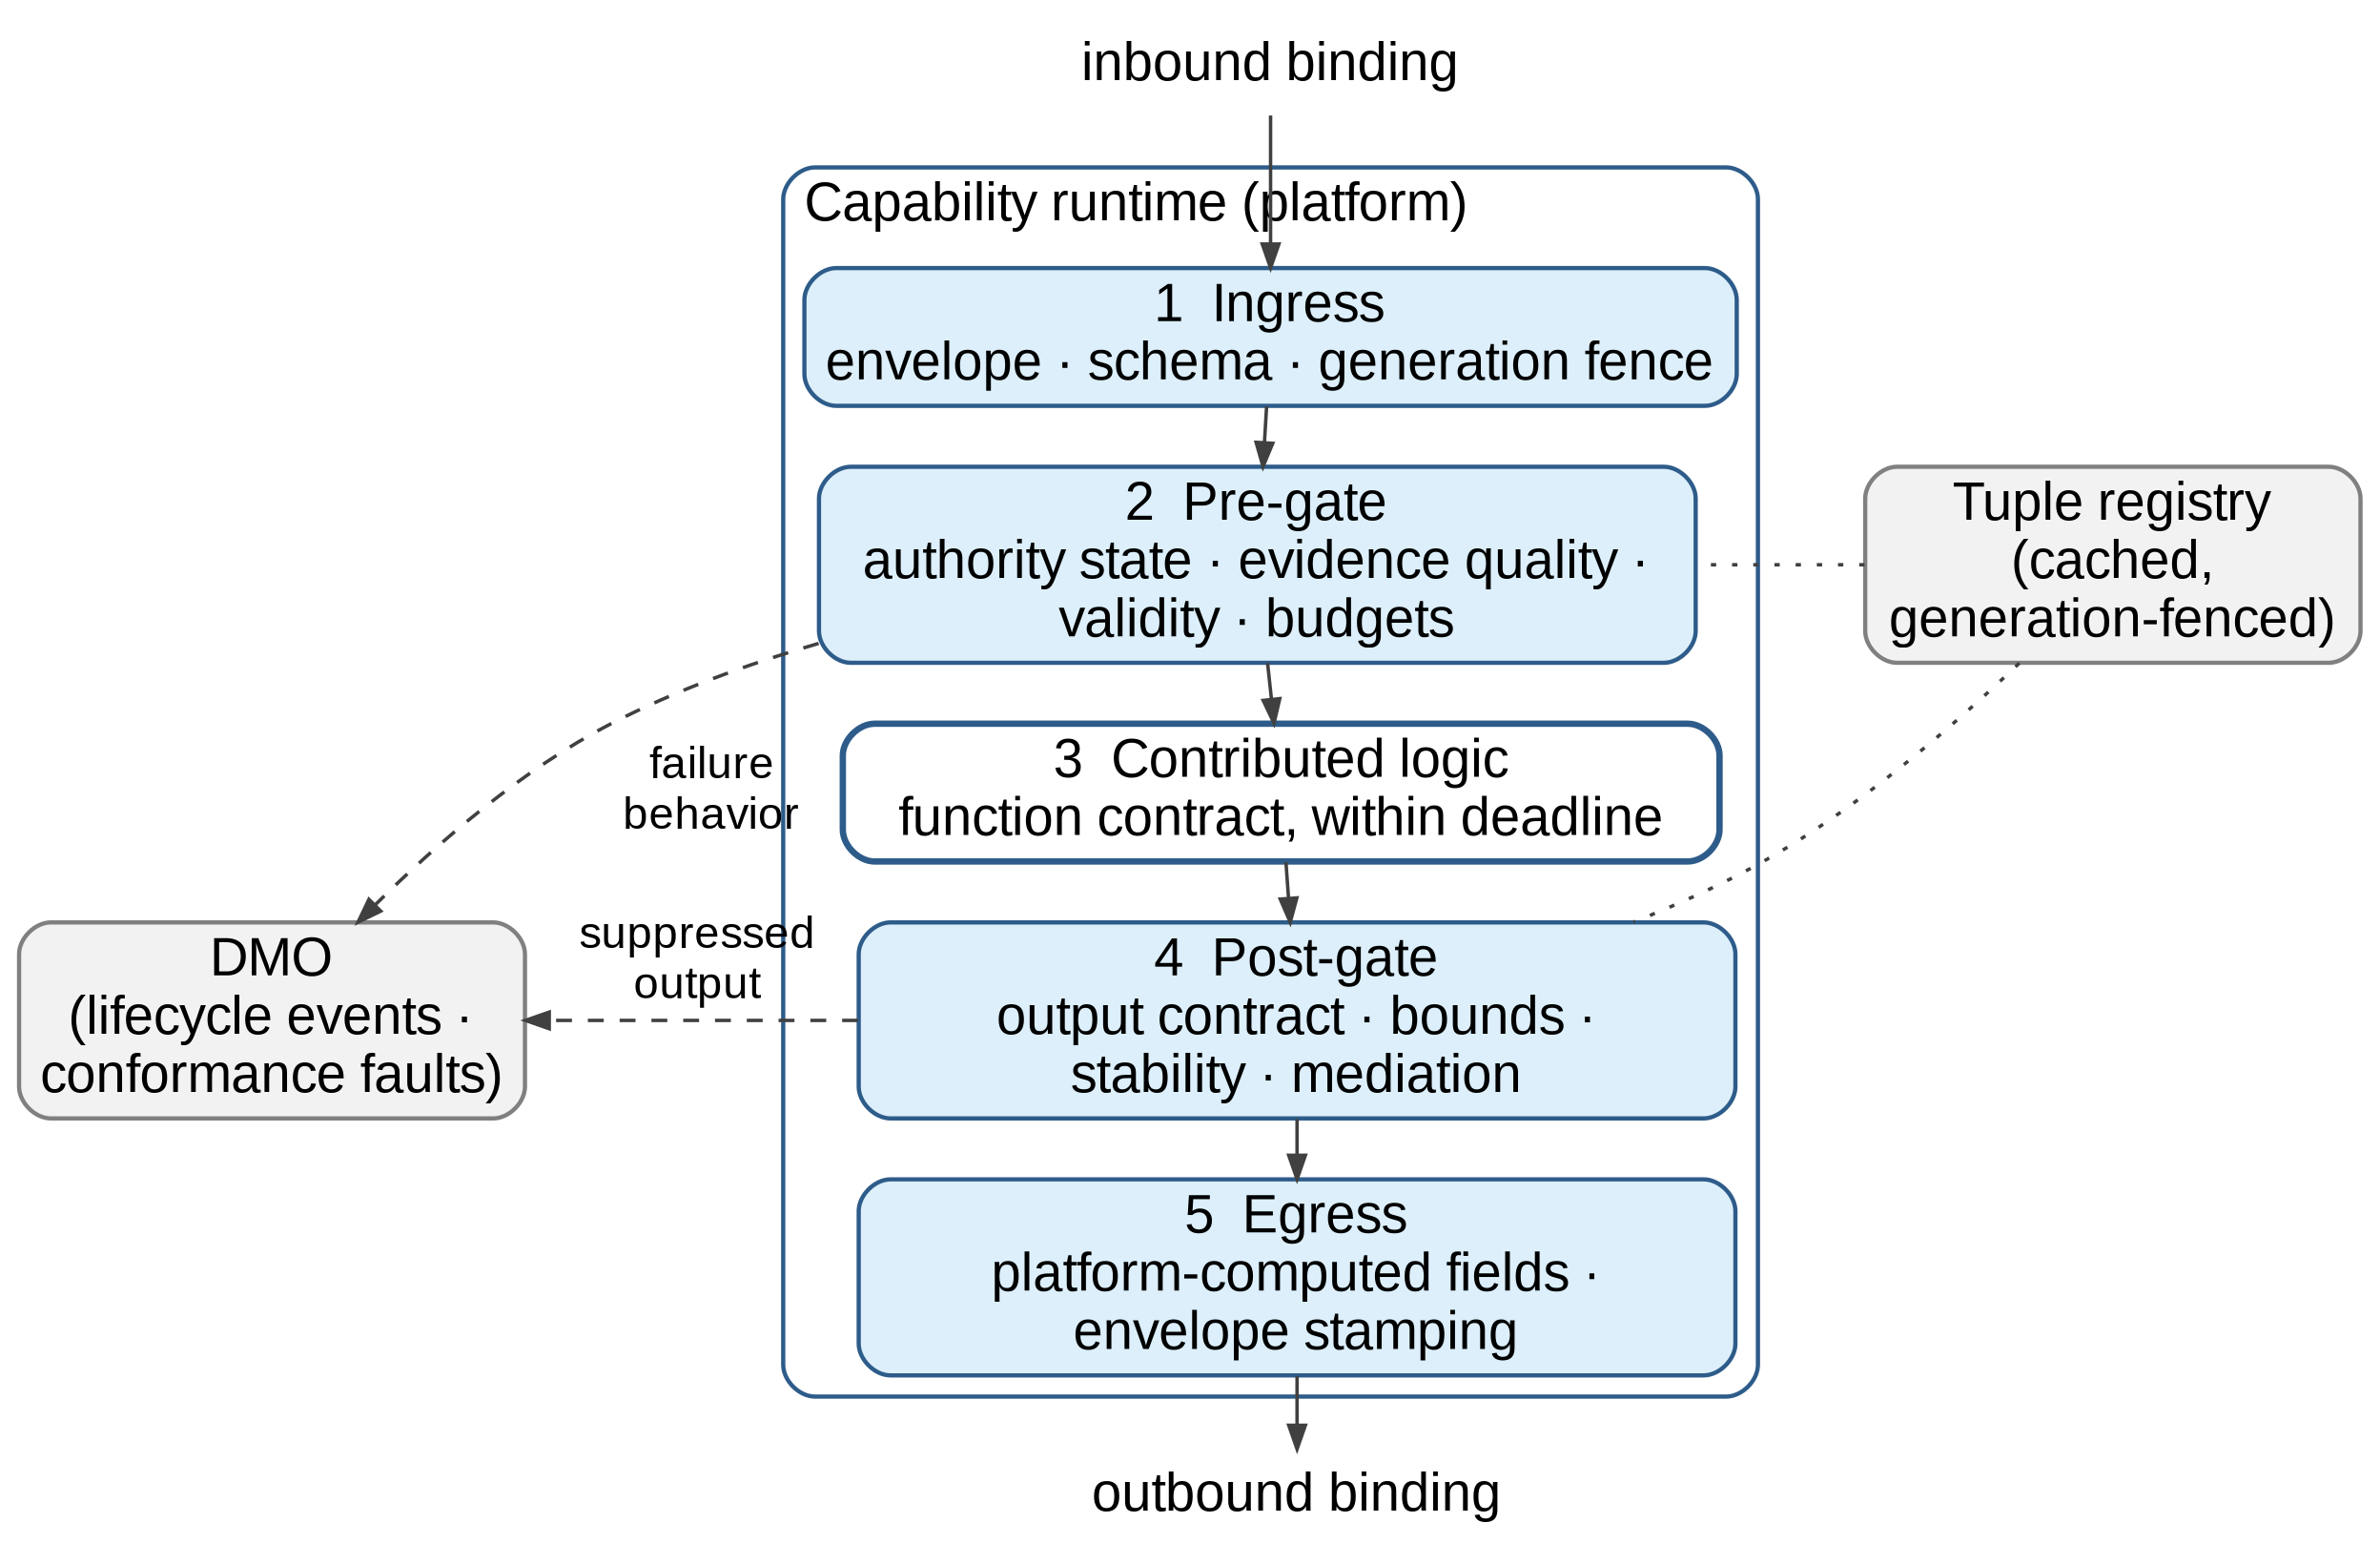
\includegraphics[width=\linewidth,height=0.45\textheight,keepaspectratio]{figures/image4.png}
\captionnum{3-4}
\caption{Execution cycle of a capability}
\label{fig:3-4}
\end{figure}

\hypertarget{function-contracts-and-cycle-order}{%
\subsubsection{Function contracts and cycle order}\label{function-contracts-and-cycle-order}}

The runtime invokes contributed logic through the function contract of
its capability (Table 3-36). A function contract is a logical signature:
it fixes what the logic receives and what it returns, not the
programming language or the transport between runtime and logic.

\begin{wptable}{3-36}

\begin{longtable}[]{@{}
  >{\raggedright\arraybackslash}p{(\columnwidth - 8\tabcolsep) * \real{0.1312}}
  >{\raggedright\arraybackslash}p{(\columnwidth - 8\tabcolsep) * \real{0.1875}}
  >{\raggedright\arraybackslash}p{(\columnwidth - 8\tabcolsep) * \real{0.1312}}
  >{\raggedright\arraybackslash}p{(\columnwidth - 8\tabcolsep) * \real{0.2875}}
  >{\raggedright\arraybackslash}p{(\columnwidth - 8\tabcolsep) * \real{0.2625}}@{}}
\caption{Function contracts of contributed logic}\tabularnewline
\toprule\noalign{}
\begin{minipage}[b]{\linewidth}\raggedright
\textbf{Capability}
\end{minipage} & \begin{minipage}[b]{\linewidth}\raggedright
\textbf{Trigger}
\end{minipage} & \begin{minipage}[b]{\linewidth}\raggedright
\textbf{Function}
\end{minipage} & \begin{minipage}[b]{\linewidth}\raggedright
\textbf{Receives from the runtime}
\end{minipage} & \begin{minipage}[b]{\linewidth}\raggedright
\textbf{Returns}
\end{minipage} \\
\midrule\noalign{}
\endfirsthead
\toprule\noalign{}
\begin{minipage}[b]{\linewidth}\raggedright
\textbf{Capability}
\end{minipage} & \begin{minipage}[b]{\linewidth}\raggedright
\textbf{Trigger}
\end{minipage} & \begin{minipage}[b]{\linewidth}\raggedright
\textbf{Function}
\end{minipage} & \begin{minipage}[b]{\linewidth}\raggedright
\textbf{Receives from the runtime}
\end{minipage} & \begin{minipage}[b]{\linewidth}\raggedright
\textbf{Returns}
\end{minipage} \\
\midrule\noalign{}
\endhead
\bottomrule\noalign{}
\endlastfoot
\textbf{MS} & Periodic, a source event, a schedule, or a request &
collect & Window; scope view of the granted identifiers; declared
sources, read-only & Measurement records: object, metric, value, unit,
event time, sample quality \\
\textbf{AE} & Input arrival with batching window, periodic, a schedule,
or a request & analyze & Consumed observations or data products;
features; context & Insights: insight type, payload, model confidence,
subject scope, validity window \\
\textbf{DE} & Insight arrival, periodic or a schedule; outcomes, verdict
expiries and notifications & decide & Insights, or observations where
the AE is none; objective status; state of the controlled objects; view
of the action space and bounds; live grants & NO\_\allowbreak{}ACTION,
or intent proposals: action type, targets, parameters, validity window,
urgency, decision confidence, rationale \\
\textbf{ACT} & Intent arrival & translate & Mediated intent; state of
the target & Controller commands; the function is deterministic and has
no side effects \\
\end{longtable}

\end{wptable}

The runtime executes the cycle of each capability in the order below. A
step that fails ends the cycle with the consequence stated, and the
failure is reported to the DMO as a lifecycle or conformance event.

The Monitoring System cycle:

\begin{enumerate}
\def\labelenumi{\arabic{enumi}.}
\tightlist
\item
  Supply the window and the scope view, which consists of the concrete
  identifiers of the observation scope granted to the instance.
\item
  Invoke \texttt{collect} within its deadline.
\item
  Discard every record outside the scope view, recording each as a
  conformance fault, and validate metric identifiers and units against
  the observation contract.
\item
  Compute \texttt{scope\_\allowbreak{}coverage} from the scope view and the
  identifiers present, and mark records older than the staleness
  threshold as stale.
\item
  Stamp the envelope and publish, pseudonymizing scope-tag values that
  identify a tenant or a slice where the binding crosses a trust
  boundary.
\end{enumerate}

The Analytics Engine cycle:

\begin{enumerate}
\def\labelenumi{\arabic{enumi}.}
\tightlist
\item
  Assemble the inputs from the observation envelopes or data products
  received for the trigger.
\item
  Compute \texttt{input\_\allowbreak{}quality} from the coverage and timestamps of
  the inputs. Where coverage is below the declared minimum or staleness
  exceeds the declared maximum, execute the declared input behavior
  without invoking the logic.
\item
  Evaluate the validity conditions over the input features and set
  \texttt{validity\_\allowbreak{}state}. Where the state is
  out\_\allowbreak{}of\_\allowbreak{}envelope and the declared behavior
  is insight\_\allowbreak{}unavailable, emit it without invoking the
  logic.
\item
  Invoke \texttt{analyze} within its deadline.
\item
  Check each returned insight against the declared insight types and
  their schemas, and reject any actuation-shaped content.
\item
  Attach \texttt{input\_\allowbreak{}quality}, \texttt{validity\_\allowbreak{}state} and the
  model's provenance, record the inference latency, stamp the envelope
  and publish.
\end{enumerate}

The Decision Engine cycle, executed one cycle at a time per agent
instance:

\begin{enumerate}
\def\labelenumi{\arabic{enumi}.}
\tightlist
\item
  Read the authority state. In
  admitted\_\allowbreak{}not\_\allowbreak{}active,
  monitoring\_\allowbreak{}only and suspended the logic is not invoked;
  in advisory, outputs are routed as recommendations at step 10.
\item
  Check the re-decision budget of each objective. Where it is exhausted,
  raise an objective-unachievable event and do not invoke the logic for
  that objective.
\item
  Evaluate the evidence. Where any consumed input has
  \texttt{degraded\_\allowbreak{}input} set or coverage below the declared minimum,
  execute the declared degraded-evidence behavior; where no usable
  insight is available, execute the declared insight-unavailable
  behavior. In either case the logic is not invoked.
\item
  Invoke \texttt{decide} within its deadline.
\item
  For each proposal whose decision confidence is below the declared
  threshold, execute the declared low-confidence behavior.
\item
  Check each proposal against its contract: the intent schema; the
  action type within the action space and any declared decision-space
  restriction; the parameters within their bounds as narrowed by the
  granted authority and the authority state; the targets within the
  granted control scope; and a complete rationale. A proposal that fails
  is dropped and recorded as a conformance fault.
\item
  Apply the stability controls and rate limit of the action type. A
  proposal that violates them is suppressed and recorded as a
  conformance fault.
\item
  Mediate. A proposal within a live action envelope grant proceeds with
  the grant reference; a proposal for which a held distributed policy
  evaluates as satisfied proceeds with the policy evaluation record;
  every other proposal is submitted to the conflict fabric, and the
  cycle waits for the verdict.
\item
  Apply the verdict. On allow, the proposal proceeds. On modify, the
  proposal is replaced by the returned bounded alternative --- a bounded
  approval being a modify whose alternative is the proposal clamped to
  the returned bounds --- which is re-checked at steps 6 and 7 and
  treated as deny if it fails. The bounds of a verdict apply to the
  proposal submitted and are not retained for later proposals. On defer,
  the proposal is held until its retry-after time, at which the cycle
  resumes from step 1. Deny, and a mediation timeout, execute the
  declared conflict-unresolved behavior.
\item
  Assign the correlation identifier, stamp the envelope with the
  mediation reference and emit the intent to the ACT, or publish it as a
  recommendation in the advisory state.
\end{enumerate}

The Actuator transaction, executed one transaction at a time per target
of an agent instance:

\begin{enumerate}
\def\labelenumi{\arabic{enumi}.}
\tightlist
\item
  Validate the intent's envelope and generation, and the presence and
  liveness of its mediation reference.
\item
  Re-validate the intent against the registry: action space, granted
  control scope, the bounds and expiry of the live grant, and the
  authority state.
\item
  Apply the rate limit and the per-target serialization.
\item
  Evaluate the declared preconditions against the state of the target.
\item
  Invoke \texttt{translate} within its deadline, and check that every
  returned command is a controller operation that the catalog maps to
  the intent's action type.
\item
  Submit the commands through the southbound adapter and wait for at
  most the actuation timeout.
\item
  Classify the response: an explicit refusal is REJECTED; a timeout or a
  loss of transport is UNRESOLVED; an acknowledgement proceeds to
  verification.
\item
  Verify. In-band verification reads back the state through the declared
  method and yields ACKNOWLEDGED\_\allowbreak{}VERIFIED on a match and
  ACKNOWLEDGED\_\allowbreak{}UNVERIFIED otherwise. Deferred verification
  publishes ACKNOWLEDGED\_\allowbreak{}UNVERIFIED marked provisional and
  publishes the final outcome when verification completes or its
  deadline expires.
\item
  Apply the retry matrix and the rollback rules of the declared failure
  policy (Chapter 7).
\item
  Publish the outcome to the DE and to the DMO, and close the
  correlation.
\end{enumerate}

A failure of \texttt{translate}, whether an error or an overrun, ends
the transaction as REJECTED with the reason code
TRANSLATION\_\allowbreak{}FAILED: nothing was submitted, and the state
of the target is known.

\hypertarget{deadlines}{%
\subsubsection{Deadlines}\label{deadlines}}

Each invocation of contributed logic has a deadline. The declared
latency of a capability --- its 99th-percentile latency
\emph{d}\textsubscript{i}, declared in \texttt{operations.latency\_\allowbreak{}p99}
--- is the minimum the capability requires to complete its work, not a
claim on the loop budget.

The time actuation needs is provided for before any slack exists. The
effective loop latency L (Section 3.8.3) contains the declared latency
of the ACT and the mediation and verification terms of its action types
(Table 3-38), so the slack S = B − L of an agent with effective budget B
is what remains once actuation is provided for. The slack is shared
between the capabilities of the loop in proportion to their declared
latencies: the deadline of capability \emph{i} is
\emph{d}\textsubscript{i} + S·\emph{d}\textsubscript{i} /
Σ\emph{d}\textsubscript{j}, so that the deadlines of one loop, together
with its transport, platform overhead, mediation and verification terms,
sum to its budget. No deadline is less than the declared latency of its
capability, and the deadline of the ACT is never reduced to make room
for a capability that precedes it.

The share of slack in a deadline is a tolerance against variation, not
an allowance. The runtime measures each capability against its declared
latency, and a capability whose measured 99th-percentile latency exceeds
it is in breach of its declaration, which Section 3.8.3 resolves by
replacing declared latencies with measured ones and, on a sustained
breach, re-stamping the effective class. An analytics step that runs
slower than planned therefore consumes its own tolerance and never the
time provided for actuation.

Where L exceeds the declared budget, no slack remains and the budget
cannot provide for actuation. The agent is then not admitted at its
declared latency class, and Section 3.8.3 determines whether it is
admitted at a lower class or rejected: an agent is never admitted with a
deadline its actuation cannot meet. For the offline class, the deadline
of each invocation is its declared latency.

An invocation that exceeds its deadline is abandoned by the runtime and
treated as an error of the logic: the MS publishes a gap for the window,
the AE emits insight\_\allowbreak{}unavailable, the DE emits no intent
for the cycle, and the ACT ends the transaction with
TRANSLATION\_\allowbreak{}FAILED.\allowbreak{}

\hypertarget{state-isolation-and-sharing}{%
\subsubsection{State, isolation and sharing}\label{state-isolation-and-sharing}}

Contributed logic may hold state. That state is private to one
capability of one agent instance and is keyed by agentInstanceId. Where
the physical deployment declares a capability stateful, its state is
persisted in the state store provided by the DMO; where it declares the
state retained, the state is restored into each new generation;
otherwise a new generation starts with empty state.

The runtime's own safety state --- re-decision budgets, retry counters,
rate-limit windows, cooldown and reversal timers, and the table of open
correlations --- is held in the state store and survives every restart,
migration and generation change. A new generation inherits it:
restarting an agent never resets a limit the agent has reached.

No state is shared between agent instances. A read-only MS collector may
serve several instances only where the service trees of the instances it
serves declare the collection service
shared\_\allowbreak{}read\_\allowbreak{}only (Table 3-31), and it then
publishes a separately scoped logical stream for each instance.

\hypertarget{time-base}{%
\subsubsection{Time base}\label{time-base}}

Every observation carries the event time at its source and the ingest
time at the MS runtime. Where a source supplies no event time, the
runtime stamps the acquisition time and marks the event time as
acquisition-derived. Timestamps are expressed in RFC 3339 UTC with
microsecond precision. The clocks of the components of one loop shall be
synchronized to within 100 µs in the real-time class, 1 ms in the
near-real-time class and 10 ms in the non-real-time class, so that loop
time, reconfiguration time and staleness are measured on a common time
base.

\hypertarget{latency-classes-and-loop-budgets}{%
\subsection{Latency Classes and Loop Budgets}\label{latency-classes-and-loop-budgets}}

\hypertarget{the-latency-classes}{%
\subsubsection{The latency classes}\label{the-latency-classes}}

The latency classes of the framework are the control-loop timescales of
the Open RAN architecture, adopted unchanged, with an offline class
added for loops that evaluate, predict or plan without acting (Table
3-37). Because the boundaries are those of the standard, a class has the
same meaning in every domain: a transport, orchestration or
non-terrestrial loop is placed by its timescale into the same classes as
a radio loop, and each class corresponds to a tier of deployed
infrastructure with known timing. The real-time class carries the
project's tightest commitments, KPI\#4, KPI\#5 and KPI\#34. Open
implementations of applications hosted at the distributed unit have been
measured closing control loops in under 450 µs on average, so the class
is reachable with a wide margin.

\begin{wptable}{3-37}

\begin{longtable}[]{@{}
  >{\raggedright\arraybackslash}p{(\columnwidth - 6\tabcolsep) * \real{0.1625}}
  >{\raggedright\arraybackslash}p{(\columnwidth - 6\tabcolsep) * \real{0.1562}}
  >{\raggedright\arraybackslash}p{(\columnwidth - 6\tabcolsep) * \real{0.2813}}
  >{\raggedright\arraybackslash}p{(\columnwidth - 6\tabcolsep) * \real{0.4000}}@{}}
\caption{Latency classes}\tabularnewline
\toprule\noalign{}
\begin{minipage}[b]{\linewidth}\raggedright
\textbf{Class}
\end{minipage} & \begin{minipage}[b]{\linewidth}\raggedright
\textbf{Loop budget B}
\end{minipage} & \begin{minipage}[b]{\linewidth}\raggedright
\textbf{Infrastructure tier}
\end{minipage} & \begin{minipage}[b]{\linewidth}\raggedright
\textbf{Conditions and concessions}
\end{minipage} \\
\midrule\noalign{}
\endfirsthead
\toprule\noalign{}
\begin{minipage}[b]{\linewidth}\raggedright
\textbf{Class}
\end{minipage} & \begin{minipage}[b]{\linewidth}\raggedright
\textbf{Loop budget B}
\end{minipage} & \begin{minipage}[b]{\linewidth}\raggedright
\textbf{Infrastructure tier}
\end{minipage} & \begin{minipage}[b]{\linewidth}\raggedright
\textbf{Conditions and concessions}
\end{minipage} \\
\midrule\noalign{}
\endhead
\bottomrule\noalign{}
\endlastfoot
\textbf{real\_\allowbreak{}time} & B \textless{} 10 ms & Applications at
the distributed and central units and at access points, beside the data
they act on & Every flow within a declared latency bound, the bounds
together within B --- LOCAL\_\allowbreak{}RUNTIME presumed, any other
binding class on evidence at admission; every action type on the
envelope or policy path; deferred verification; only local constant-time
guardrails on the per-message path \\
\textbf{near\_\allowbreak{}real\_\allowbreak{}time} & 10 ms ≤ B
\textless{} 1 s & Near-RT RIC applications; transport loops responding
to link events & Action envelopes permitted; verification in band by
default, deferred only for action types whose read-back is slow \\
\textbf{non\_\allowbreak{}real\_\allowbreak{}time} & B ≥ 1 s & Non-RT
RIC and service management and orchestration; IDMO and DMO loops;
planned transport path changes; global agents & Every intent mediated in
band unless covered by a standing grant; every actuation verified in
band \\
\textbf{offline} & No budget & Evaluation, prediction and planning
without acting & Composition classes observation, analytics and
open\_\allowbreak{}loop only; no actuation authority \\
\end{longtable}

\end{wptable}

\hypertarget{loop-time-and-reconfiguration-time}{%
\subsubsection{Loop time and reconfiguration time}\label{loop-time-and-reconfiguration-time}}

\emph{Loop time} is the time from the event time of the earliest
observation that contributed to a decision to the enforcement of the
resulting action at the managed object. \emph{Reconfiguration time} is
the time from the emission of the intent to the same enforcement.
Enforcement is established by verification: its time is the application
time reported in the read-back evidence or, where the managed object
reports none, the time of the controller's acknowledgement of the change
that verification confirmed. A cycle whose outcome is not
ACKNOWLEDGED\_\allowbreak{}VERIFIED has no established enforcement time;
it is excluded from the statistics of loop time and reconfiguration time
and counted separately. KPI\#4 and KPI\#5 are measured as
reconfiguration time, and KPI\#34 as loop time.

\hypertarget{effective-latency-and-class-assignment}{%
\subsubsection{Effective latency and class assignment}\label{effective-latency-and-class-assignment}}

Every agent declares a latency class, a loop budget within the range of
that class, the 99th-percentile latency of each of its capabilities, and
a class policy. At admission the platform computes the effective loop
latency L for the placement proposed by the DMO as the sum of the terms
of Table 3-38. The mediation and verification terms depend on the action
type, so the sum is computed for each action type of the action space
and L is the largest result.

\begin{wptable}{3-38}

\begin{longtable}[]{@{}
  >{\raggedright\arraybackslash}p{(\columnwidth - 2\tabcolsep) * \real{0.1875}}
  >{\raggedright\arraybackslash}p{(\columnwidth - 2\tabcolsep) * \real{0.8125}}@{}}
\caption{Terms of the effective loop latency}\tabularnewline
\toprule\noalign{}
\begin{minipage}[b]{\linewidth}\raggedright
\textbf{Term}
\end{minipage} & \begin{minipage}[b]{\linewidth}\raggedright
\textbf{Value used at admission}
\end{minipage} \\
\midrule\noalign{}
\endfirsthead
\toprule\noalign{}
\begin{minipage}[b]{\linewidth}\raggedright
\textbf{Term}
\end{minipage} & \begin{minipage}[b]{\linewidth}\raggedright
\textbf{Value used at admission}
\end{minipage} \\
\midrule\noalign{}
\endhead
\bottomrule\noalign{}
\endlastfoot
\textbf{Capability latency} & Declared 99th-percentile latency of each
capability (operations.\allowbreak{}latency\_\allowbreak{}p99); for a
delegated capability, the provider\textquotesingle s declared figure. \\
\textbf{Transport} & 99th-percentile latency of each binding between the
capabilities, for its binding class and the placement pair, as published
by the DMO; for LOCAL\_\allowbreak{}RUNTIME within one host, the
runtime\textquotesingle s published figure. \\
\textbf{Platform overhead} & Declared per-cycle overhead of the
capability runtimes, which shall not exceed 5\% of B at the 99th
percentile, nor 0.5 ms in the real-time class. \\
\textbf{Mediation} & Zero for an action type on the envelope or policy
path. Otherwise, the fabric\textquotesingle s measured 99th-percentile
verdict latency for the mediation mode the action requires ---
intra-domain, cross-domain or orchestrator-level --- or, where no
measurement exists, the fabric\textquotesingle s declared timeout for
that mode. \\
\textbf{Verification} & 99th-percentile latency of the declared
verification method for an action type verified in band; zero for
deferred verification. \\
\end{longtable}

\end{wptable}

The platform then assigns the effective class:

\begin{enumerate}
\def\labelenumi{\arabic{enumi}.}
\tightlist
\item
  If L does not exceed the declared budget B, the effective class is the
  declared class and the effective budget is B.
\item
  Otherwise the DMO evaluates the placements available to it that would
  sustain the declared class --- co-locating capabilities, or placing
  inference on more capable compute --- and uses one where it exists,
  and the computation is repeated for that placement.
\item
  If no such placement exists and the class policy is
  accept\_\allowbreak{}lower, the effective class is the class whose
  range contains L, the effective budget is L, and the lowering is
  recorded as a warning in the resolved configuration.
\item
  If no such placement exists and the class policy is
  reject\_\allowbreak{}if\_\allowbreak{}unmet, admission rejects the
  agent.
\end{enumerate}

The effective class, not the declared one, governs composition,
deadlines and the commitments the platform makes. At runtime, measured
latencies replace declared ones, and a sustained breach re-stamps the
effective class downward (Chapter 12).

An agent holds the real-time class only if every flow of its loop meets
a latency bound within the loop budget, every action type of its action
space is on the envelope or policy path, and the verification of every
action type is deferred with a declared deadline. A
LOCAL\_\allowbreak{}RUNTIME binding is presumed to meet the bound and is
declared without further evidence. Any other binding class is admissible
on a flow of a real-time loop where the descriptor declares the bound
the flow achieves and admission is supplied with evidence for it --- a
measurement on the proposed placement, or a commitment of the transport
that carries the flow --- sufficient for the sum of the bounds of the
loop's flows to lie within the loop budget. The class is a property of
the latency the loop achieves, not of the placement by which it achieves
it; a flow admitted on declared evidence is subject to the same runtime
re-stamping as any other. An intent of a real-time agent that falls
outside its live action envelope remains permitted: it is submitted for
mediation, and its cycle is recorded as outside the class commitment.

\hypertarget{non-terrestrial-segments}{%
\subsubsection{Non-terrestrial segments}\label{non-terrestrial-segments}}

Propagation over a non-terrestrial segment is a property of distance and
cannot be reduced by resources. A loop whose path crosses a
non-terrestrial segment shall not hold the real-time class. The
project's relaxation of its control-loop commitment by an order of
magnitude for non-terrestrial deployments (KPI\#34) corresponds to a
loop budget of 100 ms, which lies in the near-real-time class. Because
the transport terms of the effective latency are computed from the
actual placement, a capability placed across such a segment from the
rest of its loop is visible at admission and cannot take part in a loop
faster than the segment allows.

\hypertarget{authority-and-bounds}{%
\subsection{Authority and Bounds}\label{authority-and-bounds}}

\hypertarget{the-bound-stack}{%
\subsubsection{The bound stack}\label{the-bound-stack}}

An action of an agent is permitted if, and only if, it lies within every
one of the five bounds of Table 3-39. Each bound is set by a different
party and held by the platform, never by the agent. A bound may narrow
what the bounds before it permit; none may widen it. In particular,
neither a modify verdict nor an action envelope can authorize an action
outside the declared contract or the granted authority, and no authority
state restores scope that was withheld at admission.

\begin{wptable}{3-39}

\begin{longtable}[]{@{}
  >{\raggedright\arraybackslash}p{(\columnwidth - 8\tabcolsep) * \real{0.1750}}
  >{\raggedright\arraybackslash}p{(\columnwidth - 8\tabcolsep) * \real{0.3000}}
  >{\raggedright\arraybackslash}p{(\columnwidth - 8\tabcolsep) * \real{0.1813}}
  >{\raggedright\arraybackslash}p{(\columnwidth - 8\tabcolsep) * \real{0.1438}}
  >{\raggedright\arraybackslash}p{(\columnwidth - 8\tabcolsep) * \real{0.2000}}@{}}
\caption{The bound stack}\tabularnewline
\toprule\noalign{}
\begin{minipage}[b]{\linewidth}\raggedright
\textbf{Bound}
\end{minipage} & \begin{minipage}[b]{\linewidth}\raggedright
\textbf{Content}
\end{minipage} & \begin{minipage}[b]{\linewidth}\raggedright
\textbf{Set by}
\end{minipage} & \begin{minipage}[b]{\linewidth}\raggedright
\textbf{Held in}
\end{minipage} & \begin{minipage}[b]{\linewidth}\raggedright
\textbf{Checked at}
\end{minipage} \\
\midrule\noalign{}
\endfirsthead
\toprule\noalign{}
\begin{minipage}[b]{\linewidth}\raggedright
\textbf{Bound}
\end{minipage} & \begin{minipage}[b]{\linewidth}\raggedright
\textbf{Content}
\end{minipage} & \begin{minipage}[b]{\linewidth}\raggedright
\textbf{Set by}
\end{minipage} & \begin{minipage}[b]{\linewidth}\raggedright
\textbf{Held in}
\end{minipage} & \begin{minipage}[b]{\linewidth}\raggedright
\textbf{Checked at}
\end{minipage} \\
\midrule\noalign{}
\endhead
\bottomrule\noalign{}
\endlastfoot
\textbf{1. Declared contract} & Action space with bounds, rate limits
and stability controls; observation and control scope & Contributor, in
the descriptor & Registry, from admission & Admission; DE post-gate; ACT
last-mile check \\
\textbf{2. Granted authority} & Granted control scope, narrowed bounds,
priority band, authority ceiling; for a delegation, the authority
envelope & IDMO and DMO, at admission or in the delegation & Registry &
Admission; DE post-gate; ACT last-mile check \\
\textbf{3. Authority state} & One of the seven states of Table 3-12 &
DMO or IDMO: activation gate, evaluation, lifecycle & Registry & DE
pre-gate, every cycle; ACT last-mile check \\
\textbf{4. Mediation} & Verdict, action envelope grant or distributed
policy & Conflict fabric & Registry for grants; message for verdict
references & DE post-gate; ACT last-mile check against the live grant \\
\textbf{5. Class and KPI bounds} & Effective latency class and budget;
bounds derived from project KPIs & Admission, from the class definitions
and project KPIs & Registry & Admission; runtime measurement \\
\end{longtable}

\end{wptable}

\hypertarget{envelopes-of-authority}{%
\subsubsection{Envelopes of authority}\label{envelopes-of-authority}}

Three mechanisms pre-authorize action so that it can proceed without a
round trip, and all three have the same shape: a bounded region of
permitted action, with a validity window, inside which action proceeds
and outside which approval is required. The \emph{action envelope} is
granted by the conflict fabric over a region of an agent's action space,
and is what makes the real-time class compatible with mediation. The
\emph{authority envelope} is granted by the IDMO to a DMO in a
delegation, and is what makes hierarchy compatible with local latency.
The \emph{distributed policy} is granted by the fabric on request, and
lets an agent establish conflict-freedom locally where the region cannot
be enumerated in advance. In each case authority originates with the
granting party, and the agent acts only within authority already
granted; an agent never authorizes itself.

A grant is void when its validity expires, when the granting party
withdraws it, and when the agent's underlying domain service is migrated
or terminated by orchestration. Voiding takes effect at the next
last-mile check of the ACT, which checks every command against the live
grant rather than a cached copy.

\hypertarget{bounds-derived-from-kpis}{%
\subsubsection{Bounds derived from KPIs}\label{bounds-derived-from-kpis}}

The bounds of the latency classes and of the platform's own overhead are
derived from the project KPIs: the real-time class from KPI\#4, KPI\#5
and KPI\#34, and the per-cycle overhead of the guardrails --- at most
5\% of the loop budget at the 99th percentile, and 0.5 ms in the
real-time class --- from the same commitments. An agent whose
declaration cannot meet the bounds of the class it requests is assigned
a class it can sustain, or rejected, at admission (Section 3.8.3); an
agent whose measured behavior leaves those bounds during operation is
re-classed or demoted. Chapter 12 derives the full set of bounds from
the project KPIs and states for each whether an agent outside it is
re-classed, demoted or rejected.

\hypertarget{coexistence-with-conventionally-managed-services}{%
\subsection{Coexistence with Conventionally Managed Services}\label{coexistence-with-conventionally-managed-services}}

The architecture accommodates several ways of realizing a managed
service, and services defined conventionally, without tuples, coexist
with agent-managed services in the same deployment. The following rules
govern the boundary between them.

\begin{itemize}
\tightlist
\item
  A domain in which no agent is instantiated is managed without one. No
  tuple artifact is instantiated there, and nothing in this framework
  applies to the services in that domain.
\item
  Agent instantiation is independent of service orchestration, so one
  end-to-end service may span agent-managed domains and conventionally
  managed ones.
\item
  An automated control function outside the framework, such as a legacy
  optimization function or a loop internal to a controller, that acts on
  control parameters in a domain where agents hold control scope shall
  either take part in conflict mediation, submitting its actions as an
  agent does, or have the control parameters it acts on reserved. A
  reserved parameter is registered with the conflict fabric as held by
  an external controller and shall not be granted to the control scope
  of any agent. The DMO applies this rule when it grants control scope.
\item
  A manual intervention by an operator on control parameters within an
  agent's granted control scope takes precedence over the agent. The DMO
  withdraws those parameters from the agent's granted control scope from
  the moment of the intervention and holds them withdrawn until control
  over them is explicitly returned. The hold does not expire, and no
  elapsed interval, restored objective or later agent proposal ends it:
  a human decision stands until a human reverses it. A held parameter is
  registered with the conflict fabric as held, and the DMO raises a
  standing assurance signal, from the moment of the hold until its
  return, naming the parameter, the agent whose scope it left and the
  time the hold began, so that a hold left in place is visible to
  operations rather than silent. The agent continues to operate on the
  remainder of its granted control scope where its descriptor declares
  objectives that remain achievable without the held parameter; where it
  does not, the agent enters the degraded operation its failure policy
  declares, and the cause recorded is the hold and not a fault of the
  agent. Any action envelope held against a withdrawn parameter is
  voided. A recommendation of an open-loop agent that an operator
  applies is such an intervention.
\item
  A lifecycle operation of the orchestration layer on an agent's
  underlying domain service --- migration, scaling or termination --- is
  a lifecycle event for the agent: the generation is incremented,
  decision authority is suspended from the moment the operation begins,
  and any action envelope held against the affected scope is voided
  (Chapter 9).
\item
  Observation confers no control. An agent may observe conventionally
  managed resources within its observation scope, and its control scope
  contains only what admission grants.
\end{itemize}

\hypertarget{requirements}{%
\subsection{Requirements}\label{requirements}}

The requirements of the agentic framework that are not specific to one
capability are listed in the tables below.

\begin{requirement}{Req-T23-FW-01}{MUST}{Tuple composition}
\reqfield{Description / rationale}{%
Every agent shall be composed of the four capabilities MS, AE, DE and
ACT, each declared in its descriptor in exactly one capability mode:
full, partial, delegated or none. The platform shall derive the
agent\textquotesingle s composition class from the declared modes, and
the class shall bound the highest authority state the agent can hold. A
descriptor whose modes fit no composition class shall be invalid.}
\reqfield{Dependency}{%
None}
\reqfield{Traceability (Forward)}{%
\begin{itemize}
\item
  Checked by the validity rules before admission.
\item
  Composition class recorded in the registry and reported in assurance.
\end{itemize}}
\reqfield{UNITY-6G components}{%
\begin{itemize}
\item
  Tuple descriptor
\item
  Tuple registry and admission (IDMO/DMO)
\end{itemize}}
\reqfield{Linked KPIs}{%
\begin{itemize}
\item
  KPI\#1: Deliver four distributed management entities (MS, AE, DE and
  ACT) deployable in each heterogeneous domain.
\item
  KPI\#26: Increase the ratio of service management and LCM tasks
  resolved by local AE/DE components.
\end{itemize}}
\end{requirement}

\begin{requirement}{Req-T23-FW-02}{MUST}{Typed capability outputs}
\reqfield{Description / rationale}{%
Each capability shall produce only its own semantic object: observations
from the MS, insights from the AE, intents from the DE and outcomes from
the ACT. A contract whose schema carries content of another
capability\textquotesingle s output --- model outputs in an observation,
actuation-shaped fields in an insight, controller-native commands in an
intent --- shall be rejected, and an object carrying such content shall
be rejected at the binding boundary.}
\reqfield{Dependency}{%
Req-T23-FW-01}
\reqfield{Traceability (Forward)}{%
\begin{itemize}
\item
  Checked by the validity rules against the declared schemas.
\item
  Enforced at every binding boundary by the capability runtimes.
\end{itemize}}
\reqfield{UNITY-6G components}{%
\begin{itemize}
\item
  Capability runtimes
\item
  Tuple descriptor
\end{itemize}}
\reqfield{Linked KPIs}{%
\begin{itemize}
\item
  KPI\#1: Deliver four distributed management entities (MS, AE, DE and
  ACT) deployable in each heterogeneous domain.
\item
  KPI\#36: Guarantee 99.99999\% service availability and reliability
  based on effective monitoring and LCM.
\end{itemize}}
\end{requirement}

\begin{requirement}{Req-T23-FW-03}{MUST}{Capability mode obligations}
\reqfield{Description / rationale}{%
A partial capability shall enumerate its subset. A delegated capability
shall name its provider, the provider\textquotesingle s interface, a
pinned interface profile, a range of accepted provider versions and its
SLA assumptions, and admission shall verify that the
provider\textquotesingle s scope covers the consumer\textquotesingle s
and that the provider\textquotesingle s declared latency and freshness
meet those assumptions. MS and ACT delegations shall remain within the
domain; an AE delegation may cross domains as a data product or an
exposed contract; a DE delegation may cross domains only to the
agent\textquotesingle s own global agent.}
\reqfield{Dependency}{%
Req-T23-FW-01}
\reqfield{Traceability (Forward)}{%
\begin{itemize}
\item
  Checked by the validity rules and at admission.
\item
  Binding fault raised at runtime when a provider leaves the pinned
  range.
\end{itemize}}
\reqfield{UNITY-6G components}{%
\begin{itemize}
\item
  Tuple descriptor
\item
  Admission (IDMO/DMO)
\item
  Provider agents and reused capabilities
\end{itemize}}
\reqfield{Linked KPIs}{%
\begin{itemize}
\item
  KPI\#1: Deliver four distributed management entities (MS, AE, DE and
  ACT) deployable in each heterogeneous domain.
\item
  KPI\#36: Guarantee 99.99999\% service availability and reliability
  based on effective monitoring and LCM.
\end{itemize}}
\end{requirement}

\begin{requirement}{Req-T23-FW-04}{MUST}{The descriptor as the single contract}
\reqfield{Description / rationale}{%
An agent\textquotesingle s scope, objectives, action space, failure
behavior, latency class and permitted bindings shall be read only from
its admitted descriptor, from the values bound at its instantiation and
from the delegation it realizes, where it realizes one. No value
reported by an agent at runtime shall extend them, and a
platform-computed field shall never be accepted from contributed logic.}
\reqfield{Dependency}{%
None}
\reqfield{Traceability (Forward)}{%
\begin{itemize}
\item
  Enforced by admission and by the capability runtimes.
\end{itemize}}
\reqfield{UNITY-6G components}{%
\begin{itemize}
\item
  Tuple registry
\item
  Capability runtimes
\end{itemize}}
\reqfield{Linked KPIs}{%
\begin{itemize}
\item
  KPI\#33: Support more tenants via distributed AI \& DLT.
\item
  KPI\#36: Guarantee 99.99999\% service availability and reliability
  based on effective monitoring and LCM.
\end{itemize}}
\end{requirement}

\begin{requirement}{Req-T23-FW-05}{MUST}{Descriptor structure}
\reqfield{Description / rationale}{%
A descriptor shall contain the sections of Table 3-13 required for its
composition class, and no section marked absent for that class, and
shall conform to the schema version it declares. Payload schemas shall
be JSON Schema 2020-12 documents referenced by identifier and version,
and predicates shall be structured conditions of the form defined in
Table 3-3, evaluable without an expression interpreter.}
\reqfield{Dependency}{%
Req-T23-FW-01}
\reqfield{Traceability (Forward)}{%
\begin{itemize}
\item
  Validated against the JSON Schema rendering of the descriptor (Annex
  A).
\end{itemize}}
\reqfield{UNITY-6G components}{%
\begin{itemize}
\item
  Tuple descriptor
\item
  Schema registry
\end{itemize}}
\reqfield{Linked KPIs}{%
\begin{itemize}
\item
  KPI\#1: Deliver four distributed management entities (MS, AE, DE and
  ACT) deployable in each heterogeneous domain.
\item
  KPI\#46: Availability of four open-source frameworks and their
  corresponding API specifications for the UNITY-6G PoCs.
\end{itemize}}
\end{requirement}

\begin{requirement}{Req-T23-FW-06}{MUST}{Validity before admission}
\reqfield{Description / rationale}{%
A descriptor shall satisfy every validity rule of Table 3-30 before it
is submitted to admission. A failure shall be reported with the
identifier of every rule violated, and a descriptor that fails any rule
shall not be admitted.}
\reqfield{Dependency}{%
Req-T23-FW-05}
\reqfield{Traceability (Forward)}{%
\begin{itemize}
\item
  Checked by a validator that operates on the descriptor, its schemas
  and the catalog alone.
\end{itemize}}
\reqfield{UNITY-6G components}{%
\begin{itemize}
\item
  Descriptor validator
\item
  Type catalog
\end{itemize}}
\reqfield{Linked KPIs}{%
\begin{itemize}
\item
  KPI\#6: Decrease service creation and termination time.
\item
  KPI\#41: Reduction of 70\% of deployment time of AI-based
  resource/energy management algorithms.
\end{itemize}}
\end{requirement}

\begin{requirement}{Req-T23-FW-07}{MUST}{Versioning and immutability}
\reqfield{Description / rationale}{%
A descriptor shall be identified by its descriptor\_\allowbreak{}id and
a semantic version. An admitted version shall be immutable: any change
to its content, artifacts, models or parameters shall produce a new
version, admitted as a new descriptor. The registry shall record the
content hash of every admitted version, and every instance shall
reference exactly one version.}
\reqfield{Dependency}{%
Req-T23-FW-08}
\reqfield{Traceability (Forward)}{%
\begin{itemize}
\item
  Checked at admission against the registry.
\end{itemize}}
\reqfield{UNITY-6G components}{%
\begin{itemize}
\item
  Tuple registry
\item
  Type catalog
\end{itemize}}
\reqfield{Linked KPIs}{%
\begin{itemize}
\item
  KPI\#33: Support more tenants via distributed AI \& DLT.
\item
  KPI\#37: Guarantee 99.99999\% service continuity through AI-driven
  proactive management of cloud-native services.
\end{itemize}}
\end{requirement}

\begin{requirement}{Req-T23-FW-08}{MUST}{Integrity}
\reqfield{Description / rationale}{%
A descriptor shall carry a content hash over its canonical form (RFC
8785) and the signature of its publisher; every artifact shall be
referenced by digest with a software bill of materials that pins each
software dependency, and every platform service the agent requires shall
be declared with a minimum version. A descriptor whose hash or signature
does not verify against the publisher\textquotesingle s key in its trust
domain shall be rejected before any other check.}
\reqfield{Dependency}{%
None}
\reqfield{Traceability (Forward)}{%
\begin{itemize}
\item
  Verified first at admission.
\item
  Attestations checked where the trust domain requires them.
\end{itemize}}
\reqfield{UNITY-6G components}{%
\begin{itemize}
\item
  Tuple registry
\item
  Trust layer (T2.4)
\end{itemize}}
\reqfield{Linked KPIs}{%
\begin{itemize}
\item
  KPI\#33: Support more tenants via distributed AI \& DLT.
\end{itemize}}
\end{requirement}

\begin{requirement}{Req-T23-FW-09}{MUST}{Bounded extension}
\reqfield{Description / rationale}{%
Extension fields shall be named
x-\textless publisher\textgreater-\textless name\textgreater{} and shall
appear only at the top level of the descriptor, within the capability
sections of functions and within model\_\allowbreak{}hooks; they shall
not appear in scope, action\_\allowbreak{}space, policies,
failure\_\allowbreak{}policy, interfaces,
physical\_\allowbreak{}deployment, ownership or integrity. A descriptor
containing any extension field or extension type shall be of extension
conformance and shall enter at the advisory authority state.}
\reqfield{Dependency}{%
Req-T23-FW-05}
\reqfield{Traceability (Forward)}{%
\begin{itemize}
\item
  Checked by the validity rules.
\item
  Conformance class recorded in the registry.
\end{itemize}}
\reqfield{UNITY-6G components}{%
\begin{itemize}
\item
  Tuple descriptor
\item
  Admission (IDMO/DMO)
\end{itemize}}
\reqfield{Linked KPIs}{%
\begin{itemize}
\item
  KPI\#33: Support more tenants via distributed AI \& DLT.
\item
  KPI\#41: Reduction of 70\% of deployment time of AI-based
  resource/energy management algorithms.
\end{itemize}}
\end{requirement}

\begin{requirement}{Req-T23-FW-10}{MUST}{Descriptor levels}
\reqfield{Description / rationale}{%
A local agent shall be described by a LocalAINativeAgent descriptor
owned by a DMO, and a global agent by a GlobalAINativeAgent descriptor
owned by the IDMO. The IDMO shall address a domain on behalf of a global
agent only through DomainAgentDelegation documents. Neither a global
descriptor nor a delegation shall contain domain-internal placement,
deployment or controller mapping.}
\reqfield{Dependency}{%
Req-T23-FW-05}
\reqfield{Traceability (Forward)}{%
\begin{itemize}
\item
  Checked by the validity rules and at admission.
\end{itemize}}
\reqfield{UNITY-6G components}{%
\begin{itemize}
\item
  IDMO
\item
  DMO
\item
  Tuple descriptor
\end{itemize}}
\reqfield{Linked KPIs}{%
\begin{itemize}
\item
  KPI\#1: Deliver four distributed management entities (MS, AE, DE and
  ACT) deployable in each heterogeneous domain.
\item
  KPI\#18: Reduction in the deployment time of heterogeneous domain
  services.
\item
  KPI\#26: Increase the ratio of service management and LCM tasks
  resolved by local AE/DE components.
\end{itemize}}
\end{requirement}

\begin{requirement}{Req-T23-FW-11}{MUST}{Agent service tree}
\reqfield{Description / rationale}{%
An agent descriptor shall declare the service tree of its tuples,
stating for each tuple the services it requires in order to perform its
capability and the bindings that interconnect the tuples into a closed
loop. A GlobalAINativeAgent descriptor shall be issued to the IDMO and a
LocalAINativeAgent descriptor to the DMO of its domain, and the
receiving orchestrator shall instantiate the declared services and bind
them before the agent is activated. A resource-facing service shall
carry no agent content.}
\reqfield{Dependency}{%
Req-T23-FW-04}
\reqfield{Traceability (Forward)}{%
\begin{itemize}
\item
  Checked at admission of the descriptor and at instantiation.
\end{itemize}}
\reqfield{UNITY-6G components}{%
\begin{itemize}
\item
  IDMO
\item
  DMO
\end{itemize}}
\reqfield{Linked KPIs}{%
\begin{itemize}
\item
  KPI\#1: Deliver four distributed management entities (MS, AE, DE and
  ACT) deployable in each heterogeneous domain.
\item
  KPI\#6: Decrease service creation and termination time.
\item
  KPI\#18: Reduction in the deployment time of heterogeneous domain
  services.
\end{itemize}}
\end{requirement}

\begin{requirement}{Req-T23-FW-12}{MUST}{Isolation of instances}
\reqfield{Description / rationale}{%
Every agent instance shall be isolated by the triple
descriptor\_\allowbreak{}id, assignedDomainId and agentInstanceId, with
its own policy state, model state, decision history, action correlation,
evaluation windows and lifecycle. A monitoring collector shall be shared
between instances only where the service trees of the instances it
serves declare the collection service
shared\_\allowbreak{}read\_\allowbreak{}only, and shall then publish a
separately scoped logical stream for each instance.}
\reqfield{Dependency}{%
Req-T23-FW-11}
\reqfield{Traceability (Forward)}{%
\begin{itemize}
\item
  Enforced by the DMO at realization and by the capability runtimes.
\end{itemize}}
\reqfield{UNITY-6G components}{%
\begin{itemize}
\item
  DMO
\item
  Capability runtimes
\item
  State store
\end{itemize}}
\reqfield{Linked KPIs}{%
\begin{itemize}
\item
  KPI\#33: Support more tenants via distributed AI \& DLT.
\item
  KPI\#36: Guarantee 99.99999\% service availability and reliability
  based on effective monitoring and LCM.
\end{itemize}}
\end{requirement}

\begin{requirement}{Req-T23-FW-13}{MUST}{Generation fencing}
\reqfield{Description / rationale}{%
The owning DMO or IDMO shall assign each agent instance a generation,
incremented at every placement, restart, migration, model update and
binding change, and at migration or termination of the underlying domain
service. Every message shall carry its producer\textquotesingle s
generation. A receiver shall discard a message of an older generation
than its binding record, and shall refresh the record from the registry
before accepting a message of a newer one.}
\reqfield{Dependency}{%
Req-T23-FW-12}
\reqfield{Traceability (Forward)}{%
\begin{itemize}
\item
  Enforced by every receiving runtime.
\end{itemize}}
\reqfield{UNITY-6G components}{%
\begin{itemize}
\item
  DMO / IDMO
\item
  Capability runtimes
\end{itemize}}
\reqfield{Linked KPIs}{%
\begin{itemize}
\item
  KPI\#36: Guarantee 99.99999\% service availability and reliability
  based on effective monitoring and LCM.
\item
  KPI\#37: Guarantee 99.99999\% service continuity through AI-driven
  proactive management of cloud-native services.
\end{itemize}}
\end{requirement}

\begin{requirement}{Req-T23-FW-14}{MUST}{Hosted contributed logic}
\reqfield{Description / rationale}{%
Contributed logic shall execute within the capability runtime of its
capability. All binding exchanges, platform-computed fields, gates,
counters, rate limits and southbound submissions shall be performed by
the runtime. Contributed logic shall open no binding, bus session or
controller session; its only input and output beyond the runtime shall
be read-only access by an MS to its declared sources, and the declared
read-only tools of a generative DE.}
\reqfield{Dependency}{%
None}
\reqfield{Traceability (Forward)}{%
\begin{itemize}
\item
  Verified at the activation gate.
\item
  Exercised in the WP6 proofs of concept.
\end{itemize}}
\reqfield{UNITY-6G components}{%
\begin{itemize}
\item
  Capability runtimes
\item
  DMO
\end{itemize}}
\reqfield{Linked KPIs}{%
\begin{itemize}
\item
  KPI\#1: Deliver four distributed management entities (MS, AE, DE and
  ACT) deployable in each heterogeneous domain.
\item
  KPI\#36: Guarantee 99.99999\% service availability and reliability
  based on effective monitoring and LCM.
\item
  KPI\#46: Availability of four open-source frameworks and their
  corresponding API specifications for the UNITY-6G PoCs.
\end{itemize}}
\end{requirement}

\begin{requirement}{Req-T23-FW-15}{MUST}{Function contracts and deadlines}
\reqfield{Description / rationale}{%
The runtime shall invoke contributed logic only through the function
contract of its capability (Table 3-36), in the cycle order of Section
3.7.2 and within the deadline of Section 3.7.3. An overrun or an error
shall be treated as the capability\textquotesingle s declared
unavailability: a gap for the MS, insight\_\allowbreak{}unavailable for
the AE, no intent for the DE, and TRANSLATION\_\allowbreak{}FAILED for
the ACT.}
\reqfield{Dependency}{%
Req-T23-FW-14}
\reqfield{Traceability (Forward)}{%
\begin{itemize}
\item
  Enforced by the capability runtimes.
\end{itemize}}
\reqfield{UNITY-6G components}{%
\begin{itemize}
\item
  Capability runtimes
\end{itemize}}
\reqfield{Linked KPIs}{%
\begin{itemize}
\item
  KPI\#4: Real-time reconfiguration of IEEE 802.11 network domain in
  range smaller than 10 ms from taking the decision.
\item
  KPI\#5: Real-time reconfiguration of cellular network domain in the
  range smaller than 10 ms from taking the decision.
\item
  KPI\#34: Reduce Open RAN real-time control loops time scales below 10
  ms and 10x in NTN for real-time 6G.
\end{itemize}}
\end{requirement}

\begin{requirement}{Req-T23-FW-16}{MUST}{Serial decision and actuation}
\reqfield{Description / rationale}{%
The decision cycles of one agent instance shall be serial. The actuation
transactions of one agent instance on one target shall be serial;
transactions on distinct targets may run concurrently up to the declared
maximum concurrency.}
\reqfield{Dependency}{%
Req-T23-FW-15}
\reqfield{Traceability (Forward)}{%
\begin{itemize}
\item
  Enforced by the DE and ACT runtimes.
\end{itemize}}
\reqfield{UNITY-6G components}{%
\begin{itemize}
\item
  Capability runtimes
\end{itemize}}
\reqfield{Linked KPIs}{%
\begin{itemize}
\item
  KPI\#21: Reduce the performance penalty due to conflicts by 20\% by
  means of DLT, hierarchical algorithms and policy-based conflict
  resolution schemes.
\item
  KPI\#36: Guarantee 99.99999\% service availability and reliability
  based on effective monitoring and LCM.
\end{itemize}}
\end{requirement}

\begin{requirement}{Req-T23-FW-17}{MUST}{Deterministic translation}
\reqfield{Description / rationale}{%
The ACT\textquotesingle s translation of intent into controller commands
shall be deterministic and free of side effects, and every command it
returns shall be a controller operation that the catalog maps to the
intent\textquotesingle s action type. Learned, generative and
simulation-based techniques shall not be admitted as translation logic.}
\reqfield{Dependency}{%
Req-T23-FW-18}
\reqfield{Traceability (Forward)}{%
\begin{itemize}
\item
  Checked at admission from the declared technique.
\item
  Command mapping checked by the ACT runtime in every transaction.
\end{itemize}}
\reqfield{UNITY-6G components}{%
\begin{itemize}
\item
  ACT runtime
\item
  Type catalog
\end{itemize}}
\reqfield{Linked KPIs}{%
\begin{itemize}
\item
  KPI\#36: Guarantee 99.99999\% service availability and reliability
  based on effective monitoring and LCM.
\item
  KPI\#42: DT-validated AI algorithms that do not break the
  time-sensitive operation when deployed in 99\% of the outputs.
\end{itemize}}
\end{requirement}

\begin{requirement}{Req-T23-FW-18}{MUST}{Technique admissibility}
\reqfield{Description / rationale}{%
Contributed logic shall declare its technique class per capability and
shall be admitted only under the conditions of Table 3-11. A generative
DE shall hold no tool that changes network state. Adaptation that
changes model weights shall produce a new model identity and take effect
only through a generation-controlled update; adaptation by accumulated
context shall declare its retained-context bound and reset condition.}
\reqfield{Dependency}{%
None}
\reqfield{Traceability (Forward)}{%
\begin{itemize}
\item
  Checked at admission.
\item
  Model identity checked at the activation gate.
\end{itemize}}
\reqfield{UNITY-6G components}{%
\begin{itemize}
\item
  Admission (IDMO/DMO)
\item
  AI/ML domain
\end{itemize}}
\reqfield{Linked KPIs}{%
\begin{itemize}
\item
  KPI\#41: Reduction of 70\% of deployment time of AI-based
  resource/energy management algorithms.
\item
  KPI\#42: DT-validated AI algorithms that do not break the
  time-sensitive operation when deployed in 99\% of the outputs.
\end{itemize}}
\end{requirement}

\begin{requirement}{Req-T23-FW-19}{MUST}{Latency class declaration}
\reqfield{Description / rationale}{%
Every agent shall declare an operating mode consistent with its
triggers, a latency class, a loop budget within the range of the class,
the 99th-percentile latency of each capability, and a class policy. An
offline agent shall hold no actuation authority.}
\reqfield{Dependency}{%
None}
\reqfield{Traceability (Forward)}{%
\begin{itemize}
\item
  Checked by the validity rules.
\end{itemize}}
\reqfield{UNITY-6G components}{%
\begin{itemize}
\item
  Tuple descriptor
\end{itemize}}
\reqfield{Linked KPIs}{%
\begin{itemize}
\item
  KPI\#4: Real-time reconfiguration of IEEE 802.11 network domain in
  range smaller than 10 ms from taking the decision.
\item
  KPI\#5: Real-time reconfiguration of cellular network domain in the
  range smaller than 10 ms from taking the decision.
\item
  KPI\#34: Reduce Open RAN real-time control loops time scales below 10
  ms and 10x in NTN for real-time 6G.
\end{itemize}}
\end{requirement}

\begin{requirement}{Req-T23-FW-20}{MUST}{Effective latency class}
\reqfield{Description / rationale}{%
Admission shall compute the effective loop latency for the proposed
placement as the sum of the terms of Table 3-38 for each action type,
taking the largest result, and shall assign the effective class by the
procedure of Section 3.8.3, using an alternative placement that sustains
the declared class, where one exists, before lowering the class or
rejecting the agent. The effective class shall govern composition,
deadlines and the platform\textquotesingle s commitments.}
\reqfield{Dependency}{%
Req-T23-FW-19}
\reqfield{Traceability (Forward)}{%
\begin{itemize}
\item
  Computed at admission; recorded in the registry and the resolved
  configuration.
\item
  Re-stamped from measured latencies at runtime.
\end{itemize}}
\reqfield{UNITY-6G components}{%
\begin{itemize}
\item
  Admission (IDMO/DMO)
\item
  DMO (placement)
\end{itemize}}
\reqfield{Linked KPIs}{%
\begin{itemize}
\item
  KPI\#4: Real-time reconfiguration of IEEE 802.11 network domain in
  range smaller than 10 ms from taking the decision.
\item
  KPI\#5: Real-time reconfiguration of cellular network domain in the
  range smaller than 10 ms from taking the decision.
\item
  KPI\#7: Cross-domain (cellular -- IEEE 802.11) end-to-end latency
  smaller than 20 ms.
\item
  KPI\#34: Reduce Open RAN real-time control loops time scales below 10
  ms and 10x in NTN for real-time 6G.
\end{itemize}}
\end{requirement}

\begin{requirement}{Req-T23-FW-21}{MUST}{Real-time class conditions}
\reqfield{Description / rationale}{%
An agent shall hold the real-time class only if every flow of its loop
meets a declared latency bound, the bounds of the loop\textquotesingle s
flows together lie within the loop budget, every action type is on the
envelope or policy path, and the verification of every action type is
deferred with a declared deadline. A LOCAL\_\allowbreak{}RUNTIME binding
shall be presumed to meet its bound; any other binding class shall be
admitted on a flow of a real-time loop only with evidence of its bound
supplied at admission. A loop whose path crosses a non-terrestrial
segment shall not hold the real-time class.}
\reqfield{Dependency}{%
Req-T23-FW-20}
\reqfield{Traceability (Forward)}{%
\begin{itemize}
\item
  Checked by the validity rules and at admission.
\item
  Measured flow latencies replace declared bounds at runtime; a
  sustained breach re-stamps the class.
\end{itemize}}
\reqfield{UNITY-6G components}{%
\begin{itemize}
\item
  Admission (IDMO/DMO)
\item
  DMO (placement)
\item
  Conflict fabric (WP4)
\end{itemize}}
\reqfield{Linked KPIs}{%
\begin{itemize}
\item
  KPI\#4: Real-time reconfiguration of IEEE 802.11 network domain in
  range smaller than 10 ms from taking the decision.
\item
  KPI\#5: Real-time reconfiguration of cellular network domain in the
  range smaller than 10 ms from taking the decision.
\item
  KPI\#8: Cross-domain jitter of max of 2 milliseconds, with less than
  10\% of the packets missing deadline.
\item
  KPI\#34: Reduce Open RAN real-time control loops time scales below 10
  ms and 10x in NTN for real-time 6G.
\end{itemize}}
\end{requirement}

\begin{requirement}{Req-T23-FW-22}{MUST}{Bound intersection}
\reqfield{Description / rationale}{%
An action shall be permitted only if it lies within all five bounds of
Table 3-39: the declared contract, the granted authority, the authority
state, the mediation outcome, and the class and KPI bounds. No bound
shall widen another, and every bound shall be held by the platform.}
\reqfield{Dependency}{%
Req-T23-FW-04}
\reqfield{Traceability (Forward)}{%
\begin{itemize}
\item
  Enforced at the DE post-gate and at the ACT last-mile check.
\end{itemize}}
\reqfield{UNITY-6G components}{%
\begin{itemize}
\item
  Capability runtimes
\item
  Tuple registry
\item
  Conflict fabric (WP4)
\end{itemize}}
\reqfield{Linked KPIs}{%
\begin{itemize}
\item
  KPI\#21: Reduce the performance penalty due to conflicts by 20\% by
  means of DLT, hierarchical algorithms and policy-based conflict
  resolution schemes.
\item
  KPI\#36: Guarantee 99.99999\% service availability and reliability
  based on effective monitoring and LCM.
\item
  KPI\#42: DT-validated AI algorithms that do not break the
  time-sensitive operation when deployed in 99\% of the outputs.
\end{itemize}}
\end{requirement}

\begin{requirement}{Req-T23-FW-23}{MUST}{Authority states}
\reqfield{Description / rationale}{%
Every agent instance shall occupy exactly one of the seven authority
states of Table 3-12, held in the registry and consulted every cycle,
and shall not exceed its authority ceiling, which shall be the lowest of
the ceilings of Section 3.4.7, including that permitted by the authority
mode its descriptor declares. Promotion shall require the activation
gate; demotion shall be automatic on declared thresholds; every
transition shall be a lifecycle event reported in assurance.}
\reqfield{Dependency}{%
Req-T23-FW-01}
\reqfield{Traceability (Forward)}{%
\begin{itemize}
\item
  Enforced by the DMO or IDMO and the capability runtimes.
\item
  Transitions reported in assurance.
\end{itemize}}
\reqfield{UNITY-6G components}{%
\begin{itemize}
\item
  DMO / IDMO
\item
  Tuple registry
\end{itemize}}
\reqfield{Linked KPIs}{%
\begin{itemize}
\item
  KPI\#26: Increase the ratio of service management and LCM tasks
  resolved by local AE/DE components.
\item
  KPI\#36: Guarantee 99.99999\% service availability and reliability
  based on effective monitoring and LCM.
\item
  KPI\#37: Guarantee 99.99999\% service continuity through AI-driven
  proactive management of cloud-native services.
\end{itemize}}
\end{requirement}

\begin{requirement}{Req-T23-FW-24}{MUST}{Scope nesting}
\reqfield{Description / rationale}{%
For every agent, the control scope shall be contained in the
observation-justified scope, which shall be contained in the declared
domain scope, which shall be contained in the trust domain; the same
nesting shall hold for the concrete scope of every instance. An agent
whose stakeholder role is vertical\_\allowbreak{}tenant or
end\_\allowbreak{}user shall be granted only scopes carrying a single
tenant value.}
\reqfield{Dependency}{%
Req-T23-FW-11}
\reqfield{Traceability (Forward)}{%
\begin{itemize}
\item
  Checked by the validity rules and at admission.
\end{itemize}}
\reqfield{UNITY-6G components}{%
\begin{itemize}
\item
  Admission (IDMO/DMO)
\end{itemize}}
\reqfield{Linked KPIs}{%
\begin{itemize}
\item
  KPI\#21: Reduce the performance penalty due to conflicts by 20\% by
  means of DLT, hierarchical algorithms and policy-based conflict
  resolution schemes.
\item
  KPI\#33: Support more tenants via distributed AI \& DLT.
\end{itemize}}
\end{requirement}

\begin{requirement}{Req-T23-FW-25}{MUST}{Classification}
\reqfield{Description / rationale}{%
Every contribution shall declare its contribution class at catalog
registration, and every descriptor its technique class per capability.
The platform shall derive the composition, scope and conformance
classes, the DMO shall record the realization pattern, and the complete
classification shall be recorded in the registry.}
\reqfield{Dependency}{%
Req-T23-FW-01}
\reqfield{Traceability (Forward)}{%
\begin{itemize}
\item
  Recorded in the registry and reported in assurance.
\end{itemize}}
\reqfield{UNITY-6G components}{%
\begin{itemize}
\item
  Type catalog
\item
  Tuple registry
\item
  DMO
\end{itemize}}
\reqfield{Linked KPIs}{%
\begin{itemize}
\item
  KPI\#1: Deliver four distributed management entities (MS, AE, DE and
  ACT) deployable in each heterogeneous domain.
\item
  KPI\#33: Support more tenants via distributed AI \& DLT.
\end{itemize}}
\end{requirement}

\begin{requirement}{Req-T23-FW-26}{MUST}{Catalog references}
\reqfield{Description / rationale}{%
Metrics, control parameters, action and insight types, objective KPIs,
verification methods, controller bindings, source kinds and reason codes
used in a descriptor shall be catalog entries referenced by identifier
and version, or extension types. A catalog entry version referenced by
an admitted descriptor shall be immutable.}
\reqfield{Dependency}{%
Req-T23-FW-09}
\reqfield{Traceability (Forward)}{%
\begin{itemize}
\item
  Checked by the validity rules against the catalog.
\end{itemize}}
\reqfield{UNITY-6G components}{%
\begin{itemize}
\item
  Type catalog
\end{itemize}}
\reqfield{Linked KPIs}{%
\begin{itemize}
\item
  KPI\#41: Reduction of 70\% of deployment time of AI-based
  resource/energy management algorithms.
\item
  KPI\#46: Availability of four open-source frameworks and their
  corresponding API specifications for the UNITY-6G PoCs.
\end{itemize}}
\end{requirement}

\begin{requirement}{Req-T23-FW-27}{MUST}{Coexistence}
\reqfield{Description / rationale}{%
A domain in which no agent is instantiated shall be managed without the
framework applying to it. An automated control function outside the
framework that acts on control parameters where agents hold control
scope shall take part in conflict mediation or have those parameters
reserved, and a reserved parameter shall not be granted to any agent. An
operator intervention within an agent\textquotesingle s granted control
scope shall withdraw the affected parameters from that scope until
control is explicitly returned, and the withdrawal shall not expire. A
standing assurance signal shall name every held parameter, the agent it
was withdrawn from and the time of the hold, and the agent shall
continue on its remaining scope where its declared objectives permit.}
\reqfield{Dependency}{%
Req-T23-FW-22}
\reqfield{Traceability (Forward)}{%
\begin{itemize}
\item
  Applied by the DMO when it grants control scope.
\item
  Suspensions reported in assurance.
\end{itemize}}
\reqfield{UNITY-6G components}{%
\begin{itemize}
\item
  DMO
\item
  Conflict fabric (WP4)
\end{itemize}}
\reqfield{Linked KPIs}{%
\begin{itemize}
\item
  KPI\#21: Reduce the performance penalty due to conflicts by 20\% by
  means of DLT, hierarchical algorithms and policy-based conflict
  resolution schemes.
\item
  KPI\#36: Guarantee 99.99999\% service availability and reliability
  based on effective monitoring and LCM.
\end{itemize}}
\end{requirement}

\begin{requirement}{Req-T23-FW-28}{MUST}{Common time base}
\reqfield{Description / rationale}{%
The clocks of the components of one loop shall be synchronized to within
100 µs in the real-time class, 1 ms in the near-real-time class and 10
ms in the non-real-time class. Timestamps shall be RFC 3339 UTC with
microsecond precision, and an event time not supplied by the source
shall be marked as acquisition-derived.}
\reqfield{Dependency}{%
None}
\reqfield{Traceability (Forward)}{%
\begin{itemize}
\item
  Verified at the activation gate for real-time and near-real-time
  agents.
\end{itemize}}
\reqfield{UNITY-6G components}{%
\begin{itemize}
\item
  DMO
\item
  Capability runtimes
\end{itemize}}
\reqfield{Linked KPIs}{%
\begin{itemize}
\item
  KPI\#8: Cross-domain jitter of max of 2 milliseconds, with less than
  10\% of the packets missing deadline.
\item
  KPI\#34: Reduce Open RAN real-time control loops time scales below 10
  ms and 10x in NTN for real-time 6G.
\end{itemize}}
\end{requirement}

\begin{requirement}{Req-T23-FW-29}{SHOULD}{Normative conformance}
\reqfield{Description / rationale}{%
Contributions should use catalog types and the normative schema. An
extension agent should be proposed for promotion, and its extension
types for adoption into the catalog, once evaluation shows sustained
conformant operation.}
\reqfield{Dependency}{%
Req-T23-FW-09}
\reqfield{Traceability (Forward)}{%
\begin{itemize}
\item
  Promotion criteria applied by the evaluation function (Chapter 9).
\end{itemize}}
\reqfield{UNITY-6G components}{%
\begin{itemize}
\item
  Type catalog
\item
  Evaluation function (WP5)
\end{itemize}}
\reqfield{Linked KPIs}{%
\begin{itemize}
\item
  KPI\#41: Reduction of 70\% of deployment time of AI-based
  resource/energy management algorithms.
\item
  KPI\#46: Availability of four open-source frameworks and their
  corresponding API specifications for the UNITY-6G PoCs.
\end{itemize}}
\end{requirement}

\hypertarget{mapping-of-framework-requirements-to-kpis}{%
\subsection{Mapping of Framework Requirements to KPIs}\label{mapping-of-framework-requirements-to-kpis}}

\begin{wptable}{3-40}\footnotesize

\begin{longtable}[]{@{}
  >{\raggedright\arraybackslash}p{(\columnwidth - 32\tabcolsep) * \real{0.1813}}
  >{\raggedright\arraybackslash}p{(\columnwidth - 32\tabcolsep) * \real{0.0512}}
  >{\raggedright\arraybackslash}p{(\columnwidth - 32\tabcolsep) * \real{0.0512}}
  >{\raggedright\arraybackslash}p{(\columnwidth - 32\tabcolsep) * \real{0.0512}}
  >{\raggedright\arraybackslash}p{(\columnwidth - 32\tabcolsep) * \real{0.0512}}
  >{\raggedright\arraybackslash}p{(\columnwidth - 32\tabcolsep) * \real{0.0512}}
  >{\raggedright\arraybackslash}p{(\columnwidth - 32\tabcolsep) * \real{0.0512}}
  >{\raggedright\arraybackslash}p{(\columnwidth - 32\tabcolsep) * \real{0.0512}}
  >{\raggedright\arraybackslash}p{(\columnwidth - 32\tabcolsep) * \real{0.0512}}
  >{\raggedright\arraybackslash}p{(\columnwidth - 32\tabcolsep) * \real{0.0512}}
  >{\raggedright\arraybackslash}p{(\columnwidth - 32\tabcolsep) * \real{0.0512}}
  >{\raggedright\arraybackslash}p{(\columnwidth - 32\tabcolsep) * \real{0.0512}}
  >{\raggedright\arraybackslash}p{(\columnwidth - 32\tabcolsep) * \real{0.0512}}
  >{\raggedright\arraybackslash}p{(\columnwidth - 32\tabcolsep) * \real{0.0512}}
  >{\raggedright\arraybackslash}p{(\columnwidth - 32\tabcolsep) * \real{0.0512}}
  >{\raggedright\arraybackslash}p{(\columnwidth - 32\tabcolsep) * \real{0.0512}}
  >{\raggedright\arraybackslash}p{(\columnwidth - 32\tabcolsep) * \real{0.0514}}@{}}
\caption{Mapping of framework requirements to project
KPIs}\tabularnewline
\toprule\noalign{}
\begin{minipage}[b]{\linewidth}\raggedright
\textbf{KPI\textbackslash{}}

\textbf{Requirement}
\end{minipage} & \begin{minipage}[b]{\linewidth}\raggedright
\textbf{\#1}
\end{minipage} & \begin{minipage}[b]{\linewidth}\raggedright
\textbf{\#4}
\end{minipage} & \begin{minipage}[b]{\linewidth}\raggedright
\textbf{\#5}
\end{minipage} & \begin{minipage}[b]{\linewidth}\raggedright
\textbf{\#6}
\end{minipage} & \begin{minipage}[b]{\linewidth}\raggedright
\textbf{\#7}
\end{minipage} & \begin{minipage}[b]{\linewidth}\raggedright
\textbf{\#8}
\end{minipage} & \begin{minipage}[b]{\linewidth}\raggedright
\textbf{\#18}
\end{minipage} & \begin{minipage}[b]{\linewidth}\raggedright
\textbf{\#21}
\end{minipage} & \begin{minipage}[b]{\linewidth}\raggedright
\textbf{\#26}
\end{minipage} & \begin{minipage}[b]{\linewidth}\raggedright
\textbf{\#33}
\end{minipage} & \begin{minipage}[b]{\linewidth}\raggedright
\textbf{\#34}
\end{minipage} & \begin{minipage}[b]{\linewidth}\raggedright
\textbf{\#36}
\end{minipage} & \begin{minipage}[b]{\linewidth}\raggedright
\textbf{\#37}
\end{minipage} & \begin{minipage}[b]{\linewidth}\raggedright
\textbf{\#41}
\end{minipage} & \begin{minipage}[b]{\linewidth}\raggedright
\textbf{\#42}
\end{minipage} & \begin{minipage}[b]{\linewidth}\raggedright
\textbf{\#46}
\end{minipage} \\
\midrule\noalign{}
\endfirsthead
\toprule\noalign{}
\begin{minipage}[b]{\linewidth}\raggedright
\textbf{KPI\textbackslash{}}

\textbf{Requirement}
\end{minipage} & \begin{minipage}[b]{\linewidth}\raggedright
\textbf{\#1}
\end{minipage} & \begin{minipage}[b]{\linewidth}\raggedright
\textbf{\#4}
\end{minipage} & \begin{minipage}[b]{\linewidth}\raggedright
\textbf{\#5}
\end{minipage} & \begin{minipage}[b]{\linewidth}\raggedright
\textbf{\#6}
\end{minipage} & \begin{minipage}[b]{\linewidth}\raggedright
\textbf{\#7}
\end{minipage} & \begin{minipage}[b]{\linewidth}\raggedright
\textbf{\#8}
\end{minipage} & \begin{minipage}[b]{\linewidth}\raggedright
\textbf{\#18}
\end{minipage} & \begin{minipage}[b]{\linewidth}\raggedright
\textbf{\#21}
\end{minipage} & \begin{minipage}[b]{\linewidth}\raggedright
\textbf{\#26}
\end{minipage} & \begin{minipage}[b]{\linewidth}\raggedright
\textbf{\#33}
\end{minipage} & \begin{minipage}[b]{\linewidth}\raggedright
\textbf{\#34}
\end{minipage} & \begin{minipage}[b]{\linewidth}\raggedright
\textbf{\#36}
\end{minipage} & \begin{minipage}[b]{\linewidth}\raggedright
\textbf{\#37}
\end{minipage} & \begin{minipage}[b]{\linewidth}\raggedright
\textbf{\#41}
\end{minipage} & \begin{minipage}[b]{\linewidth}\raggedright
\textbf{\#42}
\end{minipage} & \begin{minipage}[b]{\linewidth}\raggedright
\textbf{\#46}
\end{minipage} \\
\midrule\noalign{}
\endhead
\bottomrule\noalign{}
\endlastfoot
\textbf{Req-T23-FW-01} & \kpimark{} & & & & & & & & \kpimark{} & & & & &
& & \\
\textbf{Req-T23-FW-02} & \kpimark{} & & & & & & & & & & & \kpimark{} & &
& & \\
\textbf{Req-T23-FW-03} & \kpimark{} & & & & & & & & & & & \kpimark{} & &
& & \\
\textbf{Req-T23-FW-04} & & & & & & & & & & \kpimark{} & & \kpimark{} & &
& & \\
\textbf{Req-T23-FW-05} & \kpimark{} & & & & & & & & & & & & & & &
\kpimark{} \\
\textbf{Req-T23-FW-06} & & & & \kpimark{} & & & & & & & & & & \kpimark{}
& & \\
\textbf{Req-T23-FW-07} & & & & & & & & & & \kpimark{} & & & \kpimark{} &
& & \\
\textbf{Req-T23-FW-08} & & & & & & & & & & \kpimark{} & & & & & & \\
\textbf{Req-T23-FW-09} & & & & & & & & & & \kpimark{} & & & & \kpimark{}
& & \\
\textbf{Req-T23-FW-10} & \kpimark{} & & & & & & \kpimark{} & &
\kpimark{} & & & & & & & \\
\textbf{Req-T23-FW-11} & \kpimark{} & & & \kpimark{} & & & \kpimark{} &
& & & & & & & & \\
\textbf{Req-T23-FW-12} & & & & & & & & & & \kpimark{} & & \kpimark{} & &
& & \\
\textbf{Req-T23-FW-13} & & & & & & & & & & & & \kpimark{} & \kpimark{} &
& & \\
\textbf{Req-T23-FW-14} & \kpimark{} & & & & & & & & & & & \kpimark{} & &
& & \kpimark{} \\
\textbf{Req-T23-FW-15} & & \kpimark{} & \kpimark{} & & & & & & & &
\kpimark{} & & & & & \\
\textbf{Req-T23-FW-16} & & & & & & & & \kpimark{} & & & & \kpimark{} & &
& & \\
\textbf{Req-T23-FW-17} & & & & & & & & & & & & \kpimark{} & & &
\kpimark{} & \\
\textbf{Req-T23-FW-18} & & & & & & & & & & & & & & \kpimark{} &
\kpimark{} & \\
\textbf{Req-T23-FW-19} & & \kpimark{} & \kpimark{} & & & & & & & &
\kpimark{} & & & & & \\
\textbf{Req-T23-FW-20} & & \kpimark{} & \kpimark{} & & \kpimark{} & & &
& & & \kpimark{} & & & & & \\
\textbf{Req-T23-FW-21} & & \kpimark{} & \kpimark{} & & & \kpimark{} & &
& & & \kpimark{} & & & & & \\
\textbf{Req-T23-FW-22} & & & & & & & & \kpimark{} & & & & \kpimark{} & &
& \kpimark{} & \\
\textbf{Req-T23-FW-23} & & & & & & & & & \kpimark{} & & & \kpimark{} &
\kpimark{} & & & \\
\textbf{Req-T23-FW-24} & & & & & & & & \kpimark{} & & \kpimark{} & & & &
& & \\
\textbf{Req-T23-FW-25} & \kpimark{} & & & & & & & & & \kpimark{} & & & &
& & \\
\textbf{Req-T23-FW-26} & & & & & & & & & & & & & & \kpimark{} & &
\kpimark{} \\
\textbf{Req-T23-FW-27} & & & & & & & & \kpimark{} & & & & \kpimark{} & &
& & \\
\textbf{Req-T23-FW-28} & & & & & & \kpimark{} & & & & & \kpimark{} & & &
& & \\
\textbf{Req-T23-FW-29} & & & & & & & & & & & & & & \kpimark{} & &
\kpimark{} \\
\end{longtable}

\end{wptable}
